% Options for packages loaded elsewhere
\PassOptionsToPackage{unicode}{hyperref}
\PassOptionsToPackage{hyphens}{url}
%
\documentclass[
]{book}
\usepackage{amsmath,amssymb}
\usepackage{lmodern}
\usepackage{ifxetex,ifluatex}
\ifnum 0\ifxetex 1\fi\ifluatex 1\fi=0 % if pdftex
  \usepackage[T1]{fontenc}
  \usepackage[utf8]{inputenc}
  \usepackage{textcomp} % provide euro and other symbols
\else % if luatex or xetex
  \usepackage{unicode-math}
  \defaultfontfeatures{Scale=MatchLowercase}
  \defaultfontfeatures[\rmfamily]{Ligatures=TeX,Scale=1}
\fi
% Use upquote if available, for straight quotes in verbatim environments
\IfFileExists{upquote.sty}{\usepackage{upquote}}{}
\IfFileExists{microtype.sty}{% use microtype if available
  \usepackage[]{microtype}
  \UseMicrotypeSet[protrusion]{basicmath} % disable protrusion for tt fonts
}{}
\makeatletter
\@ifundefined{KOMAClassName}{% if non-KOMA class
  \IfFileExists{parskip.sty}{%
    \usepackage{parskip}
  }{% else
    \setlength{\parindent}{0pt}
    \setlength{\parskip}{6pt plus 2pt minus 1pt}}
}{% if KOMA class
  \KOMAoptions{parskip=half}}
\makeatother
\usepackage{xcolor}
\IfFileExists{xurl.sty}{\usepackage{xurl}}{} % add URL line breaks if available
\IfFileExists{bookmark.sty}{\usepackage{bookmark}}{\usepackage{hyperref}}
\hypersetup{
  pdftitle={Informative Hypotheses},
  pdfauthor={Herbert Hoijtink, Nikola Sekulovski},
  hidelinks,
  pdfcreator={LaTeX via pandoc}}
\urlstyle{same} % disable monospaced font for URLs
\usepackage{color}
\usepackage{fancyvrb}
\newcommand{\VerbBar}{|}
\newcommand{\VERB}{\Verb[commandchars=\\\{\}]}
\DefineVerbatimEnvironment{Highlighting}{Verbatim}{commandchars=\\\{\}}
% Add ',fontsize=\small' for more characters per line
\usepackage{framed}
\definecolor{shadecolor}{RGB}{248,248,248}
\newenvironment{Shaded}{\begin{snugshade}}{\end{snugshade}}
\newcommand{\AlertTok}[1]{\textcolor[rgb]{0.94,0.16,0.16}{#1}}
\newcommand{\AnnotationTok}[1]{\textcolor[rgb]{0.56,0.35,0.01}{\textbf{\textit{#1}}}}
\newcommand{\AttributeTok}[1]{\textcolor[rgb]{0.77,0.63,0.00}{#1}}
\newcommand{\BaseNTok}[1]{\textcolor[rgb]{0.00,0.00,0.81}{#1}}
\newcommand{\BuiltInTok}[1]{#1}
\newcommand{\CharTok}[1]{\textcolor[rgb]{0.31,0.60,0.02}{#1}}
\newcommand{\CommentTok}[1]{\textcolor[rgb]{0.56,0.35,0.01}{\textit{#1}}}
\newcommand{\CommentVarTok}[1]{\textcolor[rgb]{0.56,0.35,0.01}{\textbf{\textit{#1}}}}
\newcommand{\ConstantTok}[1]{\textcolor[rgb]{0.00,0.00,0.00}{#1}}
\newcommand{\ControlFlowTok}[1]{\textcolor[rgb]{0.13,0.29,0.53}{\textbf{#1}}}
\newcommand{\DataTypeTok}[1]{\textcolor[rgb]{0.13,0.29,0.53}{#1}}
\newcommand{\DecValTok}[1]{\textcolor[rgb]{0.00,0.00,0.81}{#1}}
\newcommand{\DocumentationTok}[1]{\textcolor[rgb]{0.56,0.35,0.01}{\textbf{\textit{#1}}}}
\newcommand{\ErrorTok}[1]{\textcolor[rgb]{0.64,0.00,0.00}{\textbf{#1}}}
\newcommand{\ExtensionTok}[1]{#1}
\newcommand{\FloatTok}[1]{\textcolor[rgb]{0.00,0.00,0.81}{#1}}
\newcommand{\FunctionTok}[1]{\textcolor[rgb]{0.00,0.00,0.00}{#1}}
\newcommand{\ImportTok}[1]{#1}
\newcommand{\InformationTok}[1]{\textcolor[rgb]{0.56,0.35,0.01}{\textbf{\textit{#1}}}}
\newcommand{\KeywordTok}[1]{\textcolor[rgb]{0.13,0.29,0.53}{\textbf{#1}}}
\newcommand{\NormalTok}[1]{#1}
\newcommand{\OperatorTok}[1]{\textcolor[rgb]{0.81,0.36,0.00}{\textbf{#1}}}
\newcommand{\OtherTok}[1]{\textcolor[rgb]{0.56,0.35,0.01}{#1}}
\newcommand{\PreprocessorTok}[1]{\textcolor[rgb]{0.56,0.35,0.01}{\textit{#1}}}
\newcommand{\RegionMarkerTok}[1]{#1}
\newcommand{\SpecialCharTok}[1]{\textcolor[rgb]{0.00,0.00,0.00}{#1}}
\newcommand{\SpecialStringTok}[1]{\textcolor[rgb]{0.31,0.60,0.02}{#1}}
\newcommand{\StringTok}[1]{\textcolor[rgb]{0.31,0.60,0.02}{#1}}
\newcommand{\VariableTok}[1]{\textcolor[rgb]{0.00,0.00,0.00}{#1}}
\newcommand{\VerbatimStringTok}[1]{\textcolor[rgb]{0.31,0.60,0.02}{#1}}
\newcommand{\WarningTok}[1]{\textcolor[rgb]{0.56,0.35,0.01}{\textbf{\textit{#1}}}}
\usepackage{longtable,booktabs,array}
\usepackage{calc} % for calculating minipage widths
% Correct order of tables after \paragraph or \subparagraph
\usepackage{etoolbox}
\makeatletter
\patchcmd\longtable{\par}{\if@noskipsec\mbox{}\fi\par}{}{}
\makeatother
% Allow footnotes in longtable head/foot
\IfFileExists{footnotehyper.sty}{\usepackage{footnotehyper}}{\usepackage{footnote}}
\makesavenoteenv{longtable}
\usepackage{graphicx}
\makeatletter
\def\maxwidth{\ifdim\Gin@nat@width>\linewidth\linewidth\else\Gin@nat@width\fi}
\def\maxheight{\ifdim\Gin@nat@height>\textheight\textheight\else\Gin@nat@height\fi}
\makeatother
% Scale images if necessary, so that they will not overflow the page
% margins by default, and it is still possible to overwrite the defaults
% using explicit options in \includegraphics[width, height, ...]{}
\setkeys{Gin}{width=\maxwidth,height=\maxheight,keepaspectratio}
% Set default figure placement to htbp
\makeatletter
\def\fps@figure{htbp}
\makeatother
\setlength{\emergencystretch}{3em} % prevent overfull lines
\providecommand{\tightlist}{%
  \setlength{\itemsep}{0pt}\setlength{\parskip}{0pt}}
\setcounter{secnumdepth}{5}
\usepackage{booktabs}
\usepackage{amsthm}
\makeatletter
\def\thm@space@setup{%
  \thm@preskip=8pt plus 2pt minus 4pt
  \thm@postskip=\thm@preskip
}
\makeatother
\usepackage{booktabs}
\usepackage{longtable}
\usepackage{array}
\usepackage{multirow}
\usepackage{wrapfig}
\usepackage{float}
\usepackage{colortbl}
\usepackage{pdflscape}
\usepackage{tabu}
\usepackage{threeparttable}
\usepackage{threeparttablex}
\usepackage[normalem]{ulem}
\usepackage{makecell}
\usepackage{xcolor}
\ifluatex
  \usepackage{selnolig}  % disable illegal ligatures
\fi
\newlength{\cslhangindent}
\setlength{\cslhangindent}{1.5em}
\newlength{\csllabelwidth}
\setlength{\csllabelwidth}{3em}
\newenvironment{CSLReferences}[2] % #1 hanging-ident, #2 entry spacing
 {% don't indent paragraphs
  \setlength{\parindent}{0pt}
  % turn on hanging indent if param 1 is 1
  \ifodd #1 \everypar{\setlength{\hangindent}{\cslhangindent}}\ignorespaces\fi
  % set entry spacing
  \ifnum #2 > 0
  \setlength{\parskip}{#2\baselineskip}
  \fi
 }%
 {}
\usepackage{calc}
\newcommand{\CSLBlock}[1]{#1\hfill\break}
\newcommand{\CSLLeftMargin}[1]{\parbox[t]{\csllabelwidth}{#1}}
\newcommand{\CSLRightInline}[1]{\parbox[t]{\linewidth - \csllabelwidth}{#1}\break}
\newcommand{\CSLIndent}[1]{\hspace{\cslhangindent}#1}

\title{Informative Hypotheses}
\author{Herbert Hoijtink, Nikola Sekulovski}
\date{2021-11-18}

\begin{document}
\maketitle

{
\setcounter{tocdepth}{1}
\tableofcontents
}
\hypertarget{introduction}{%
\chapter{Introduction}\label{introduction}}

This is a template GitBook based on \href{https://cjvanlissa.github.io/gitbook-demo/}{\emph{A GitBook Example for Teaching}} and \href{https://bookdown.org/yihui/bookdown/}{\emph{bookdown: Authoring Books and Technical Documents with R Markdown}}.

\hypertarget{monte-carlo-simulations}{%
\chapter{Monte Carlo Simulations}\label{monte-carlo-simulations}}

\begin{Shaded}
\begin{Highlighting}[]
\FunctionTok{library}\NormalTok{(tidyverse)}
\CommentTok{\# \{{-}\} no chapter number}
\CommentTok{\# see Appendix.Rmd how to make parts in a book}
\CommentTok{\# don\textquotesingle{}t forget library(bookdown)}
\CommentTok{\# R {-} help {-}cheatsheets}
\end{Highlighting}
\end{Shaded}

\hypertarget{the-confidence-interval}{%
\section{The Confidence Interval}\label{the-confidence-interval}}

In this exercise I will try to repeat the example given by \href{https://www.gerkovink.com/markup/Wk1/Solution_to_Ex1.html}{Gerko Vink}

The main idea of this exercise is to illustrate the nature of the \emph{Confidence Interval} as described by \href{http://www.stat.cmu.edu/~brian/905-2008/papers/neyman-1934-jrss.pdf}{Neyman (1934)}

We set a seed to make our results reproducible:

\begin{Shaded}
\begin{Highlighting}[]
\FunctionTok{set.seed}\NormalTok{(}\DecValTok{6465}\NormalTok{)}
\end{Highlighting}
\end{Shaded}

\begin{itemize}
\tightlist
\item
  The first step is to take 100 samples (in this case of size 800) from a \emph{normal distributuon} with \(\mu = 0\) and \(\sigma = 1\):
\end{itemize}

\begin{Shaded}
\begin{Highlighting}[]
\NormalTok{samples }\OtherTok{\textless{}{-}}\NormalTok{plyr}\SpecialCharTok{::}\FunctionTok{rlply}\NormalTok{(}\DecValTok{100}\NormalTok{, }\FunctionTok{rnorm}\NormalTok{(}\DecValTok{800}\NormalTok{, }\DecValTok{0}\NormalTok{, }\DecValTok{1}\NormalTok{))}
\end{Highlighting}
\end{Shaded}

\begin{itemize}
\tightlist
\item
  Secondly, we need to calculate for the mean of each sample: the absolute bias; standard error lower bound of the 95\% confidence interval and upper bound of the 95\% confidence interval.
\end{itemize}

We can construct a function that does this:

\begin{Shaded}
\begin{Highlighting}[]
\NormalTok{samp\_function }\OtherTok{\textless{}{-}} \ControlFlowTok{function}\NormalTok{(x) \{}
 
\NormalTok{  m }\OtherTok{\textless{}{-}} \FunctionTok{mean}\NormalTok{(x)}
\NormalTok{  n }\OtherTok{\textless{}{-}} \FunctionTok{length}\NormalTok{(x)}
\NormalTok{  se }\OtherTok{\textless{}{-}} \DecValTok{1}\SpecialCharTok{/}\FunctionTok{sqrt}\NormalTok{(n)}
\NormalTok{  bias }\OtherTok{\textless{}{-}} \FunctionTok{abs}\NormalTok{(}\SpecialCharTok{{-}}\DecValTok{0} \SpecialCharTok{{-}}\NormalTok{ m)}
\NormalTok{  df }\OtherTok{\textless{}{-}}\NormalTok{ n }\SpecialCharTok{{-}} \DecValTok{1}
\NormalTok{  interval }\OtherTok{\textless{}{-}} \FunctionTok{qt}\NormalTok{(.}\DecValTok{975}\NormalTok{, df) }\SpecialCharTok{*}\NormalTok{ se}
  \FunctionTok{return}\NormalTok{(}\FunctionTok{c}\NormalTok{(m, bias, se, m }\SpecialCharTok{{-}}\NormalTok{ interval, m }\SpecialCharTok{+}\NormalTok{ interval))}

\NormalTok{\}}

\NormalTok{format }\OtherTok{\textless{}{-}} \FunctionTok{c}\NormalTok{(}\StringTok{"Mean"} \OtherTok{=} \DecValTok{0}\NormalTok{, }\StringTok{"Bias"} \OtherTok{=} \DecValTok{0}\NormalTok{, }\StringTok{"Std.Err"} \OtherTok{=} \DecValTok{0}\NormalTok{, }\StringTok{"Lower"} \OtherTok{=} \DecValTok{0}\NormalTok{, }\StringTok{"Upper"} \OtherTok{=} \DecValTok{0}\NormalTok{)}
\end{Highlighting}
\end{Shaded}

Now we use the constructed function \texttt{samp\_function} on all 100 samples contained in the object \texttt{samples}. And we also add a new column to the results that indicates which CI of the respective samples does contain \(\mu\).

\begin{Shaded}
\begin{Highlighting}[]
\NormalTok{results }\OtherTok{\textless{}{-}}\NormalTok{ samples }\SpecialCharTok{\%\textgreater{}\%}
  \FunctionTok{vapply}\NormalTok{(., samp\_function, format) }\SpecialCharTok{\%\textgreater{}\%}
\NormalTok{  t }\SpecialCharTok{\%\textgreater{}\%}
\NormalTok{  as\_tibble }\SpecialCharTok{\%\textgreater{}\%} 
  \FunctionTok{mutate}\NormalTok{(}\AttributeTok{Covered =} \FunctionTok{ifelse}\NormalTok{(Lower }\SpecialCharTok{\textless{}} \DecValTok{0} \SpecialCharTok{\&}\NormalTok{ Upper }\SpecialCharTok{\textgreater{}} \DecValTok{0}\NormalTok{, }\DecValTok{1}\NormalTok{, }\DecValTok{0}\NormalTok{))}
\end{Highlighting}
\end{Shaded}

We can also add a table with the sample statistics of the samples whose CI's do not contain \(\mu\).

\begin{Shaded}
\begin{Highlighting}[]
\CommentTok{\# the results contains the table content that is piped into the table}
\NormalTok{results }\SpecialCharTok{\%\textgreater{}\%}
  \FunctionTok{filter}\NormalTok{(Covered }\SpecialCharTok{==}\DecValTok{0}\NormalTok{) }\SpecialCharTok{\%\textgreater{}\%}
\NormalTok{  kableExtra}\SpecialCharTok{::}\FunctionTok{kable}\NormalTok{(}\AttributeTok{caption =} \StringTok{"Here is a table of the samples"}\NormalTok{ )}
\end{Highlighting}
\end{Shaded}

\begin{table}

\caption{\label{tab:unnamed-chunk-6}Here is a table of the samples}
\centering
\begin{tabular}[t]{r|r|r|r|r|r}
\hline
Mean & Bias & Std.Err & Lower & Upper & Covered\\
\hline
-0.0945589 & 0.0945589 & 0.0353553 & -0.1639592 & -0.0251585 & 0\\
\hline
0.0740058 & 0.0740058 & 0.0353553 & 0.0046055 & 0.1434062 & 0\\
\hline
\end{tabular}
\end{table}

And finally we can also make a nice plot illustrating everything that we did so far.

\begin{Shaded}
\begin{Highlighting}[]
\CommentTok{\# in the line above also the size of the figure can be adjusted}
\NormalTok{lims }\OtherTok{\textless{}{-}} \FunctionTok{aes}\NormalTok{(}\AttributeTok{ymax =}\NormalTok{ results}\SpecialCharTok{$}\NormalTok{Upper, }\AttributeTok{ymin =}\NormalTok{ results}\SpecialCharTok{$}\NormalTok{Lower)}
\FunctionTok{ggplot}\NormalTok{(results, }\FunctionTok{aes}\NormalTok{(}\AttributeTok{y=}\NormalTok{Mean, }\AttributeTok{x=}\DecValTok{1}\SpecialCharTok{:}\DecValTok{100}\NormalTok{, }\AttributeTok{colour =}\NormalTok{ Covered)) }\SpecialCharTok{+} 
  \FunctionTok{geom\_hline}\NormalTok{(}\FunctionTok{aes}\NormalTok{(}\AttributeTok{yintercept =} \DecValTok{0}\NormalTok{)) }\SpecialCharTok{+} 
  \FunctionTok{geom\_pointrange}\NormalTok{(lims) }\SpecialCharTok{+} 
  \FunctionTok{xlab}\NormalTok{(}\StringTok{"Simulations"}\NormalTok{) }\SpecialCharTok{+}
  \FunctionTok{ylab}\NormalTok{(}\StringTok{"Means and 95\% Confidence Intervals"}\NormalTok{)}
\end{Highlighting}
\end{Shaded}

\begin{verbatim}
## Warning: Use of `results$Upper` is discouraged. Use `Upper` instead.
\end{verbatim}

\begin{verbatim}
## Warning: Use of `results$Lower` is discouraged. Use `Lower` instead.
\end{verbatim}

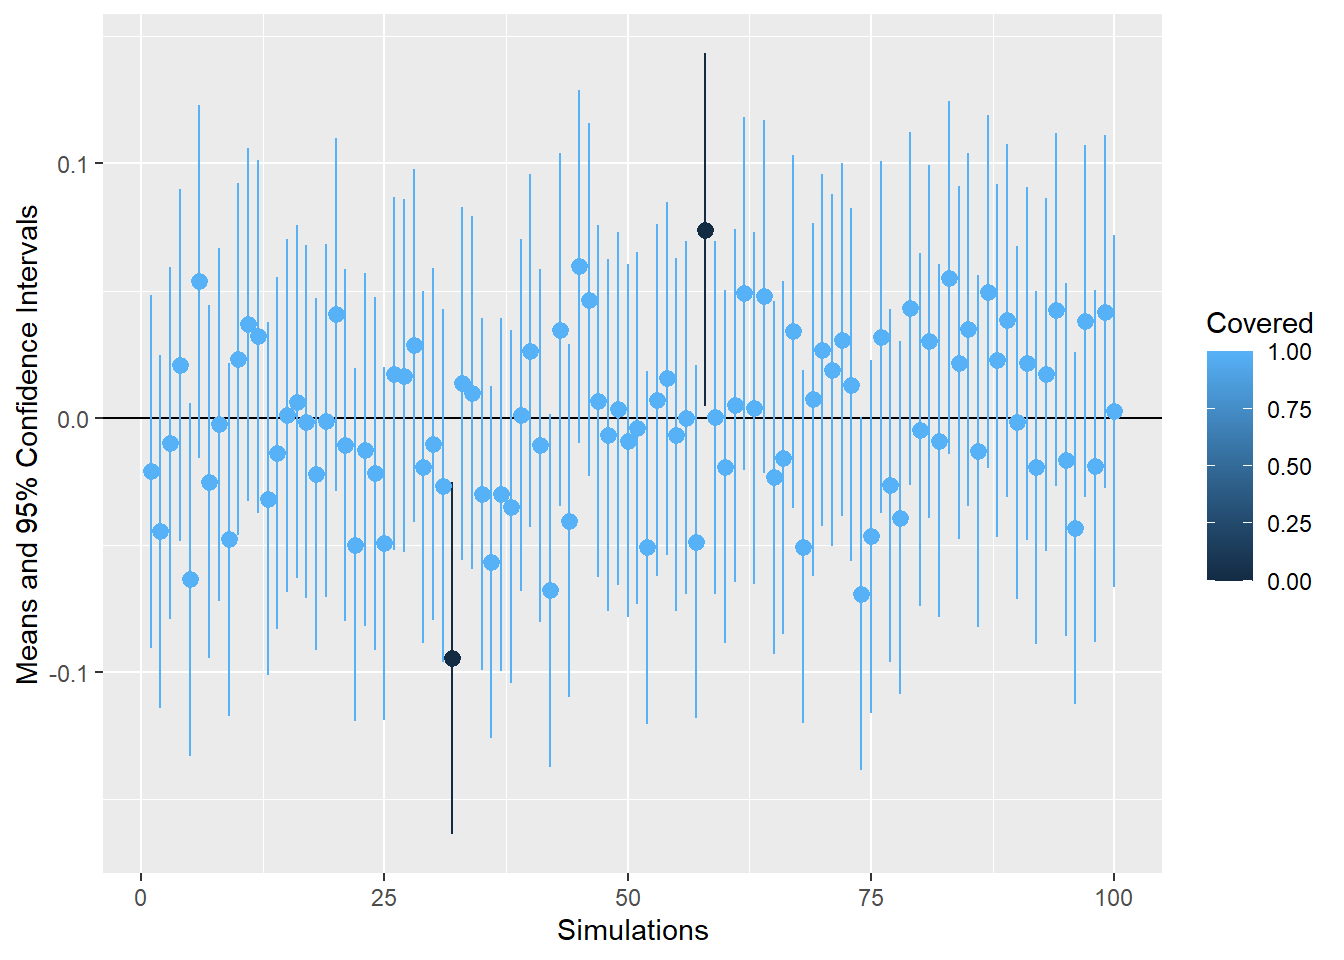
\includegraphics{Chapter_2_files/figure-latex/unnamed-chunk-7-1.pdf}
In this case only two out of 100 CI's do not include the true population mean.

\hypertarget{the-central-limit-theorem}{%
\section{The Central Limit Theorem}\label{the-central-limit-theorem}}

Here we will also try to illustrate the \href{https://en.wikipedia.org/wiki/Central_limit_theorem}{Central Limit Theorem}, in it's most basic form, with a very simple example.

First we draw 1000 samples (again of size 800), form , say, a \emph{Poisson} distribution, of course we could've drawn them from a uniform or an exponential as well.

Now we calculate the mean for each sample:

\begin{Shaded}
\begin{Highlighting}[]
\NormalTok{means }\OtherTok{\textless{}{-}}\NormalTok{ samples\_2 }\SpecialCharTok{\%\textgreater{}\%}
  \FunctionTok{lapply}\NormalTok{(., mean) }\SpecialCharTok{\%\textgreater{}\%}
  \FunctionTok{as.data.frame}\NormalTok{() }\SpecialCharTok{\%\textgreater{}\%}
  \FunctionTok{t}\NormalTok{()}
\end{Highlighting}
\end{Shaded}

And now we plot a histogram of the resulting means:

\begin{Shaded}
\begin{Highlighting}[]
\FunctionTok{hist}\NormalTok{(}\FunctionTok{t}\NormalTok{(means))}
\end{Highlighting}
\end{Shaded}

\begin{figure}
\centering
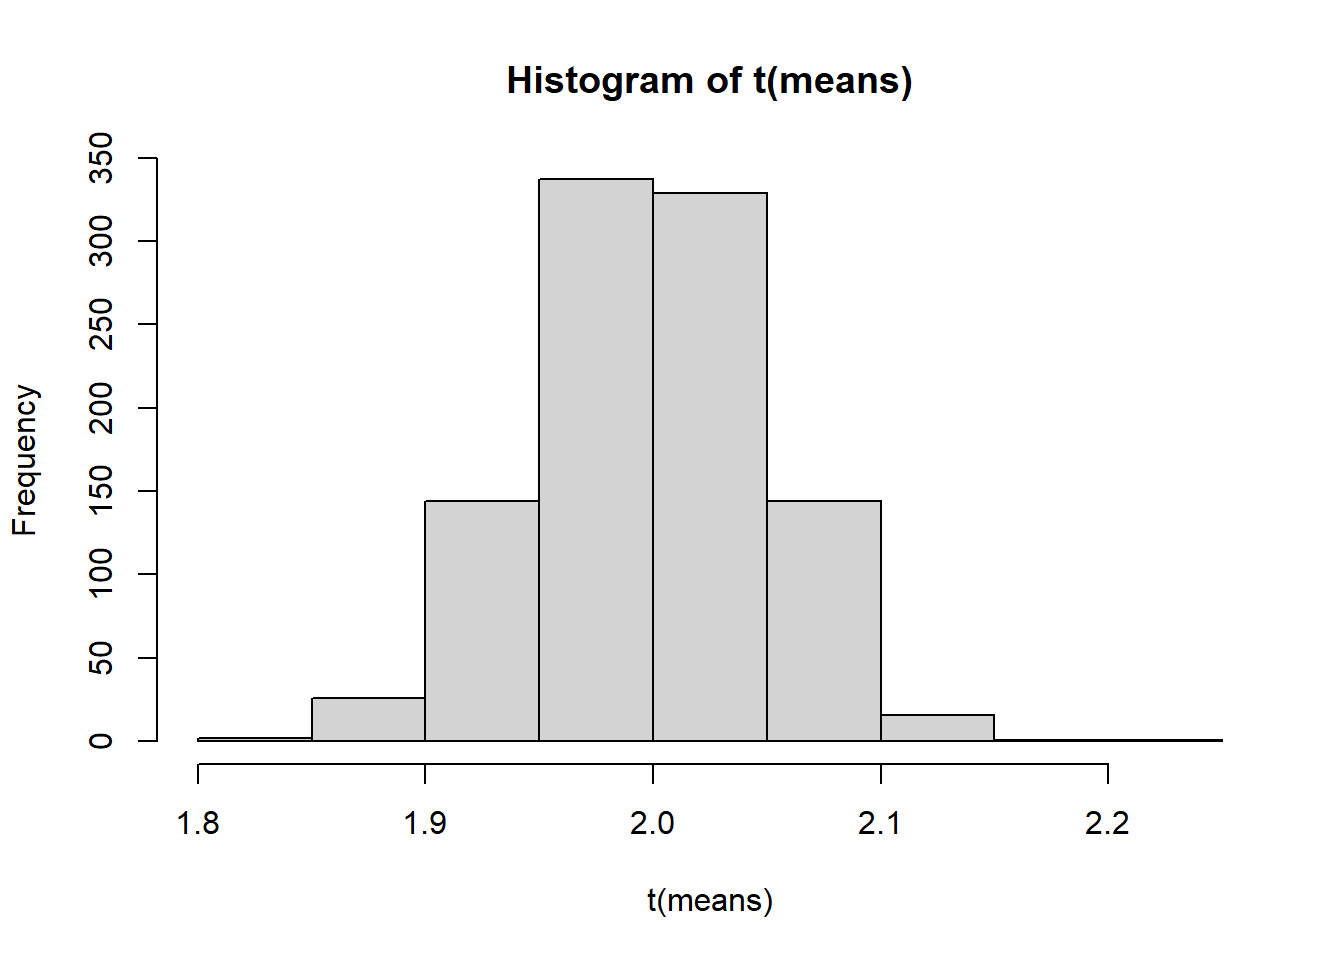
\includegraphics{Chapter_2_files/figure-latex/unnamed-chunk-10-1.pdf}
\caption{\label{fig:unnamed-chunk-10}Histogram of the sampling distribution of the mean}
\end{figure}

\hypertarget{informative-hypothesis-bayesian-testing-for-multi-level-models}{%
\chapter{Informative hypothesis (Bayesian) testing for multi-level models}\label{informative-hypothesis-bayesian-testing-for-multi-level-models}}

\hypertarget{example-for-citation}{%
\section{Example for citation}\label{example-for-citation}}

We will be using the \emph{Approximate Adjusted Fractional Bayes factor} proposed by \protect\hyperlink{ref-gu2018approximated}{Gu, Mulder, \& Hoijtink} (\protect\hyperlink{ref-gu2018approximated}{2018}), which is implemented in the R package \texttt{bain} (\protect\hyperlink{ref-bain}{Gu, Hoijtink, Mulder, \& van Lissa, 2021}).

We can reference like this \protect\hyperlink{ref-hoijtink2008bayesian}{Hoijtink, Klugkist, \& Boelen} (\protect\hyperlink{ref-hoijtink2008bayesian}{2008}) or like this (\protect\hyperlink{ref-hoijtink2008bayesian}{Hoijtink, Klugkist, \& Boelen, 2008})

\hypertarget{part-r-package-bain}{%
\chapter*{\texorpdfstring{(PART) \texttt{R} package \texttt{bain}}{(PART) R package bain}}\label{part-r-package-bain}}
\addcontentsline{toc}{chapter}{(PART) \texttt{R} package \texttt{bain}}

\hypertarget{introduction-to-bain}{%
\chapter{\texorpdfstring{Introduction to \texttt{bain}}{Introduction to bain}}\label{introduction-to-bain}}

\texttt{bain} is an acronym for \textbf{``Bayesian informative hypotheses evaluation''}.
It uses the \emph{Bayes factor} (\protect\hyperlink{ref-kass1995bayes}{Kass \& Raftery, 1995}) to evaluate hypotheses specified using \emph{equality} and \emph{inequality} constraints among (linear combinations of) parameters in a wide range of statistical models.

\hypertarget{available-tutorials}{%
\section{Available tutorials}\label{available-tutorials}}

Two tutorials are retrievable from the \texttt{bain} \href{https://informative-hypotheses.sites.uu.nl/software/bain/}{website} under the section \textbf{Tutorials}.

The first introducing Bayesian evaluation of informative hypotheses is provided by \protect\hyperlink{ref-hoijtink2019tutorial}{Hoijtink, Mulder, Lissa, \& Gu} (\protect\hyperlink{ref-hoijtink2019tutorial}{2019}). By reading the tutorial in combination with executing the analyses contained in \texttt{easyBFtutorial.R} and \texttt{BFtutorial.R} (available on the aforementioned website) you will quickly learn the basics of Bayesian hypothesis evaluation.

The second containing introduction to Bayesian evaluation of informative hypotheses in the context of structural equation models is provided by \protect\hyperlink{ref-van2021teacher}{Van Lissa et al.} (\protect\hyperlink{ref-van2021teacher}{2021})\footnote{Users are advised to read these tutorials and this vignette before using \texttt{bain}.}.

An overview of all other relevant papers concerning informative hypotheses testing and the package \texttt{bain} can be found \href{https://informative-hypotheses.sites.uu.nl/publications/}{here}.

\hypertarget{usage}{%
\section{Usage}\label{usage}}

This is how a general call to \texttt{bain} looks like:

\texttt{results\ \ \textless{}-\ bain(x,\ hypothesis,\ fraction\ =\ 1,\ ...)}

\hypertarget{arguments}{%
\subsection{Arguments}\label{arguments}}

\begin{itemize}
\tightlist
\item
  \texttt{x}
  An R object containing the outcome of a statistical analysis. Currently, the following objects can be processed:
\end{itemize}

\begin{enumerate}
\def\labelenumi{\arabic{enumi})}
\tightlist
\item
  \texttt{t\_test()} objects (Student's t-test, Welch's t-test, paired samples t-test, one-group t-test, equivalence test). Note that, \texttt{t\_test} can be used in the same way as \texttt{t.test}.
\item
  \texttt{lm()} objects (ANOVA, ANCOVA, multiple regression).
\item
  \texttt{lavaan} objects generated with the \texttt{sem()}, \texttt{cfa()}, and
  \texttt{growth} functions.
\item
  A named vector containing the estimates resulting from a statistical analysis. Using this option triggers the \texttt{bain.default()} method. Note that, named means that each estimate has to be named such that it can be referred to in hypotheses.
\item
  Wrapper functions for repeated measures ANOVA(\ldots) and linear two-level models built with \texttt{lmer} (TBA when finished).
\end{enumerate}

\begin{itemize}
\item
  \texttt{hypothesis} A character string containing the informative hypotheses to evaluate
  (see section 3.2.2).
\item
  \texttt{fraction\ =\ 1} A number representing the fraction of information in the data used to construct the prior distribution (see, for example, \protect\hyperlink{ref-gu2018approximated}{Gu, Mulder, \& Hoijtink} (\protect\hyperlink{ref-gu2018approximated}{2018})). The default value 1 denotes the minimal fraction, 2 denotes twice the minimal fraction, etc. The examples in chapter 5 show how the \texttt{fraction} can be employed to execute a sensitivity analysis. See also \protect\hyperlink{ref-hoijtink2019tutorial}{Hoijtink, Mulder, Lissa, \& Gu} (\protect\hyperlink{ref-hoijtink2019tutorial}{2019}) for more details.
\item
  \texttt{...} Additional arguments (see next chapter).
\end{itemize}

\hypertarget{the-specification-of-hypotheses}{%
\subsection{\texorpdfstring{The specification of \texttt{hypotheses}}{The specification of hypotheses}}\label{the-specification-of-hypotheses}}

\texttt{hypotheses} is a character string that specifies which (informative)
hypotheses have to be evaluated. A simple example is \texttt{hypotheses\ \textless{}-\ "a\ \textgreater{}\ b\ \textgreater{}\ c;\ a\ =\ b\ =\ c;"} which specifies two hypotheses using three estimates with
names ``a,'' ``b,'' and ``c,'' respectively.

The hypotheses specified have to adhere to the following rules (\texttt{bain} may still run if you
deviate from the rules, however, the output will be nonsense):

\begin{itemize}
\tightlist
\item
  When using \texttt{bain} with a \texttt{lm} or \texttt{t\_test} or \texttt{lavaan} object,
  (unique abbreviations of) the names
  displayed by \texttt{coef(x)} have to be used (but see the section \ref{lavaan} for additional instructions if multiple group
  analyses are executed and/or parameters are labeled). If,
  for example, the names are \texttt{cat} and \texttt{dog}, \texttt{c}
  and \texttt{d} would be unique abbreviations. If, for example, the names are \texttt{cato}
  and \texttt{cata} the whole
  names have to be used.
\item
  When using \texttt{bain} with a named vector, parameters are referred to using
  the names specified in \texttt{names()}.
\item
  Linear combinations of parameters must be specified adhering to the
  following rules:
\end{itemize}

\begin{enumerate}
\def\labelenumi{\alph{enumi})}
\item
  Each parameter name is used at most once.
\item
  Each parameter name may or may not be pre-multiplied with a number.
\item
  A constant may be added or subtracted from each parameter name.
\item
  A linear combination can also be a single number.

  Examples are: \texttt{3\ *\ a\ +\ 5}; \texttt{a\ +\ 2\ *\ b\ +\ 3\ *\ c\ -\ 2}; \texttt{a\ -\ b}; and \texttt{5}.
\end{enumerate}

\begin{itemize}
\tightlist
\item
  (Linear combinations of) parameters can be constrained using \textless, \textgreater, and
  =. For example, \texttt{a\ \textgreater{}\ 0} or
  \texttt{a\ \textgreater{}\ b\ =\ 0} or \texttt{2\ *\ a\ \textless{}\ b\ +\ c\ \textgreater{}\ 5}.
\item
  The ampersand \texttt{\&} can be used to combine different parts of a hypothesis.
  For example, \texttt{a\ \textgreater{}\ b\ \&\ b\ \textgreater{}\ c} which is equivalent to \texttt{a\ \textgreater{}\ b\ \textgreater{}\ c} or
  \texttt{a\ \textgreater{}\ 0\ \&\ b\ \textgreater{}\ 0\ \&\ c\ \textgreater{}\ 0}.
\item
  Sets of (linear combinations of) parameters subjected to the same
  constraints can be specified using (). For
  example, \texttt{a\ \textgreater{}\ (b,c)} which is equivalent to \texttt{a\ \textgreater{}\ b\ \&\ a\ \textgreater{}\ c}.
\item
  The specification of a hypothesis is completed by typing ; For example,
  \texttt{hypotheses\ \textless{}-\ "a\ \textgreater{}\ b\ \textgreater{}\ c;\ a\ =\ b\ =\ c;"}, specifies two hypotheses.
\item
  Hypotheses have to be compatible, non-redundant and possible. What
  these terms mean will be elaborated below.
\end{itemize}

\textbf{The set of hypotheses has to be compatible.} For the statistical
background of this requirement see \protect\hyperlink{ref-gu2018approximated}{Gu, Mulder, \& Hoijtink} (\protect\hyperlink{ref-gu2018approximated}{2018}). Usually the
sets of hypotheses specified by researchers are compatible, and if not,
\texttt{bain} will return an error message. The following steps can be used to
determine if a set of hypotheses is compatible:

\begin{enumerate}
\def\labelenumi{\arabic{enumi})}
\tightlist
\item
  Replace a range constraint, e.g., \texttt{1\ \textless{}\ a1\ \textless{}\ 3}, by an equality
  constraint in which the parameter involved is equated to the midpoint of the
  range, that is, \texttt{a1\ =\ 2}.
\item
  Replace in each hypothesis the \textless{} and \textgreater{} by =. For example,
  \texttt{a1\ =\ a2\textgreater{}\ a3\ \textgreater{}\ a4} becomes \texttt{a1\ =\ a2\ =\ a3\ =\ a4}.
\item
  The hypotheses are compatible if there is at least one solution to the
  resulting set of equations. For the two hypotheses considered under 1. and
  2., the solution is \texttt{a1\ =\ a2\ =\ a3\ =\ a4\ =\ 2}. An example of two non-compatible
  hypotheses is \texttt{hypotheses\ \textless{}-\ "a\ =\ 0;\ a\ \textgreater{}\ 2;"} because there is no
  solution to the equations \texttt{a=0} and \texttt{a=2}.
\end{enumerate}

\textbf{Each hypothesis in a set of hypotheses has to be non-redundant.} A
hypothesis is redundant if it can also be specified with fewer constraints.
For example, \texttt{a\ =\ b\ \&\ a\ \textgreater{}\ 0\ \&\ b\ \textgreater{}\ 0} is redundant because it can also be
specified as \texttt{a\ =\ b\ \&\ a\ \textgreater{}\ 0}. \texttt{bain} will work correctly if
hypotheses specified using only \textless{} and \textgreater{} are redundant. \texttt{bain} will
return an error message if hypotheses specified using at least one = are
redundant.

\textbf{Each hypothesis in a set of hypotheses has to be possible.} An
hypothesis is impossible if estimates in agreement with the hypothesis do not
exist. For example: values for \texttt{a,\ b,\ c} in agreement with \texttt{a\ \textgreater{}\ b\ \textgreater{}\ c\ \&\ a\ \textless{}\ c} do not exist. It is the responsibility of the user to ensure that the
hypotheses specified are possible. If not, \texttt{bain} will either return an
error message or render an output table containing \texttt{Inf}'s.

\hypertarget{output}{%
\subsection{Output}\label{output}}

The commands \texttt{bain()} or \texttt{results\textless{}-bain()} followed by
\texttt{results} or \texttt{print(results)} will render the default (most
important) output from \texttt{bain}. These concern for each hypothesis
specified in \texttt{hypotheses} the fit, complexity, Bayes factor versus
the unconstrained hypothesis, Bayes factor versus its
complement, posterior model probability (based on equal prior model
probabilities) excluding the unconstrained hypothesis, posterior model
probability including the unconstrained hypothesis, and posterior model
probability of each hypothesis specified and their joint complement.
Note that, all the posterior model probabilities are computed from
the Bayes factors of each hypothesis versus the unconstrained hypothesis.
In \protect\hyperlink{ref-hoijtink2019tutorial}{Hoijtink, Mulder, Lissa, \& Gu} (\protect\hyperlink{ref-hoijtink2019tutorial}{2019}) it is elaborated how these quantities
(and the other
output presented below) should be interpreted. Additionally, using
\texttt{summary(results,\ ci=0.95)}, a descriptives matrix can be obtained
in which for each estimate, the name, the value, and a 95\% central
credibility interval is presented.

The following commands can be used to
retrieve the default and additional information from the \texttt{bain} output
object:

\begin{itemize}
\tightlist
\item
  \texttt{results\$fit} renders the default output, \texttt{results\$fit\$Fit}
  contains only the column containing the fit of each hypothesis. In the last
  command \texttt{Fit} can be replaced by \texttt{Com}, \texttt{BF}, \texttt{BF.u}, \texttt{BF.c}, \texttt{PMPa},
  \texttt{PMPb}, \texttt{PMPc} to obtain the information in the corresponding columns of the
  default output. Note that, in the columns \texttt{BF} and \texttt{BF.c} the Bayes factor of the
  hypothesis at hand versus its complement is displayed. In the column \texttt{BF.u} the
  Bayes factor of the hypothesis at hand versus the unconstrained hypothesis is
  displayed. \texttt{PMPa} renders the posterior model probabilities (based on equal
  prior model probabilities) of the hypotheses specified. \texttt{PMPb} renders
  the posterior model probabilities (based on equal
  prior model probabilities) of the hypotheses specified plus the unconstrained
  hypothesis. \texttt{PMPc} renders the posterior model probabilities (based on equal
  prior model probabilities) of the hypotheses specified plus the complement of
  the union of these hypotheses. If, in the latter case, the complexity of the
  complement of the union of all hypotheses specified is smaller than .05, the
  hypotheses specified (almost) completely cover the parameter space. In this
  case \texttt{PMPc} is not provided and instead \texttt{PMPa} should be used.
\item
  \texttt{results\$BFmatrix} contains the matrix containing the mutual Bayes
  factors of the hypotheses specified in \texttt{hypotheses}.
\item
  \texttt{results\$b} contains for each of the groups in the analysis the
  fraction of information of the data in the group at hand used to specify the
  covariance matrix of the prior distribution.
\item
  \texttt{results\$prior} contains the covariance matrix of the prior
  distribution.
\item
  \texttt{results\$posterior} contains the covariance matrix of the
  posterior distribution.
\item
  \texttt{results\$call} displays the call to \texttt{bain}.
\item
  \texttt{results\$model} displays the named vector or the R object that is input to \texttt{bain}.
\item
  \texttt{results\$n} displays the sample sizes per group.
\item
  \texttt{results\$independent\_restrictions} displays the number of
  independent constraints in the set of hypotheses under consideration. Note that,
  in \protect\hyperlink{ref-gu2018approximated}{Gu, Mulder, \& Hoijtink} (\protect\hyperlink{ref-gu2018approximated}{2018}) and \protect\hyperlink{ref-hoijtink2019bayesian}{Hoijtink, Gu, \& Mulder} (\protect\hyperlink{ref-hoijtink2019bayesian}{2019}) the
  definition given was misprinted (besides R and S also r and s should have been
  added to the definition).
\item
  \texttt{results\$fit\$Fit\_eq} displays the fit of the equality constrained
  part of each hypothesis. Replacing \texttt{Fit\_eq} by \texttt{Fit\_in}, renders
  the fit of the inequality constrained part of an hypothesis conditional on
  the fit of the equality constrained part. \texttt{Com\_eq}, and \texttt{Com\_in},
  respectively, are the complexity counterparts of \texttt{Fit\_eq}, and
  \texttt{Fit\_in}.
\end{itemize}

Note that, if you have specified two hypotheses that both have a small
\texttt{BF.u} (close to zero), then there is no support in the data for these
hypotheses. In these cases the corresponding entry in \texttt{results\$BFmatrix}
(the Bayes factor comparing both hypotheses) is very unstable and should
only be interpreted if repeated analyses using different seeds
(see \texttt{set.seed()}) render about the same results.

\hypertarget{example-output}{%
\subsubsection{Example output}\label{example-output}}

The following example is aimed at illustrating the output from \texttt{bain}. The specifics on how to actually use \texttt{bain} for testing hypotheses about the parameters of different statistical models are given in the next chapter.

In this example we will use \texttt{bain} to test the following two (informative) hypotheses concerning the parameters of a multiple linear regression model, with three (continuous) predictors:

\begin{itemize}
\tightlist
\item
  \(H_1: \beta_1 > 0;\; \beta_2 > 0;\; \beta_3 >0\)
\item
  \(H_2: \beta_1 = \beta_2 < \beta_3\)
\end{itemize}

\begin{enumerate}
\def\labelenumi{(\arabic{enumi})}
\tightlist
\item
  The default output:
\end{enumerate}

\begin{Shaded}
\begin{Highlighting}[]
\FunctionTok{print}\NormalTok{(results)}
\end{Highlighting}
\end{Shaded}

\begin{verbatim}
## Bayesian informative hypothesis testing for an object of class lm (continuous predictors):
## 
##    Fit   Com   BF.u   BF.c    PMPa  PMPb 
## H1 0.871 0.032 27.295 204.167 0.747 0.727
## H2 2.637 0.285 9.247  9.247   0.253 0.246
## Hu                                  0.027
## 
## Hypotheses:
##   H1: age>0&peabody>0&prenumb>0
##   H2: age=peabody<prenumb
## 
## Note: BF.u denotes the Bayes factor of the hypothesis at hand versus the unconstrained hypothesis Hu. BF.c denotes the Bayes factor of the hypothesis at hand versus its complement.
\end{verbatim}

The output consists of several parts:

\begin{enumerate}
\def\labelenumi{(\alph{enumi})}
\tightlist
\item
  On the top, it is stated from which type of \texttt{R} object the parameter estimates come from;
\item
  The most important part of the output are the results from \texttt{bain} presented in the middle. Here, for each hypothesis, the fit, complexity, the BF of the hypothesis against the unconstrained, the BF of the hypothesis against it's compliment, and the posterior model probabilities are printed in each row. For example, for \(H_1 =\beta_1 > 0;\; \beta_2 > 0;\; \beta_3 >0\), the fit and complexity are equal to 0.871 and 0.032, respectively, resulting in a \(BF_{1u}\) = 27.3. The value for \(BF_{1u}\) suggests that \(H_1\) is 27 times as likely compared to \(H_u\). The value for \texttt{PMPa} suggests that the posterior probability of \(H_1\) \emph{given} the data is around 0.75, assuming equal prior probabilities. The value for \texttt{PMPb} suggests that the posterior probability of \(H_1 + H_u\) \emph{given} the data is around 0.73, assuming equal prior probabilities. If we would like to obtain the BF for \(H_1\) against \(H_2\) (\(BF_{12}\)), then we just need to take the ratio of the two BF's against the unconstrained hypothesis. In this case, \[BF_{12} = \frac{27.3}{9.2} \approx 3\]
\end{enumerate}

which means that the support in the data is 3 times larger for \(H_1\) compared to \(H_2\);

\begin{enumerate}
\def\labelenumi{(\alph{enumi})}
\setcounter{enumi}{2}
\tightlist
\item
  The tested hypotheses are printed in the output, just below the results;
\item
  The output ends with a note explaining the difference between the two types BF's printed in the main part of the results (b).
\end{enumerate}

\begin{enumerate}
\def\labelenumi{(\arabic{enumi})}
\setcounter{enumi}{1}
\tightlist
\item
  Descriptive matrix:
\end{enumerate}

\begin{Shaded}
\begin{Highlighting}[]
\FunctionTok{summary}\NormalTok{(results)}
\end{Highlighting}
\end{Shaded}

\begin{verbatim}
##   Parameter   n   Estimate          lb        ub
## 1       age 240 0.05797594 -0.04043979 0.1563917
## 2   peabody 240 0.14781779  0.03457188 0.2610637
## 3   prenumb 240 0.56740695  0.46067277 0.6741411
\end{verbatim}

\begin{enumerate}
\def\labelenumi{(\arabic{enumi})}
\setcounter{enumi}{2}
\tightlist
\item
  Obtaining the separate values contained within the \texttt{results} object. Here we only present how to obtain the value for the fit, of course, as mentioned above different values contained within the \texttt{results} object can be obtained by changing what comes after the \texttt{\$} in the code below:
\end{enumerate}

\begin{Shaded}
\begin{Highlighting}[]
\NormalTok{results}\SpecialCharTok{$}\NormalTok{fit}
\end{Highlighting}
\end{Shaded}

\begin{verbatim}
##      Fit_eq    Com_eq    Fit_in     Com_in       Fit        Com         BF
## H1 1.000000 1.0000000 0.8705764 0.03189549 0.8705764 0.03189549 204.167441
## H2 2.636926 0.5703344 1.0000000 0.50000000 2.6369262 0.28516720   9.246948
## Hu       NA        NA        NA         NA        NA         NA         NA
##         PMPa       PMPb      BF.u       BF.c
## H1 0.7469474 0.72705089 27.294657 204.167441
## H2 0.2530526 0.24631200  9.246948   9.246948
## Hu        NA 0.02663711        NA         NA
\end{verbatim}

\hypertarget{hands-on-examples-using-bain}{%
\chapter{\texorpdfstring{Hands-on examples using \texttt{bain}}{Hands-on examples using bain}}\label{hands-on-examples-using-bain}}

Unless indicated otherwise, the examples that follow below use a simulated
data set inspired by the \texttt{Sesame\ Street} data set presented in:
\protect\hyperlink{ref-stevens1996applied}{Stevens} (\protect\hyperlink{ref-stevens1996applied}{1996}). This data set is included in the
\texttt{bain} package.

The variables contained in \texttt{sesamesim} are subsequently:

\begin{itemize}
\tightlist
\item
  \texttt{sex} (1 = boy, 2 = girl) of the child
\item
  \texttt{site} (1 = disadvantaged inner city, 2 = advantaged suburban , 3 =
  advantaged rural,
  4 = disadvantaged rural, 5 = disadvantaged Spanish speaking) from which
  the child originates
\item
  \texttt{settin}g (1 = at home, 2 = at school) in which the child watches sesame
  street
\item
  \texttt{age} (in months) of the child
\item
  \texttt{viewenc} (0 = no, 1 = yes), whether or not the child is encouraged to
  watch Sesame Street
\item
  \texttt{peabody} (mental age) score of the child (higher score is higher mental
  age)
\item
  \texttt{prenumb} (score on a numbers test before watching Sesame Street for a
  year)
\item
  \texttt{postnumb} (score on a numbers test after watching Sesame Street for a
  year)
\item
  \texttt{funumb} (follow up numbers test score measured one year after postnumb)
\item
  \texttt{Bb} Knowledge of body parts before
\item
  \texttt{Bl} Knowledge of letters before
\item
  \texttt{Bf} Knowledge of forms before
\item
  \texttt{Bn} Knowledge of numbers before
\item
  \texttt{Br} Knowledge of relations before
\item
  \texttt{Bc} Knowledge of classifications before
\item
  \texttt{Ab} Knowledge of body parts after
\item
  \texttt{Al} Knowledge of letters after
\item
  \texttt{Af} Knowledge of forms after
\item
  \texttt{An} Knowledge of numbers after
\item
  \texttt{Ar} Knowledge of relations after
\item
  \texttt{Ac} Knowledge of classifications after
\end{itemize}

The examples that follow below are organized in four categories:

\begin{enumerate}
\def\labelenumi{\arabic{enumi})}
\tightlist
\item
  running \texttt{bain} with a \texttt{t\_test} object
\item
  running \texttt{bain} with a \texttt{lm} object
\item
  running \texttt{bain} with a \texttt{lavaan} object
\item
  running bain with a named vector
\end{enumerate}

Load the \texttt{bain} package which includes the simulated \texttt{sesamesim} data set:

\begin{Shaded}
\begin{Highlighting}[]
\FunctionTok{library}\NormalTok{(bain)}
\end{Highlighting}
\end{Shaded}

\hypertarget{using-bain-with-a-t_test-object}{%
\section{\texorpdfstring{Using \texttt{bain} with a \texttt{t\_test} object}{Using bain with a t\_test object}}\label{using-bain-with-a-t_test-object}}

If a \texttt{t\_test} object is used, the main output table is
labeled: \emph{``Bayesian informative hypothesis testing for an objectof class t\_test''} (which denotes that a \texttt{t-test} was executed).

\textbf{Options:}

\begin{enumerate}
\def\labelenumi{\alph{enumi})}
\tightlist
\item
  Bayesian Student's t-test (equal within group variances)
\item
  Bayesian Welch's t-test (unequal within group variances
\item
  Bayesian paired samples t-test
\item
  Bayesian one group t-test
\item
  Bayesian Equivalence test
\end{enumerate}

\textbf{Main steps:}

\begin{enumerate}
\def\labelenumi{\arabic{enumi})}
\item
  Execute the analysis with \texttt{t\_test()}. Note that, \texttt{t\_test} will apply list-wise deletion if there are cases with missing values in the variables used.
\item
  Call `bain:
\end{enumerate}

\begin{itemize}
\item
  \texttt{set.seed(seed)}. Set \texttt{seed} equal to an integer number to create a repeatable random number sequence. \texttt{bain} uses sampling to compute Bayes factors and posterior model probabilities. It is therefore recommended to run analyses with two different seeds to ensure stability of the results.
\item
  When \texttt{t\_test()} is used, hypotheses have to be specified using the names \texttt{x}, \texttt{y}, or \texttt{difference}.
\end{itemize}

\begin{enumerate}
\def\labelenumi{\arabic{enumi})}
\setcounter{enumi}{2}
\item
  \texttt{results\ \textless{}-\ bain(x,hypotheses,fraction\ =\ 1)}
  \texttt{fraction\ =\ 1}represents the fraction of information in the data used to construct the prior distribution (see, for example, \protect\hyperlink{ref-gu2018approximated}{Gu, Mulder, \& Hoijtink} (\protect\hyperlink{ref-gu2018approximated}{2018})). The default value 1 denotes the minimal fraction, 2 denotes twice the minimal fraction, etc.
\item
  \texttt{print(results)} Print the results of an analysis with
  \texttt{bain}.
\item
  \texttt{summary(results,\ ci=0.95)} Present estimates and credibility intervals for the parameters used to specify the \texttt{hypotheses}. \texttt{ci} can be used to specify the confidence level of the credibility intervals.
\end{enumerate}

\hypertarget{students-t-test-equal-within-group-variances}{%
\subsection{Student's t-test (equal within group variances):}\label{students-t-test-equal-within-group-variances}}

\begin{enumerate}
\def\labelenumi{\arabic{enumi})}
\tightlist
\item
  Execute the analysis with \texttt{t\_test()}:
\end{enumerate}

\begin{Shaded}
\begin{Highlighting}[]
\CommentTok{\# collect the data for the boys in the vector x and for the girls in the}
\CommentTok{\# vector y}
\NormalTok{x}\OtherTok{\textless{}{-}}\NormalTok{sesamesim}\SpecialCharTok{$}\NormalTok{postnumb[}\FunctionTok{which}\NormalTok{(sesamesim}\SpecialCharTok{$}\NormalTok{sex}\SpecialCharTok{==}\DecValTok{1}\NormalTok{)]}
\NormalTok{y}\OtherTok{\textless{}{-}}\NormalTok{sesamesim}\SpecialCharTok{$}\NormalTok{postnumb[}\FunctionTok{which}\NormalTok{(sesamesim}\SpecialCharTok{$}\NormalTok{sex}\SpecialCharTok{==}\DecValTok{2}\NormalTok{)]}
\CommentTok{\# execute student\textquotesingle{}s t{-}test (with assumed equal variances)}
\NormalTok{ttest }\OtherTok{\textless{}{-}} \FunctionTok{t\_test}\NormalTok{(x,y,}\AttributeTok{paired =} \ConstantTok{FALSE}\NormalTok{, }\AttributeTok{var.equal =} \ConstantTok{TRUE}\NormalTok{)}
\end{Highlighting}
\end{Shaded}

\begin{enumerate}
\def\labelenumi{\arabic{enumi})}
\setcounter{enumi}{1}
\tightlist
\item
  Call \texttt{bain} \& 3) Store the output in a \texttt{results} object:
\end{enumerate}

\begin{Shaded}
\begin{Highlighting}[]
\CommentTok{\# set a seed value}
\FunctionTok{set.seed}\NormalTok{(}\DecValTok{100}\NormalTok{)}
\CommentTok{\# test hypotheses with bain. The names of the means are x and y.}
\NormalTok{results }\OtherTok{\textless{}{-}} \FunctionTok{bain}\NormalTok{(ttest, }\StringTok{"x = y; x \textgreater{} y; x \textless{} y"}\NormalTok{, }\AttributeTok{fraction =} \DecValTok{1}\NormalTok{)}
\end{Highlighting}
\end{Shaded}

\begin{enumerate}
\def\labelenumi{\arabic{enumi})}
\setcounter{enumi}{2}
\tightlist
\item
  Print the results:
\end{enumerate}

\begin{Shaded}
\begin{Highlighting}[]
\FunctionTok{print}\NormalTok{(results)}
\end{Highlighting}
\end{Shaded}

\begin{verbatim}
## Bayesian informative hypothesis testing for an object of class t_test:
## 
##    Fit   Com   BF.u   BF.c   PMPa  PMPb 
## H1 0.183 0.016 11.583 11.583 0.853 0.794
## H2 0.777 0.500 1.554  3.481  0.114 0.107
## H3 0.223 0.500 0.446  0.287  0.033 0.031
## Hu                                 0.069
## 
## Hypotheses:
##   H1: x=y
##   H2: x>y
##   H3: x<y
## 
## Note: BF.u denotes the Bayes factor of the hypothesis at hand versus the unconstrained hypothesis Hu. BF.c denotes the Bayes factor of the hypothesis at hand versus its complement.
\end{verbatim}

\begin{enumerate}
\def\labelenumi{\arabic{enumi})}
\setcounter{enumi}{3}
\tightlist
\item
  Summary: estimates and credibility intervals:
\end{enumerate}

\begin{Shaded}
\begin{Highlighting}[]
\FunctionTok{summary}\NormalTok{(results)}
\end{Highlighting}
\end{Shaded}

\begin{verbatim}
##   Parameter   n Estimate       lb       ub
## 1         x 115 30.09565 27.79295 32.39836
## 2         y 125 28.85600 26.64732 31.06468
\end{verbatim}

\hypertarget{welchs-t-test-unequal-within-group-variances}{%
\subsection{Welch's t-test (unequal within group variances):}\label{welchs-t-test-unequal-within-group-variances}}

\begin{enumerate}
\def\labelenumi{\arabic{enumi})}
\tightlist
\item
  Execute the analysis with \texttt{t\_test()}:
\end{enumerate}

\begin{Shaded}
\begin{Highlighting}[]
\NormalTok{wtest }\OtherTok{\textless{}{-}} \FunctionTok{t\_test}\NormalTok{(x,y,}\AttributeTok{paired =} \ConstantTok{FALSE}\NormalTok{, }\AttributeTok{var.equal =} \ConstantTok{FALSE}\NormalTok{) }
\end{Highlighting}
\end{Shaded}

\begin{enumerate}
\def\labelenumi{\arabic{enumi})}
\setcounter{enumi}{1}
\tightlist
\item
  Call \texttt{bain} \& 3) Store the output in a \texttt{results} object:
\end{enumerate}

\begin{Shaded}
\begin{Highlighting}[]
\FunctionTok{set.seed}\NormalTok{(}\DecValTok{100}\NormalTok{)}
\NormalTok{results }\OtherTok{\textless{}{-}} \FunctionTok{bain}\NormalTok{(wtest, }\StringTok{"x = y; x \textgreater{} y; x \textless{} y"}\NormalTok{)}
\end{Highlighting}
\end{Shaded}

\begin{enumerate}
\def\labelenumi{\arabic{enumi})}
\setcounter{enumi}{2}
\tightlist
\item
  Print the results:
\end{enumerate}

\begin{Shaded}
\begin{Highlighting}[]
\FunctionTok{print}\NormalTok{(results)}
\end{Highlighting}
\end{Shaded}

\begin{verbatim}
## Bayesian informative hypothesis testing for an object of class t_test:
## 
##    Fit   Com   BF.u   BF.c   PMPa  PMPb 
## H1 0.183 0.016 11.586 11.586 0.853 0.794
## H2 0.776 0.500 1.552  3.467  0.114 0.106
## H3 0.224 0.500 0.448  0.288  0.033 0.031
## Hu                                 0.069
## 
## Hypotheses:
##   H1: x=y
##   H2: x>y
##   H3: x<y
## 
## Note: BF.u denotes the Bayes factor of the hypothesis at hand versus the unconstrained hypothesis Hu. BF.c denotes the Bayes factor of the hypothesis at hand versus its complement.
\end{verbatim}

\begin{enumerate}
\def\labelenumi{\arabic{enumi})}
\setcounter{enumi}{3}
\tightlist
\item
  Summary: estimates and credibility intervals:
\end{enumerate}

\begin{Shaded}
\begin{Highlighting}[]
\FunctionTok{summary}\NormalTok{(results)}
\end{Highlighting}
\end{Shaded}

\begin{verbatim}
##   Parameter   n Estimate       lb       ub
## 1         x 115 30.09565 27.70909 32.48221
## 2         y 125 28.85600 26.72394 30.98806
\end{verbatim}

\hypertarget{paired-samples-t-test}{%
\subsection{Paired samples t-test:}\label{paired-samples-t-test}}

\begin{enumerate}
\def\labelenumi{\arabic{enumi})}
\tightlist
\item
  Execute the analysis with \texttt{t\_test()}:
\end{enumerate}

\begin{Shaded}
\begin{Highlighting}[]
\NormalTok{pttest }\OtherTok{\textless{}{-}} \FunctionTok{t\_test}\NormalTok{(sesamesim}\SpecialCharTok{$}\NormalTok{prenumb,sesamesim}\SpecialCharTok{$}\NormalTok{postnumb,}\AttributeTok{paired =} \ConstantTok{TRUE}\NormalTok{) }
\end{Highlighting}
\end{Shaded}

\begin{enumerate}
\def\labelenumi{\arabic{enumi})}
\setcounter{enumi}{1}
\tightlist
\item
  Call \texttt{bain} \& 3) Store the output in a \texttt{results} object:
\end{enumerate}

\begin{Shaded}
\begin{Highlighting}[]
\CommentTok{\# set a seed value}
\FunctionTok{set.seed}\NormalTok{(}\DecValTok{100}\NormalTok{)}
\CommentTok{\# test hypotheses with bain. The names of the means are x and y.}
\NormalTok{results }\OtherTok{\textless{}{-}} \FunctionTok{bain}\NormalTok{(pttest, }\StringTok{"difference=0; difference\textgreater{}0; difference\textless{}0"}\NormalTok{)}
\end{Highlighting}
\end{Shaded}

\begin{enumerate}
\def\labelenumi{\arabic{enumi})}
\setcounter{enumi}{2}
\tightlist
\item
  Print the results:
\end{enumerate}

\begin{Shaded}
\begin{Highlighting}[]
\FunctionTok{print}\NormalTok{(results)}
\end{Highlighting}
\end{Shaded}

\begin{verbatim}
## Bayesian informative hypothesis testing for an object of class t_test:
## 
##    Fit   Com   BF.u  BF.c               PMPa  PMPb 
## H1 0.000 0.042 0.000 0.000              0.000 0.000
## H2 0.000 0.500 0.000 0.000              0.000 0.000
## H3 1.000 0.500 2.000 22919082073133.293 1.000 0.667
## Hu                                            0.333
## 
## Hypotheses:
##   H1: difference=0
##   H2: difference>0
##   H3: difference<0
## 
## Note: BF.u denotes the Bayes factor of the hypothesis at hand versus the unconstrained hypothesis Hu. BF.c denotes the Bayes factor of the hypothesis at hand versus its complement.
\end{verbatim}

\begin{enumerate}
\def\labelenumi{\arabic{enumi})}
\setcounter{enumi}{3}
\tightlist
\item
  Summary: estimates and credibility intervals:
\end{enumerate}

\begin{Shaded}
\begin{Highlighting}[]
\FunctionTok{summary}\NormalTok{(results)}
\end{Highlighting}
\end{Shaded}

\begin{verbatim}
##    Parameter   n  Estimate        lb        ub
## 1 difference 240 -8.691667 -9.895994 -7.487339
\end{verbatim}

\hypertarget{one-group-t-test}{%
\subsection{One group t-test}\label{one-group-t-test}}

\begin{enumerate}
\def\labelenumi{\arabic{enumi})}
\tightlist
\item
  Execute the analysis with \texttt{t\_test()}:
\end{enumerate}

\begin{Shaded}
\begin{Highlighting}[]
\CommentTok{\# compare post measurements with the reference value 30}
\NormalTok{ttest\_one\_gr }\OtherTok{\textless{}{-}} \FunctionTok{t\_test}\NormalTok{(sesamesim}\SpecialCharTok{$}\NormalTok{postnumb)}
\end{Highlighting}
\end{Shaded}

\begin{enumerate}
\def\labelenumi{\arabic{enumi})}
\setcounter{enumi}{1}
\tightlist
\item
  Call \texttt{bain} \& 3) Store the output in a \texttt{results} object:
\end{enumerate}

\begin{Shaded}
\begin{Highlighting}[]
\CommentTok{\# set a seed value}
\FunctionTok{set.seed}\NormalTok{(}\DecValTok{100}\NormalTok{)}
\CommentTok{\# test hypotheses with bain versus the reference value 30. Use x to refer to the mean}
\NormalTok{results }\OtherTok{\textless{}{-}} \FunctionTok{bain}\NormalTok{(ttest\_one\_gr, }\StringTok{"x=30; x\textgreater{}30; x\textless{}30"}\NormalTok{, }\AttributeTok{fraction =} \DecValTok{2}\NormalTok{)}
\end{Highlighting}
\end{Shaded}

\begin{enumerate}
\def\labelenumi{\arabic{enumi})}
\setcounter{enumi}{2}
\tightlist
\item
  Print the results:
\end{enumerate}

\begin{Shaded}
\begin{Highlighting}[]
\FunctionTok{print}\NormalTok{(results)}
\end{Highlighting}
\end{Shaded}

\begin{verbatim}
## Bayesian informative hypothesis testing for an object of class t_test:
## 
##    Fit   Com   BF.u  BF.c  PMPa  PMPb 
## H1 0.390 0.045 8.712 8.712 0.813 0.744
## H2 0.249 0.500 0.498 0.332 0.047 0.043
## H3 0.751 0.500 1.502 3.012 0.140 0.128
## Hu                               0.085
## 
## Hypotheses:
##   H1: x=30
##   H2: x>30
##   H3: x<30
## 
## Note: BF.u denotes the Bayes factor of the hypothesis at hand versus the unconstrained hypothesis Hu. BF.c denotes the Bayes factor of the hypothesis at hand versus its complement.
\end{verbatim}

\begin{enumerate}
\def\labelenumi{\arabic{enumi})}
\setcounter{enumi}{3}
\tightlist
\item
  Summary: estimates and credibility intervals:
\end{enumerate}

\begin{Shaded}
\begin{Highlighting}[]
\FunctionTok{summary}\NormalTok{(results)}
\end{Highlighting}
\end{Shaded}

\begin{verbatim}
##   Parameter   n Estimate       lb       ub
## 1         x 240    29.45 27.85743 31.04257
\end{verbatim}

\hypertarget{equivalence-test}{%
\subsection{Equivalence test}\label{equivalence-test}}

\begin{enumerate}
\def\labelenumi{\arabic{enumi})}
\tightlist
\item
  Execute the analysis with \texttt{t\_test()}:
\end{enumerate}

\begin{Shaded}
\begin{Highlighting}[]
\CommentTok{\# collect the data for the boys in the vector x and for the girs in the}
\CommentTok{\# vector y}
\NormalTok{x}\OtherTok{\textless{}{-}}\NormalTok{sesamesim}\SpecialCharTok{$}\NormalTok{postnumb[}\FunctionTok{which}\NormalTok{(sesamesim}\SpecialCharTok{$}\NormalTok{sex}\SpecialCharTok{==}\DecValTok{1}\NormalTok{)]}
\NormalTok{y}\OtherTok{\textless{}{-}}\NormalTok{sesamesim}\SpecialCharTok{$}\NormalTok{postnumb[}\FunctionTok{which}\NormalTok{(sesamesim}\SpecialCharTok{$}\NormalTok{sex}\SpecialCharTok{==}\DecValTok{2}\NormalTok{)]}
\CommentTok{\# execute student\textquotesingle{}s t{-}test}
\NormalTok{ttest\_eq }\OtherTok{\textless{}{-}} \FunctionTok{t\_test}\NormalTok{(x,y,}\AttributeTok{paired =} \ConstantTok{FALSE}\NormalTok{, }\AttributeTok{var.equal =} \ConstantTok{TRUE}\NormalTok{)}
\end{Highlighting}
\end{Shaded}

Compute the pooled within standard deviation using the variance of x:

\begin{Shaded}
\begin{Highlighting}[]
\CommentTok{\# (ttest$v[1]) and y (ttest$v[2])}
\NormalTok{pwsd }\OtherTok{\textless{}{-}} \FunctionTok{sqrt}\NormalTok{(((}\FunctionTok{length}\NormalTok{(x) }\SpecialCharTok{{-}}\DecValTok{1}\NormalTok{) }\SpecialCharTok{*}\NormalTok{ ttest}\SpecialCharTok{$}\NormalTok{v[}\DecValTok{1}\NormalTok{] }\SpecialCharTok{+}\NormalTok{ (}\FunctionTok{length}\NormalTok{(y)}\SpecialCharTok{{-}}\DecValTok{1}\NormalTok{) }\SpecialCharTok{*}\NormalTok{ ttest}\SpecialCharTok{$}\NormalTok{v[}\DecValTok{2}\NormalTok{])}\SpecialCharTok{/}
\NormalTok{((}\FunctionTok{length}\NormalTok{(x) }\SpecialCharTok{{-}}\DecValTok{1}\NormalTok{) }\SpecialCharTok{+}\NormalTok{ (}\FunctionTok{length}\NormalTok{(y) }\SpecialCharTok{{-}}\DecValTok{1}\NormalTok{)))}
\CommentTok{\# print pwsd in order to be able to include it in the hypothesis. Its value}
\FunctionTok{print}\NormalTok{(pwsd)}
\end{Highlighting}
\end{Shaded}

\begin{verbatim}
## [1] 12.59908
\end{verbatim}

\begin{enumerate}
\def\labelenumi{\arabic{enumi})}
\setcounter{enumi}{1}
\item
  Call \texttt{bain} \&
\item
  Store the output in a \texttt{results} object.
  Test hypotheses (the means of boy and girl differ less than .2 * pwsd =
  2.52 VERSUS the means differ more than .2 * pwsd = 2.52).
  Note that, with \texttt{bain}, .2 is a value for \href{https://en.wikiversity.org/wiki/Cohen\%27s_d\#:~:text=Cohen's\%20d\%20is\%20an\%20effect,the\%20comparison\%20between\%20two\%20means.}{Cohen's d} reflecting a \emph{``small''} effect, that
  is, the means differ less or more than .2 pwsd. Again, use x and y to refer to the means:
\end{enumerate}

\begin{Shaded}
\begin{Highlighting}[]
\CommentTok{\# set a seed value}
\FunctionTok{set.seed}\NormalTok{(}\DecValTok{100}\NormalTok{)}

\NormalTok{results }\OtherTok{\textless{}{-}} \FunctionTok{bain}\NormalTok{(ttest\_eq, }\StringTok{"x {-} y \textgreater{} {-}2.52 \& x {-} y \textless{} 2.52"}\NormalTok{)}
\end{Highlighting}
\end{Shaded}

\begin{enumerate}
\def\labelenumi{\arabic{enumi})}
\setcounter{enumi}{2}
\tightlist
\item
  Print the results:
\end{enumerate}

\begin{Shaded}
\begin{Highlighting}[]
\FunctionTok{print}\NormalTok{(results)}
\end{Highlighting}
\end{Shaded}

\begin{verbatim}
## Bayesian informative hypothesis testing for an object of class t_test:
## 
##    Fit   Com   BF.u  BF.c   PMPa  PMPb 
## H1 0.770 0.111 6.967 26.927 1.000 0.874
## Hu                                0.126
## 
## Hypotheses:
##   H1: x-y>-2.52&x-y<2.52
## 
## Note: BF.u denotes the Bayes factor of the hypothesis at hand versus the unconstrained hypothesis Hu. BF.c denotes the Bayes factor of the hypothesis at hand versus its complement.
\end{verbatim}

\begin{enumerate}
\def\labelenumi{\arabic{enumi})}
\setcounter{enumi}{3}
\tightlist
\item
  Summary: estimates and credibility intervals:
\end{enumerate}

\begin{Shaded}
\begin{Highlighting}[]
\FunctionTok{summary}\NormalTok{(results)}
\end{Highlighting}
\end{Shaded}

\begin{verbatim}
##   Parameter   n Estimate       lb       ub
## 1         x 115 30.09565 27.79295 32.39836
## 2         y 125 28.85600 26.64732 31.06468
\end{verbatim}

\hypertarget{using-bain-with-a-lm-object}{%
\section{\texorpdfstring{Using \texttt{bain} with a \texttt{lm} object}{Using bain with a lm object}}\label{using-bain-with-a-lm-object}}

\textbf{Options:}

\begin{enumerate}
\def\labelenumi{\alph{enumi})}
\item
  Bayesian ANOVA. The example concerns a one-way ANOVA. Two-way or higher
  order ANOVAs can only be handled by recoding all factors into one
  factor. If, for example, there is a factor \texttt{sex} with levels \texttt{man} and \texttt{woman},
  and a factor \texttt{age} with levels \texttt{young} and \texttt{old}, these have to be recoded in a
  new factor \texttt{sexage} with levels \texttt{manyoung}, \texttt{manold}, \texttt{womanyoung}, \texttt{womanold}.
  If a \texttt{lm} ``ANOVA'' object is used, the main output table is
  labeled: ``Bayesian informative hypothesis testing for an object
  of class lm (ANOVA)''
\item
  Bayesian ANCOVA. The example concerns a one-way ANCOVA. Two-way or higher
  order ANCOVAs can only be handled by recoding all factors into one
  factor. \textbf{Note that calls to \texttt{lm} using functions of the predictors
  (for example, adding squared predictors to the model using commands like
  \texttt{y\ \textasciitilde{}\ x\ +\ I(x\^{}2)})
  can not be processed by \texttt{bain}.} However, one can compute a new variable
  (for example, a squared predictor) and add this variable to the
  model specification of \texttt{lm}. If a \texttt{lm} ``ANCOVA'' object is used, the
  main output table is
  labeled: ``Bayesian informative hypothesis testing for an object
  of class lm (ANCOVA).'' \textbf{Note that, in
  the ANCOVA the covariates are centered!}
\item
  Bayesian multiple regression. \textbf{Note that calls to \texttt{lm} using
  functions of the predictors (for example, adding squared predictors
  to the model using commands like \texttt{y\ \textasciitilde{}\ x\ +\ I(x\^{}2)})
  can not be processed by \texttt{bain}.} However, one can compute a new variable
  (for example, a squared predictor) and add this variable to the
  model specification of \texttt{lm}. Note furthermore, that only if
  \texttt{standardize\ =\ FALSE} interactions between predictors should
  be processed, because a standardized interaction is not the same as the
  interaction between two standardized variables.
  If a \texttt{lm} ``regression with only continuous predictors''
  object is used, the main output table is
  labeled: ``Bayesian informative hypothesis testing for an object
  of class lm (continuous predictors).'' If a \texttt{lm} object contains
  \textbf{two or more}factors and, optionally, continuous predictors, the main output table islabeled: ``Bayesian informative hypothesis testing for an object of
  class lm (mixed predictors).'' In case of mixed predictors, the one group
  approach to computing Bayes factors is used (see, \protect\hyperlink{ref-hoijtink2019bayesian}{Hoijtink, Gu, \& Mulder} (\protect\hyperlink{ref-hoijtink2019bayesian}{2019})). This may render inferior results if group sizes are unequal.
\item
  Bayesian ANOVA. Sensitivity analysis. See \protect\hyperlink{ref-hoijtink2019tutorial}{Hoijtink, Mulder, Lissa, \& Gu} (\protect\hyperlink{ref-hoijtink2019tutorial}{2019}) for elaborations.
\end{enumerate}

\textbf{Main steps:}

\begin{enumerate}
\def\labelenumi{\arabic{enumi})}
\item
  Execute the analysis with \texttt{lm()}. Note that, \texttt{lm} will apply list-wise deletion if there are cases with missing values in the variables used.
\item
  Display the estimates and their names using the command \texttt{coef(x)}. (Unique abbreviations of) these names will be used to specify \texttt{hypotheses}.
\item
  \texttt{set.seed(seed)}. Set \texttt{seed} equal to an integer
  number to create a repeatable random number sequence. \texttt{bain} uses sampling to compute Bayes factors and posterior model probabilities. It is therefore recommended to run analyses with two different seeds to ensure stability of the results.
  And call \texttt{bain} by using \texttt{results\ \textless{}-\ bain(x,hypotheses,fraction\ =\ 1)} or
  \texttt{results\ \textless{}-bain(x,hypotheses,fraction\ =\ 1,standardize\ =\ FALSE)}. The first call to
  \texttt{bain} is used in case of \texttt{lm} implementations of \emph{ANOVA} and \emph{ANCOVA}. The
  second call to \texttt{bain} is used in case of \texttt{lm} implementations of
  \emph{multiple regression}. With \texttt{standardize\ =\ TRUE} hypotheses with respect
  to standardized regression coefficients are evaluated. With \texttt{standardize\ =\ FALSE} hypotheses with respect to unstandardized regression coefficients
  are evaluated. \texttt{fraction\ =\ 1} represents the fraction of information in the data used to construct the prior distribution. The default value 1 denotes the minimal fraction, 2 denotes twice the minimal fraction, etc.
\item
  \texttt{print(results)} Print the results of an analysis with
  \texttt{bain}.
\item
  \texttt{summary(results,\ ci=0.95)} Present estimates and credibility intervals for the parameters used to specify the \texttt{hypotheses}. \texttt{ci} can be used to specify the confidence level of the credibility intervals.
\end{enumerate}

\hypertarget{anova}{%
\subsection{ANOVA}\label{anova}}

\begin{enumerate}
\def\labelenumi{\arabic{enumi})}
\tightlist
\item
  Execute the analysis with \texttt{lm()}:
\end{enumerate}

\begin{Shaded}
\begin{Highlighting}[]
\CommentTok{\# make a factor of variable site}
\NormalTok{sesamesim}\SpecialCharTok{$}\NormalTok{site }\OtherTok{\textless{}{-}} \FunctionTok{as.factor}\NormalTok{(sesamesim}\SpecialCharTok{$}\NormalTok{site)}
\CommentTok{\# execute an analysis of variance using lm() which, due to the {-}1, returns}
\CommentTok{\# estimates of the means per group}
\NormalTok{anov }\OtherTok{\textless{}{-}} \FunctionTok{lm}\NormalTok{(postnumb}\SpecialCharTok{\textasciitilde{}}\NormalTok{site}\DecValTok{{-}1}\NormalTok{,sesamesim)}
\end{Highlighting}
\end{Shaded}

\begin{enumerate}
\def\labelenumi{\arabic{enumi})}
\setcounter{enumi}{1}
\tightlist
\item
  Display the estimated coefficients using \texttt{coef()}:
\end{enumerate}

\begin{Shaded}
\begin{Highlighting}[]
\FunctionTok{coef}\NormalTok{(anov)}
\end{Highlighting}
\end{Shaded}

\begin{verbatim}
##    site1    site2    site3    site4    site5 
## 29.66667 38.98182 23.18750 25.32558 31.72222
\end{verbatim}

\begin{enumerate}
\def\labelenumi{\arabic{enumi})}
\setcounter{enumi}{2}
\tightlist
\item
  Set seed and call \texttt{bain}:
\end{enumerate}

\begin{Shaded}
\begin{Highlighting}[]
\FunctionTok{set.seed}\NormalTok{(}\DecValTok{100}\NormalTok{)}
\CommentTok{\# test hypotheses with bain}
\NormalTok{results }\OtherTok{\textless{}{-}} \FunctionTok{bain}\NormalTok{(anov, }\StringTok{"site1=site2=site3=site4=site5; site2\textgreater{}site5\textgreater{}site1\textgreater{}}
\StringTok{site3\textgreater{}site4"}\NormalTok{)}
\end{Highlighting}
\end{Shaded}

\begin{enumerate}
\def\labelenumi{\arabic{enumi})}
\setcounter{enumi}{3}
\tightlist
\item
  Print the results:
\end{enumerate}

\begin{Shaded}
\begin{Highlighting}[]
\FunctionTok{print}\NormalTok{(results)}
\end{Highlighting}
\end{Shaded}

\begin{verbatim}
## Bayesian informative hypothesis testing for an object of class lm (ANOVA):
## 
##    Fit   Com   BF.u   BF.c   PMPa  PMPb 
## H1 0.000 0.000 0.000  0.000  0.000 0.000
## H2 0.121 0.008 14.559 16.428 1.000 0.936
## Hu                                 0.064
## 
## Hypotheses:
##   H1: site1=site2=site3=site4=site5
##   H2: site2>site5>site1>site3>site4
## 
## Note: BF.u denotes the Bayes factor of the hypothesis at hand versus the unconstrained hypothesis Hu. BF.c denotes the Bayes factor of the hypothesis at hand versus its complement.
\end{verbatim}

\begin{enumerate}
\def\labelenumi{\arabic{enumi})}
\setcounter{enumi}{4}
\tightlist
\item
  Summary: estimates and credibility intervals:
\end{enumerate}

\begin{Shaded}
\begin{Highlighting}[]
\FunctionTok{summary}\NormalTok{(results)}
\end{Highlighting}
\end{Shaded}

\begin{verbatim}
##   Parameter  n Estimate       lb       ub
## 1     site1 60 29.66667 26.82991 32.50343
## 2     site2 55 38.98182 36.01892 41.94472
## 3     site3 64 23.18750 20.44082 25.93418
## 4     site4 43 25.32558 21.97466 28.67650
## 5     site5 18 31.72222 26.54303 36.90141
\end{verbatim}

\hypertarget{ancova}{%
\subsection{ANCOVA}\label{ancova}}

\begin{enumerate}
\def\labelenumi{\arabic{enumi})}
\tightlist
\item
  Execute the analysis with \texttt{lm()}:
\end{enumerate}

\begin{Shaded}
\begin{Highlighting}[]
\CommentTok{\# Center the covariate. If centered the coef() command below displays the}
\CommentTok{\# adjusted means. If not centered the intercepts are displayed.}
\NormalTok{sesamesim}\SpecialCharTok{$}\NormalTok{prenumb }\OtherTok{\textless{}{-}}\NormalTok{ sesamesim}\SpecialCharTok{$}\NormalTok{prenumb }\SpecialCharTok{{-}} \FunctionTok{mean}\NormalTok{(sesamesim}\SpecialCharTok{$}\NormalTok{prenumb)}
\CommentTok{\# execute an analysis of covariance using lm() which, due to the {-}1, returns}
\CommentTok{\# estimates of the adjusted means per group}
\NormalTok{ancov }\OtherTok{\textless{}{-}} \FunctionTok{lm}\NormalTok{(postnumb}\SpecialCharTok{\textasciitilde{}}\NormalTok{site}\SpecialCharTok{+}\NormalTok{prenumb}\DecValTok{{-}1}\NormalTok{,sesamesim)}
\end{Highlighting}
\end{Shaded}

\begin{enumerate}
\def\labelenumi{\arabic{enumi})}
\setcounter{enumi}{1}
\tightlist
\item
  Display the estimated coefficients using \texttt{coef()}:
\end{enumerate}

\begin{Shaded}
\begin{Highlighting}[]
\FunctionTok{coef}\NormalTok{(ancov)}
\end{Highlighting}
\end{Shaded}

\begin{verbatim}
##      site1      site2      site3      site4      site5    prenumb 
## 27.4293820 34.9818244 27.6904082 26.9840163 31.4298837  0.7159311
\end{verbatim}

\begin{enumerate}
\def\labelenumi{\arabic{enumi})}
\setcounter{enumi}{2}
\tightlist
\item
  Set seed and call \texttt{bain}:
\end{enumerate}

\begin{Shaded}
\begin{Highlighting}[]
\FunctionTok{set.seed}\NormalTok{(}\DecValTok{100}\NormalTok{)}
\CommentTok{\# test hypotheses with bain}
\NormalTok{results }\OtherTok{\textless{}{-}} \FunctionTok{bain}\NormalTok{(ancov, }\StringTok{"site1=site2=site3=site4=site5;}
\StringTok{                        site2\textgreater{}site5\textgreater{}site1\textgreater{}site3\textgreater{}site4"}\NormalTok{)}
\end{Highlighting}
\end{Shaded}

\begin{enumerate}
\def\labelenumi{\arabic{enumi})}
\setcounter{enumi}{3}
\tightlist
\item
  Print the results:
\end{enumerate}

\begin{Shaded}
\begin{Highlighting}[]
\FunctionTok{print}\NormalTok{(results)}
\end{Highlighting}
\end{Shaded}

\begin{verbatim}
## Bayesian informative hypothesis testing for an object of class lm (ANCOVA):
## 
##    Fit   Com   BF.u   BF.c   PMPa  PMPb 
## H1 0.000 0.000 0.002  0.002  0.000 0.000
## H2 0.183 0.009 19.899 24.126 1.000 0.952
## Hu                                 0.048
## 
## Hypotheses:
##   H1: site1=site2=site3=site4=site5
##   H2: site2>site5>site1>site3>site4
## 
## Note: BF.u denotes the Bayes factor of the hypothesis at hand versus the unconstrained hypothesis Hu. BF.c denotes the Bayes factor of the hypothesis at hand versus its complement.
\end{verbatim}

\begin{enumerate}
\def\labelenumi{\arabic{enumi})}
\setcounter{enumi}{4}
\tightlist
\item
  Summary: estimates and credibility intervals:
\end{enumerate}

\begin{Shaded}
\begin{Highlighting}[]
\FunctionTok{summary}\NormalTok{(results)}
\end{Highlighting}
\end{Shaded}

\begin{verbatim}
##   Parameter   n   Estimate         lb        ub
## 1     site1  60 27.4293820 25.1603844 29.698380
## 2     site2  55 34.9818244 32.5529993 37.410650
## 3     site3  64 27.6904082 25.4002689 29.980548
## 4     site4  43 26.9840163 24.3250440 29.642989
## 5     site5  18 31.4298837 27.3413936 35.518374
## 6   prenumb 240  0.7159311  0.5986552  0.833207
\end{verbatim}

\hypertarget{multiple-regression}{%
\subsection{Multiple regression}\label{multiple-regression}}

\begin{enumerate}
\def\labelenumi{\arabic{enumi})}
\tightlist
\item
  Execute the analysis with \texttt{lm()}:
\end{enumerate}

\begin{Shaded}
\begin{Highlighting}[]
\CommentTok{\# execute a multiple regression using lm()}
\NormalTok{regr }\OtherTok{\textless{}{-}} \FunctionTok{lm}\NormalTok{(postnumb }\SpecialCharTok{\textasciitilde{}}\NormalTok{ age }\SpecialCharTok{+}\NormalTok{ peabody }\SpecialCharTok{+}\NormalTok{ prenumb,sesamesim)}
\end{Highlighting}
\end{Shaded}

\begin{enumerate}
\def\labelenumi{\arabic{enumi})}
\setcounter{enumi}{1}
\tightlist
\item
  Display the estimated coefficients using \texttt{coef()}:
\end{enumerate}

\begin{Shaded}
\begin{Highlighting}[]
\FunctionTok{coef}\NormalTok{(regr)}
\end{Highlighting}
\end{Shaded}

\begin{verbatim}
## (Intercept)         age     peabody     prenumb 
##  18.1160056   0.1159941   0.1157549   0.6727219
\end{verbatim}

\begin{enumerate}
\def\labelenumi{\arabic{enumi})}
\setcounter{enumi}{2}
\tightlist
\item
  Set seed and call \texttt{bain}:
\end{enumerate}

\begin{itemize}
\tightlist
\item
  \textbf{Testing unstandardized coefficients.}
\end{itemize}

\begin{Shaded}
\begin{Highlighting}[]
\FunctionTok{set.seed}\NormalTok{(}\DecValTok{100}\NormalTok{)}
\CommentTok{\#test hypotheses with bain. Note that standardize = FALSE denotes that the}
\CommentTok{\# hypotheses are in terms of unstandardized regression coefficients}
\NormalTok{results}\OtherTok{\textless{}{-}}\FunctionTok{bain}\NormalTok{(regr, }\StringTok{"age = 0 \& peab=0 \& pre=0 ; age \textgreater{} 0 \& peab \textgreater{} 0 \& pre \textgreater{} 0"}\NormalTok{,}
              \AttributeTok{standardize =} \ConstantTok{FALSE}\NormalTok{)}
\end{Highlighting}
\end{Shaded}

\begin{itemize}
\tightlist
\item
  \textbf{Testing standardized coefficients:} Since it is only meaningful to compare regression coefficients if they are measured on the same scale, \texttt{bain} can also evaluate standardized regression coefficients (based on the \texttt{seBeta} function by \protect\hyperlink{ref-jones2015normal}{Jones \& Waller} (\protect\hyperlink{ref-jones2015normal}{2015})):
\end{itemize}

\begin{Shaded}
\begin{Highlighting}[]
\NormalTok{results}\OtherTok{\textless{}{-}}\FunctionTok{bain}\NormalTok{(regr, }\StringTok{"age = peab = pre ; pre \textgreater{} age \textgreater{} peab"}\NormalTok{,}\AttributeTok{standardize =} \ConstantTok{TRUE}\NormalTok{)}
\end{Highlighting}
\end{Shaded}

\begin{enumerate}
\def\labelenumi{\arabic{enumi})}
\setcounter{enumi}{3}
\tightlist
\item
  Print the (standardized) results:
\end{enumerate}

\begin{Shaded}
\begin{Highlighting}[]
\FunctionTok{print}\NormalTok{(results)}
\end{Highlighting}
\end{Shaded}

\begin{verbatim}
## Bayesian informative hypothesis testing for an object of class lm (continuous predictors):
## 
##    Fit   Com   BF.u  BF.c  PMPa  PMPb 
## H1 0.000 0.202 0.000 0.000 0.000 0.000
## H2 0.125 0.216 0.579 0.519 1.000 0.367
## Hu                               0.633
## 
## Hypotheses:
##   H1: age=peabody=prenumb
##   H2: prenumb>age>peabody
## 
## Note: BF.u denotes the Bayes factor of the hypothesis at hand versus the unconstrained hypothesis Hu. BF.c denotes the Bayes factor of the hypothesis at hand versus its complement.
\end{verbatim}

\begin{enumerate}
\def\labelenumi{\arabic{enumi})}
\setcounter{enumi}{4}
\tightlist
\item
  Summary: estimates and credibility intervals:
\end{enumerate}

\begin{Shaded}
\begin{Highlighting}[]
\FunctionTok{summary}\NormalTok{(results)}
\end{Highlighting}
\end{Shaded}

\begin{verbatim}
##   Parameter   n   Estimate          lb        ub
## 1       age 240 0.05797594 -0.04043979 0.1563917
## 2   peabody 240 0.14781779  0.03457188 0.2610637
## 3   prenumb 240 0.56740695  0.46067277 0.6741411
\end{verbatim}

\hypertarget{lavaan}{%
\section{\texorpdfstring{Using \texttt{bain} with a \texttt{lavaan} object}{Using bain with a lavaan object}}\label{lavaan}}

\begin{Shaded}
\begin{Highlighting}[]
\FunctionTok{suppressPackageStartupMessages}\NormalTok{(}\FunctionTok{library}\NormalTok{(lavaan))}
\end{Highlighting}
\end{Shaded}

If a \texttt{lavaan} object is used, the main output table is labeled:
\emph{``Bayesian informative hypothesis testing for an object
of class lavaan''}. See the tutorial by \protect\hyperlink{ref-van2021teacher}{Van Lissa et al.} (\protect\hyperlink{ref-van2021teacher}{2021}) for further elaborations.
Also, visit \href{www.lavaan.org}{this link} for more \texttt{lavaan} mini tutorials, examples and elaborations.

\textbf{Options:}

\begin{enumerate}
\def\labelenumi{\alph{enumi})}
\item
  Bayesian confirmatory factor analysis
\item
  Bayesian latent regression
\item
  Bayesian multiple group latent regression. Note that, multiple group
  models with between group restrictions cannot be processed.
\end{enumerate}

\textbf{Main steps:}

\begin{enumerate}
\def\labelenumi{\arabic{enumi})}
\item
  Specify a \texttt{lavaan} model using the \texttt{model\ \textless{}-\ ...} command. In case
  of multiple group models, only models \textbf{without} between group
  restrictions can be processed by \texttt{bain} with a \texttt{lavaan} object
  as input. Secondly, execute an analysis with the sem, cfa, or growth functions (e.g: \texttt{x\ \textless{}-\ sem()} or \texttt{x\ \textless{}-\ cfa()} or \texttt{x\ \textless{}-\ growth()}) implemented in \href{https://lavaan.ugent.be}{\texttt{lavaan}}.
  Note that, by default, \texttt{lavaan} will apply list-wise deletion if there are cases with missing values in the variables used. An imputation based method
  for dealing with missing values tailored to Bayesian hypothesis
  evaluation is illustrated in section \ref{named}. (based on \protect\hyperlink{ref-hoijtink2019computing}{Hoijtink, Gu, Mulder, \& Rosseel} (\protect\hyperlink{ref-hoijtink2019computing}{2019})). If an analysis with \texttt{lavaan} is executed using \texttt{missing\ =\ "fiml"} the sample size is not corrected for the presence of missing values. This will affect (bias) the evaluation of hypotheses specified using (about) equality constraints.\\
  Specify a \texttt{lavaan} model using the \texttt{model\ \textless{}-\ ...} command. In case
  of multiple group models, only models \textbf{without} between group
  restrictions can be processed by \texttt{bain} with a \texttt{lavaan} object
  as input.
\item
  Display the estimates and their names using the command \texttt{coef(x)}.
  Only parameters who's names contain \texttt{\textasciitilde{}} (regression coefficients),
  \texttt{\textasciitilde{}1} (intercepts), or \texttt{=\textasciitilde{}} (factor loadings) can be used in the
  specification of hypotheses. (Unique abbreviations of) the names
  can be used to specify \texttt{hypotheses}. For multiple group analyses
  the names have to end with a group label \texttt{.grp}. Group labels
  can be assigned using commands like
  \texttt{sesamesim\$sex\ \textless{}-\ factor(sesamesim\$sex,\ labels\ =\ c("boy",\ "girl"))}.
  If in a \texttt{lavaan} model parameters are labeled, e.g., as in
  \texttt{model\ \textless{}-\ \textquotesingle{}age\ \textasciitilde{}\ c(a1,\ a2)*peabody\ +\ c(b1,\ b2)*1} then the labels
  have to be used in the specification of hypotheses.
\item
  \texttt{set.seed(seed)}. Set \texttt{seed} equal to an integer
  number to create a repeatable random number sequence. \texttt{bain} uses sampling to compute Bayes factors and posterior model probabilities. It is therefore recommended to run analyses with two different seeds to ensure stability of the results.
  And \texttt{results\ \textless{}-\ bain(x,hypotheses,fraction\ =\ 1,standardize\ =\ FALSE)}.
  With \texttt{standardize\ =\ TRUE} hypotheses with respect
  to standardized coefficients are evaluated. With \texttt{standardize\ =\ FALSE} hypotheses with respect to unstandardized coefficients
  are evaluated. \texttt{fraction\ =\ 1} represents the fraction of information in the data used to construct the prior distribution. The default value 1 denotes the minimal fraction, 2 denotes twice the minimal fraction, etc.).
\item
  \texttt{print(results)} Print the results of an analysis with
  \texttt{bain}.
\item
  \texttt{summary(results,\ ci=0.95)} Present estimates and credibility intervals for the parameters used to specify the \texttt{hypotheses}. \texttt{ci} can be used to specify the confidence level of the credibility intervals.
\end{enumerate}

\hypertarget{confirmatory-factor-analysis-cfa}{%
\subsection{Confirmatory Factor Analysis (CFA):}\label{confirmatory-factor-analysis-cfa}}

\begin{enumerate}
\def\labelenumi{\arabic{enumi})}
\tightlist
\item
  Speficy the model and execute the analysis:
\end{enumerate}

\begin{Shaded}
\begin{Highlighting}[]
\CommentTok{\#  Specify and fit the confirmatory factor model}
\NormalTok{model1 }\OtherTok{\textless{}{-}} \StringTok{\textquotesingle{}}
\StringTok{    A =\textasciitilde{} Ab + Al + Af + An + Ar + Ac }
\StringTok{    B =\textasciitilde{} Bb + Bl + Bf + Bn + Br + Bc }
\StringTok{\textquotesingle{}}
\CommentTok{\# Use the lavaan sem function to execute the confirmatory factor analysis}
\NormalTok{fit1 }\OtherTok{\textless{}{-}} \FunctionTok{sem}\NormalTok{(model1, }\AttributeTok{data =}\NormalTok{ sesamesim, }\AttributeTok{std.lv =} \ConstantTok{TRUE}\NormalTok{)}
\end{Highlighting}
\end{Shaded}

\begin{enumerate}
\def\labelenumi{\arabic{enumi})}
\setcounter{enumi}{1}
\tightlist
\item
  Display the estimates and specify an object containing the hypotheses:
\end{enumerate}

\begin{Shaded}
\begin{Highlighting}[]
\FunctionTok{coef}\NormalTok{(fit1)}
\end{Highlighting}
\end{Shaded}

\begin{verbatim}
##  A=~Ab  A=~Al  A=~Af  A=~An  A=~Ar  A=~Ac  B=~Bb  B=~Bl  B=~Bf  B=~Bn  B=~Br 
##  3.885  9.583  3.367 10.906  1.790  4.424  4.433  5.054  3.200  8.588  1.997 
##  B=~Bc Ab~~Ab Al~~Al Af~~Af An~~An Ar~~Ar Ac~~Ac Bb~~Bb Bl~~Bl Bf~~Bf Bn~~Bn 
##  3.685 14.808 47.655  4.843 25.920  3.370  6.101 13.857 35.349  5.360 19.799 
## Br~~Br Bc~~Bc   A~~B 
##  3.693  6.219  0.788
\end{verbatim}

\begin{Shaded}
\begin{Highlighting}[]
\NormalTok{hypotheses1 }\OtherTok{\textless{}{-}}
\StringTok{" A=\textasciitilde{}Ab \textgreater{} .6 \& A=\textasciitilde{}Al \textgreater{} .6 \& A=\textasciitilde{}Af \textgreater{} .6 \& A=\textasciitilde{}An \textgreater{} .6 \& A=\textasciitilde{}Ar \textgreater{} .6 \& A=\textasciitilde{}Ac \textgreater{}.6 \& }
\StringTok{B=\textasciitilde{}Bb \textgreater{} .6 \& B=\textasciitilde{}Bl \textgreater{} .6 \& B=\textasciitilde{}Bf \textgreater{} .6 \& B=\textasciitilde{}Bn \textgreater{} .6 \& B=\textasciitilde{}Br \textgreater{} .6 \& B=\textasciitilde{}Bc \textgreater{}.6"}
\end{Highlighting}
\end{Shaded}

\begin{enumerate}
\def\labelenumi{\arabic{enumi})}
\setcounter{enumi}{2}
\tightlist
\item
  Set seed and call \texttt{bain}:
\end{enumerate}

\begin{Shaded}
\begin{Highlighting}[]
\FunctionTok{set.seed}\NormalTok{(}\DecValTok{100}\NormalTok{)}
\NormalTok{y }\OtherTok{\textless{}{-}} \FunctionTok{bain}\NormalTok{(fit1,hypotheses1,}\AttributeTok{fraction=}\DecValTok{1}\NormalTok{,}\AttributeTok{standardize=}\ConstantTok{TRUE}\NormalTok{)}
\end{Highlighting}
\end{Shaded}

\begin{enumerate}
\def\labelenumi{\arabic{enumi})}
\setcounter{enumi}{3}
\tightlist
\item
  Print the results:
\end{enumerate}

\begin{Shaded}
\begin{Highlighting}[]
\FunctionTok{print}\NormalTok{(y)}
\end{Highlighting}
\end{Shaded}

\begin{verbatim}
## Bayesian informative hypothesis testing for an object of class lavaan:
## 
##    Fit   Com   BF.u   BF.c    PMPa  PMPb 
## H1 0.880 0.009 95.519 788.316 1.000 0.990
## Hu                                  0.010
## 
## Hypotheses:
##   H1: A=~Ab>.6&A=~Al>.6&A=~Af>.6&A=~An>.6&A=~Ar>.6&A=~Ac>.6&B=~Bb>.6&B=~Bl>.6&B=~Bf>.6&B=~Bn>.6&B=~Br>.6&B=~Bc>.6
## 
## Note: BF.u denotes the Bayes factor of the hypothesis at hand versus the unconstrained hypothesis Hu. BF.c denotes the Bayes factor of the hypothesis at hand versus its complement.
\end{verbatim}

\begin{enumerate}
\def\labelenumi{\arabic{enumi})}
\setcounter{enumi}{4}
\tightlist
\item
  Summary: estimates and credibility intervals:
\end{enumerate}

\begin{Shaded}
\begin{Highlighting}[]
\FunctionTok{summary}\NormalTok{(y, }\AttributeTok{ci =} \FloatTok{0.95}\NormalTok{)}
\end{Highlighting}
\end{Shaded}

\begin{verbatim}
##    Parameter   n  Estimate        lb        ub
## 1      A=~Ab 240 0.7104508 0.6433340 0.7775677
## 2      A=~Al 240 0.8114029 0.7632944 0.8595115
## 3      A=~Af 240 0.8370936 0.7941226 0.8800647
## 4      A=~An 240 0.9061333 0.8769727 0.9352938
## 5      A=~Ar 240 0.6980414 0.6287429 0.7673399
## 6      A=~Ac 240 0.8731170 0.8374249 0.9088091
## 7      B=~Bb 240 0.7658397 0.7076188 0.8240605
## 8      B=~Bl 240 0.6476698 0.5687998 0.7265397
## 9      B=~Bf 240 0.8101849 0.7604160 0.8599537
## 10     B=~Bn 240 0.8878987 0.8531156 0.9226818
## 11     B=~Br 240 0.7205677 0.6540778 0.7870576
## 12     B=~Bc 240 0.8282004 0.7819303 0.8744705
\end{verbatim}

\hypertarget{latent-regression}{%
\subsection{Latent regression}\label{latent-regression}}

\begin{enumerate}
\def\labelenumi{\arabic{enumi})}
\tightlist
\item
  Speficy the model and execute the analysis:
\end{enumerate}

\begin{Shaded}
\begin{Highlighting}[]
\CommentTok{\#  Specify and fit the confirmatory factor model}
\NormalTok{model2 }\OtherTok{\textless{}{-}} \StringTok{\textquotesingle{}}
\StringTok{    A  =\textasciitilde{} Ab + Al + Af + An + Ar + Ac }
\StringTok{    B =\textasciitilde{} Bb + Bl + Bf + Bn + Br + Bc}

\StringTok{    A \textasciitilde{} B + age + peabody}
\StringTok{\textquotesingle{}}
\NormalTok{fit2 }\OtherTok{\textless{}{-}} \FunctionTok{sem}\NormalTok{(model2, }\AttributeTok{data =}\NormalTok{ sesamesim, }\AttributeTok{std.lv =} \ConstantTok{TRUE}\NormalTok{)}
\end{Highlighting}
\end{Shaded}

\begin{enumerate}
\def\labelenumi{\arabic{enumi})}
\setcounter{enumi}{1}
\tightlist
\item
  Display the estimates and specify an object containing the hypotheses:
\end{enumerate}

\begin{Shaded}
\begin{Highlighting}[]
\FunctionTok{coef}\NormalTok{(fit2)}
\end{Highlighting}
\end{Shaded}

\begin{verbatim}
##     A=~Ab     A=~Al     A=~Af     A=~An     A=~Ar     A=~Ac     B=~Bb     B=~Bl 
##     2.392     5.899     2.074     6.713     1.102     2.723     4.434     5.055 
##     B=~Bf     B=~Bn     B=~Br     B=~Bc       A~B     A~age A~peabody    Ab~~Ab 
##     3.200     8.587     1.997     3.686     1.284     0.000    -0.002    14.803 
##    Al~~Al    Af~~Af    An~~An    Ar~~Ar    Ac~~Ac    Bb~~Bb    Bl~~Bl    Bf~~Bf 
##    47.683     4.837    25.956     3.370     6.101    13.853    35.341     5.358 
##    Bn~~Bn    Br~~Br    Bc~~Bc 
##    19.815     3.695     6.216
\end{verbatim}

\begin{Shaded}
\begin{Highlighting}[]
\NormalTok{hypotheses2 }\OtherTok{\textless{}{-}} \StringTok{"A\textasciitilde{}B \textgreater{} A\textasciitilde{}peabody = A\textasciitilde{}age = 0; }
\StringTok{               A\textasciitilde{}B \textgreater{} A\textasciitilde{}peabody \textgreater{} A\textasciitilde{}age = 0; }
\StringTok{A\textasciitilde{}B \textgreater{} A\textasciitilde{}peabody \textgreater{} A\textasciitilde{}age \textgreater{} 0"}
\end{Highlighting}
\end{Shaded}

\begin{enumerate}
\def\labelenumi{\arabic{enumi})}
\setcounter{enumi}{2}
\tightlist
\item
  Set seed and call \texttt{bain}:
\end{enumerate}

\begin{Shaded}
\begin{Highlighting}[]
\FunctionTok{set.seed}\NormalTok{(}\DecValTok{100}\NormalTok{)}
\NormalTok{y }\OtherTok{\textless{}{-}} \FunctionTok{bain}\NormalTok{(fit2, hypotheses2, }\AttributeTok{fraction =} \DecValTok{1}\NormalTok{, }\AttributeTok{standardize =} \ConstantTok{TRUE}\NormalTok{)}
\end{Highlighting}
\end{Shaded}

\begin{enumerate}
\def\labelenumi{\arabic{enumi})}
\setcounter{enumi}{3}
\tightlist
\item
  Print the results:
\end{enumerate}

\begin{Shaded}
\begin{Highlighting}[]
\FunctionTok{print}\NormalTok{(y)}
\end{Highlighting}
\end{Shaded}

\begin{verbatim}
## Bayesian informative hypothesis testing for an object of class lavaan:
## 
##    Fit    Com   BF.u    BF.c    PMPa  PMPb 
## H1 69.899 0.463 150.871 150.871 0.792 0.788
## H2 3.045  0.090 33.858  33.858  0.178 0.177
## H3 0.069  0.012 5.850   6.210   0.031 0.031
## Hu                                    0.005
## 
## Hypotheses:
##   H1: A~B>A~peabody=A~age=0
##   H2: A~B>A~peabody>A~age=0
##   H3: A~B>A~peabody>A~age>0
## 
## Note: BF.u denotes the Bayes factor of the hypothesis at hand versus the unconstrained hypothesis Hu. BF.c denotes the Bayes factor of the hypothesis at hand versus its complement.
\end{verbatim}

\begin{enumerate}
\def\labelenumi{\arabic{enumi})}
\setcounter{enumi}{4}
\tightlist
\item
  Summary: estimates and credibility intervals:
\end{enumerate}

\begin{Shaded}
\begin{Highlighting}[]
\FunctionTok{summary}\NormalTok{(y, }\AttributeTok{ci =} \FloatTok{0.95}\NormalTok{)}
\end{Highlighting}
\end{Shaded}

\begin{verbatim}
##    Parameter   n     Estimate          lb         ub
## 1      A=~Ab 240  0.711205262  0.64424171 0.77816881
## 2      A=~Al 240  0.811775528  0.76376372 0.85978734
## 3      A=~Af 240  0.837770094  0.79496009 0.88058010
## 4      A=~An 240  0.906287871  0.87719307 0.93538268
## 5      A=~Ar 240  0.698701975  0.62953799 0.76786596
## 6      A=~Ac 240  0.873484275  0.83789531 0.90907324
## 7      B=~Bb 240  0.765919628  0.70771871 0.82412054
## 8      B=~Bl 240  0.647765959  0.56891562 0.72661629
## 9      B=~Bf 240  0.810246503  0.76049539 0.85999762
## 10     B=~Bn 240  0.887803097  0.85301152 0.92259468
## 11     B=~Br 240  0.720382073  0.65386367 0.78690047
## 12     B=~Bc 240  0.828276665  0.78202772 0.87452561
## 13       A~B 240  0.788751775  0.72999714 0.84750641
## 14     A~age 240 -0.000478606 -0.09265311 0.09169589
## 15 A~peabody 240 -0.015527151 -0.10769273 0.07663843
\end{verbatim}

\hypertarget{multiple-group-regression}{%
\subsection{Multiple group regression}\label{multiple-group-regression}}

\begin{enumerate}
\def\labelenumi{\arabic{enumi})}
\tightlist
\item
  Speficy the model and execute the analysis:
\end{enumerate}

\begin{Shaded}
\begin{Highlighting}[]
\CommentTok{\#  Specify and fit the confirmatory factor model}
\NormalTok{model3 }\OtherTok{\textless{}{-}} \StringTok{\textquotesingle{}}
\StringTok{    postnumb \textasciitilde{} prenumb + peabody }
\StringTok{\textquotesingle{}}
\CommentTok{\# Assign labels to the groups to be used when formulating}
\CommentTok{\# hypotheses}
\NormalTok{sesamesim}\SpecialCharTok{$}\NormalTok{sex }\OtherTok{\textless{}{-}} \FunctionTok{factor}\NormalTok{(sesamesim}\SpecialCharTok{$}\NormalTok{sex, }\AttributeTok{labels =} \FunctionTok{c}\NormalTok{(}\StringTok{"boy"}\NormalTok{, }\StringTok{"girl"}\NormalTok{))}
\CommentTok{\# Fit the multiple group regression model}
\NormalTok{fit3 }\OtherTok{\textless{}{-}} \FunctionTok{sem}\NormalTok{(model3, }\AttributeTok{data =}\NormalTok{ sesamesim, }\AttributeTok{std.lv =} \ConstantTok{TRUE}\NormalTok{, }\AttributeTok{group =} \StringTok{"sex"}\NormalTok{)}
\end{Highlighting}
\end{Shaded}

\begin{enumerate}
\def\labelenumi{\arabic{enumi})}
\setcounter{enumi}{1}
\tightlist
\item
  Display the estimates and specify an object containing the hypotheses:
\end{enumerate}

\begin{Shaded}
\begin{Highlighting}[]
\FunctionTok{coef}\NormalTok{(fit3)}
\end{Highlighting}
\end{Shaded}

\begin{verbatim}
##      postnumb~prenumb      postnumb~peabody    postnumb~~postnumb 
##                 0.660                 0.173                85.644 
##            postnumb~1   postnumb~prenumb.g2   postnumb~peabody.g2 
##                21.645                 0.723                 0.052 
## postnumb~~postnumb.g2         postnumb~1.g2 
##                80.068                26.715
\end{verbatim}

\begin{Shaded}
\begin{Highlighting}[]
\NormalTok{hypotheses3 }\OtherTok{\textless{}{-}}
\StringTok{"postnumb\textasciitilde{}prenumb.boy = postnumb\textasciitilde{}prenumb.girl \& postnumb\textasciitilde{}peabody.boy = postnumb\textasciitilde{}peabody.girl;}
\StringTok{ postnumb\textasciitilde{}prenumb.boy \textless{} postnumb\textasciitilde{}prenumb.girl \& postnumb\textasciitilde{}peabody.boy \textless{} postnumb\textasciitilde{}peabody.girl}
\StringTok{"}
\end{Highlighting}
\end{Shaded}

\begin{enumerate}
\def\labelenumi{\arabic{enumi})}
\setcounter{enumi}{2}
\tightlist
\item
  Set seed and call \texttt{bain}:
\end{enumerate}

\begin{Shaded}
\begin{Highlighting}[]
\FunctionTok{set.seed}\NormalTok{(}\DecValTok{100}\NormalTok{)}
\NormalTok{y }\OtherTok{\textless{}{-}} \FunctionTok{bain}\NormalTok{(fit3, hypotheses3, }\AttributeTok{fraction =} \DecValTok{1}\NormalTok{, }\AttributeTok{standardize =} \ConstantTok{TRUE}\NormalTok{)}
\end{Highlighting}
\end{Shaded}

\begin{enumerate}
\def\labelenumi{\arabic{enumi})}
\setcounter{enumi}{3}
\tightlist
\item
  Print the results:
\end{enumerate}

\begin{Shaded}
\begin{Highlighting}[]
\FunctionTok{print}\NormalTok{(y)}
\end{Highlighting}
\end{Shaded}

\begin{verbatim}
## Bayesian informative hypothesis testing for an object of class lavaan:
## 
##    Fit   Com   BF.u   BF.c   PMPa  PMPb 
## H1 7.786 0.189 41.199 41.199 0.996 0.972
## H2 0.019 0.106 0.181  0.165  0.004 0.004
## Hu                                 0.024
## 
## Hypotheses:
##   H1: postnumb~prenumb.boy=postnumb~prenumb.girl&postnumb~peabody.boy=postnumb~peabody.girl
##   H2: postnumb~prenumb.boy<postnumb~prenumb.girl&postnumb~peabody.boy<postnumb~peabody.girl
## 
## Note: BF.u denotes the Bayes factor of the hypothesis at hand versus the unconstrained hypothesis Hu. BF.c denotes the Bayes factor of the hypothesis at hand versus its complement.
\end{verbatim}

\begin{enumerate}
\def\labelenumi{\arabic{enumi})}
\setcounter{enumi}{4}
\tightlist
\item
  Summary: estimates and credibility intervals:
\end{enumerate}

\begin{Shaded}
\begin{Highlighting}[]
\FunctionTok{summary}\NormalTok{(y, }\AttributeTok{ci =} \FloatTok{0.95}\NormalTok{)}
\end{Highlighting}
\end{Shaded}

\begin{verbatim}
##               Parameter   n   Estimate          lb        ub
## 1  postnumb~prenumb.boy 115 0.53181375  0.38134118 0.6822863
## 2  postnumb~peabody.boy 115 0.23097972  0.06511841 0.3968410
## 3        postnumb~1.boy 115 1.66487431  1.11918686 2.2105618
## 4 postnumb~prenumb.girl 125 0.63788102  0.51532021 0.7604418
## 5 postnumb~peabody.girl 125 0.06298202 -0.09071110 0.2166751
## 6       postnumb~1.girl 125 2.20546228  1.63305518 2.7778694
\end{verbatim}

\hypertarget{named}{%
\section{\texorpdfstring{Using \texttt{bain} with a named vector}{Using bain with a named vector}}\label{named}}

If a \texttt{named\ vector} object is used, the main output table is labeled:
``Bayesian informative hypothesis testing for an object
of class numeric'' (which denotes that \texttt{named\ vector} input was used).

\textbf{Options:}

\begin{enumerate}
\def\labelenumi{\alph{enumi})}
\tightlist
\item
  Bayesian ANOVA
\item
  Bayesian Welch's ANOVA (unequal within group variances)
\item
  Bayesian robust (against non-normality) ANOVA (unequal within group variances)
\item
  Bayesian ANCOVA
\item
  Bayesian repeated measures analysis (one within factor)
\item
  Bayesian repeated measures analysis (within between design)
\item
  Bayesian one group logistic regression (counterpart of multiple
  regression)
\item
  Bayesian multiple group logistic regression (counterpart of ANCOVA)
\item
  Bayesian multiple regression with missing data
\item
  Bayesian confirmatory factor analysis
  .
  .(add multilevel models here maybe?)
  .
\end{enumerate}

\textbf{Main steps:}

\begin{enumerate}
\def\labelenumi{\arabic{enumi})}
\tightlist
\item
  Execute a statistical analysis.
\end{enumerate}

In case of a single group analysis, the
following information has to be extracted from the statistical analysis and
supplied to \texttt{bain}:

\begin{enumerate}
\def\labelenumi{\alph{enumi})}
\tightlist
\item
  A vector containing estimates of the parameters
  used to specify \texttt{hypotheses};
\item
  A list containing the covariance matrix of these parameters; and,
\item
  The sample size used for estimation of the parameters. Note that,
  due to missing values this sample size may be smaller than the total sample
  size.
\end{enumerate}

In case of a multiple group
analysis, the following information has to be extracted from the statistical
analysis and supplied to \texttt{bain}:

\begin{enumerate}
\def\labelenumi{\alph{enumi})}
\tightlist
\item
  A vector containing estimates of the group specific
  parameters possibly augmented with the
  estimates of parameters that are shared by the groups. The structure
  of this vector is
  {[}parameters of group 1, parameters of group 2, \ldots, the parameters that
  are shared by the groups{]};
\item
  A list containing, per group, the covariance
  matrix of the parameters corresponding to the group at hand and, possibly,
  the augmented parameters. In the rows and columns of each covariance matrix
  the parameters of the group at hand come first, possibly followed by the
  augmented parameters.
\item
  Per group the sample size used for estimation of the parameters. Note that,
  due to missing values this sample size may be smaller than the total sample
  size per group.
\end{enumerate}

\begin{enumerate}
\def\labelenumi{\arabic{enumi})}
\setcounter{enumi}{1}
\tightlist
\item
  Assign names to the estimates
  using \texttt{names(estimates)\textless{}-c()}. Note that, \texttt{names} is a
  character vector containing new names for the estimates in \texttt{estimates}.
  Each name has to start with a letter, and may consist of ``letters,''
  ``numbers,'' ``\texttt{.}'' ``\texttt{\_},'' ``\texttt{:}'' ``\texttt{\textasciitilde{}},'' ``\texttt{=\textasciitilde{}},'' and ``\texttt{\textasciitilde{}1}.''
  These names are
  used to specify \texttt{hypotheses}
  (see below). An example is \texttt{names\ \textless{}-\ c("a",\ "b",\ "c")}.
\item
  \texttt{set.seed(seed)}. Set \texttt{seed} equal to an integer
  number to create a repeatable random number sequence. \texttt{bain} uses sampling to compute Bayes factors and posterior model probabilities. It is therefore recommended to run analyses with two different seeds to ensure stability of the results.
\item
  \texttt{results\ \textless{}-\ bain(estimates,\ hypotheses,\ n=.,\ Sigma=.,\ group\_parameters\ =\ 2,\ joint\_parameters\ =\ 0,\ fraction\ =\ 1)}
  executes \texttt{bain} with the
  following arguments:
\end{enumerate}

\begin{enumerate}
\def\labelenumi{\alph{enumi})}
\tightlist
\item
  \texttt{estimates} A named vector with parameter estimates.
\item
  \texttt{hypotheses} A character string containing the informative
  hypotheses to evaluate (the specification is elaborated below).
\item
  \texttt{n} A vector containing the sample size of each group in the
  analysis. See, Hoijtink, Gu, and Mulder (2019), for an elaboration of the
  difference between one and multiple group analyses. A multiple group
  analysis is required when group specific parameters are used to formulate
  \texttt{hypotheses}. Examples are the Student's and Welch's t-test, ANOVA, and
  ANCOVA. See the Examples section for elaborations of the specification of
  multiple group analyses when a named vector is input for \texttt{bain}.
\item
  \texttt{Sigma} A list of covariance matrices. In case of one group
  analyses the list contains one covariance matrix. In case of multiple group
  analyses the list contains one covariance matrix for each group. See the
  Examples section and Hoijtink, Gu, and Mulder (2019) for further instructions.
\item
  \texttt{group\_parameters} The number of group specific parameters. In,
  for example, an ANOVA with three groups, \texttt{estimates} will contain three
  sample means, \texttt{group\_parameters\ =\ 1} because each group is characterized
  by one mean, and \texttt{joint\_parameters\ =\ 0} because there are no parameters
  that apply to each of the groups. In, for example, an ANCOVA with three
  groups and two covariates, \texttt{estimates} will contain five parameters
  (first the three adjusted means, followed by the regression coefficients
  of the two covariates),
  \texttt{group\_parameters\ =\ 1} because each group is characterized by one
  adjusted mean, and \texttt{joint\_parameters\ =\ 2} because there are two
  regression coefficients that apply to each group. In, for example, a repeated
  measures design with four repeated measures and two groups (a between factor
  with two levels and a within factor with four levels) \texttt{estimates} will
  contain eight means (first the four for group 1, followed by the four
  for group 2), \texttt{group\_parameters\ =\ 4}
  because each group is characterized by four means and \texttt{joint\_parameters\ =\ 0} because there are no parameters that apply to each of the groups.
\item
  \texttt{joint\_parameters} In case of one group \texttt{joint\_parameters\ =\ 0}. In case of two or more groups, the number of parameters in
  \texttt{estimates} shared by the groups. In, for example, an ANCOVA, the number
  of \texttt{joint\_parameters} equals the number of covariates.
\item
  \texttt{fraction\ =\ 1} A number representing the fraction of information in the data used to construct the prior distribution. The default value 1 denotes the minimal fraction, 2 denotes twice the minimal fraction, etc.
\end{enumerate}

\begin{enumerate}
\def\labelenumi{\arabic{enumi})}
\setcounter{enumi}{4}
\tightlist
\item
  \texttt{print(results)} Print the results of an analysis with
  \texttt{bain}.
\item
  \texttt{summary(results,\ ci=0.95)} Present estimates and credibility intervals for the parameters used to specify the \texttt{hypotheses}. \texttt{ci} can be used to specify the confidence level of the credibility intervals.
\end{enumerate}

\hypertarget{anova-1}{%
\subsection{ANOVA}\label{anova-1}}

\begin{enumerate}
\def\labelenumi{\arabic{enumi})}
\tightlist
\item
  Execute the statistical analysis:
\end{enumerate}

\begin{Shaded}
\begin{Highlighting}[]
\CommentTok{\# make a factor of variable site}
\NormalTok{sesamesim}\SpecialCharTok{$}\NormalTok{site }\OtherTok{\textless{}{-}} \FunctionTok{as.factor}\NormalTok{(sesamesim}\SpecialCharTok{$}\NormalTok{site)}
\CommentTok{\# execute an analysis of variance using lm() which, due to the {-}1, returns}
\CommentTok{\# estimates of the means per group}
\NormalTok{anov }\OtherTok{\textless{}{-}} \FunctionTok{lm}\NormalTok{(postnumb}\SpecialCharTok{\textasciitilde{}}\NormalTok{site}\DecValTok{{-}1}\NormalTok{,sesamesim)}
\end{Highlighting}
\end{Shaded}

\begin{enumerate}
\def\labelenumi{\alph{enumi})}
\tightlist
\item
  A vector containing estimates of the parameters:
\end{enumerate}

\begin{Shaded}
\begin{Highlighting}[]
\CommentTok{\# collect the estimates means in a vector}
\NormalTok{estimate }\OtherTok{\textless{}{-}} \FunctionTok{coef}\NormalTok{(anov)}
\end{Highlighting}
\end{Shaded}

\begin{enumerate}
\def\labelenumi{\alph{enumi})}
\setcounter{enumi}{2}
\tightlist
\item
  Per group the sample size used for estimation of the parameters (Note: the order in this example is deliberately changed):
\end{enumerate}

\begin{Shaded}
\begin{Highlighting}[]
\NormalTok{ngroup }\OtherTok{\textless{}{-}} \FunctionTok{table}\NormalTok{(sesamesim}\SpecialCharTok{$}\NormalTok{site)}
\end{Highlighting}
\end{Shaded}

\begin{enumerate}
\def\labelenumi{\alph{enumi})}
\setcounter{enumi}{1}
\tightlist
\item
  A list containing, per group, the covariance
  matrix of the parameters:
\end{enumerate}

\begin{Shaded}
\begin{Highlighting}[]
\NormalTok{var }\OtherTok{\textless{}{-}} \FunctionTok{summary}\NormalTok{(anov)}\SpecialCharTok{$}\NormalTok{sigma}\SpecialCharTok{**}\DecValTok{2}
\NormalTok{cov1 }\OtherTok{\textless{}{-}} \FunctionTok{matrix}\NormalTok{(var}\SpecialCharTok{/}\NormalTok{ngroup[}\DecValTok{1}\NormalTok{], }\AttributeTok{nrow=}\DecValTok{1}\NormalTok{, }\AttributeTok{ncol=}\DecValTok{1}\NormalTok{)}
\NormalTok{cov2 }\OtherTok{\textless{}{-}} \FunctionTok{matrix}\NormalTok{(var}\SpecialCharTok{/}\NormalTok{ngroup[}\DecValTok{2}\NormalTok{], }\AttributeTok{nrow=}\DecValTok{1}\NormalTok{, }\AttributeTok{ncol=}\DecValTok{1}\NormalTok{)}
\NormalTok{cov3 }\OtherTok{\textless{}{-}} \FunctionTok{matrix}\NormalTok{(var}\SpecialCharTok{/}\NormalTok{ngroup[}\DecValTok{3}\NormalTok{], }\AttributeTok{nrow=}\DecValTok{1}\NormalTok{, }\AttributeTok{ncol=}\DecValTok{1}\NormalTok{)}
\NormalTok{cov4 }\OtherTok{\textless{}{-}} \FunctionTok{matrix}\NormalTok{(var}\SpecialCharTok{/}\NormalTok{ngroup[}\DecValTok{4}\NormalTok{], }\AttributeTok{nrow=}\DecValTok{1}\NormalTok{, }\AttributeTok{ncol=}\DecValTok{1}\NormalTok{)}
\NormalTok{cov5 }\OtherTok{\textless{}{-}} \FunctionTok{matrix}\NormalTok{(var}\SpecialCharTok{/}\NormalTok{ngroup[}\DecValTok{5}\NormalTok{], }\AttributeTok{nrow=}\DecValTok{1}\NormalTok{, }\AttributeTok{ncol=}\DecValTok{1}\NormalTok{)}
\NormalTok{covlist }\OtherTok{\textless{}{-}} \FunctionTok{list}\NormalTok{(cov1, cov2, cov3, cov4,cov5)}
\end{Highlighting}
\end{Shaded}

\begin{enumerate}
\def\labelenumi{\arabic{enumi})}
\setcounter{enumi}{1}
\tightlist
\item
  Assign names to the estimates:
\end{enumerate}

\begin{Shaded}
\begin{Highlighting}[]
\FunctionTok{names}\NormalTok{(estimate) }\OtherTok{\textless{}{-}} \FunctionTok{c}\NormalTok{(}\StringTok{"site1"}\NormalTok{, }\StringTok{"site2"}\NormalTok{, }\StringTok{"site3"}\NormalTok{,}\StringTok{"site4"}\NormalTok{,}\StringTok{"site5"}\NormalTok{)}
\end{Highlighting}
\end{Shaded}

\begin{enumerate}
\def\labelenumi{\arabic{enumi})}
\setcounter{enumi}{2}
\tightlist
\item
  Set seed and 4) call \texttt{bain}:
\end{enumerate}

\begin{Shaded}
\begin{Highlighting}[]
\FunctionTok{set.seed}\NormalTok{(}\DecValTok{100}\NormalTok{)}
\NormalTok{results }\OtherTok{\textless{}{-}} \FunctionTok{bain}\NormalTok{(estimate,}
\StringTok{"site1=site2=site3=site4=site5; site2\textgreater{}site5\textgreater{}site1\textgreater{}site3\textgreater{}site4"}\NormalTok{,}
\AttributeTok{n=}\NormalTok{ngroup,}\AttributeTok{Sigma=}\NormalTok{covlist,}\AttributeTok{group\_parameters=}\DecValTok{1}\NormalTok{,}\AttributeTok{joint\_parameters =} \DecValTok{0}\NormalTok{)}
\end{Highlighting}
\end{Shaded}

\begin{enumerate}
\def\labelenumi{\arabic{enumi})}
\setcounter{enumi}{4}
\tightlist
\item
  Print the results:
\end{enumerate}

\begin{Shaded}
\begin{Highlighting}[]
\FunctionTok{print}\NormalTok{(results)}
\end{Highlighting}
\end{Shaded}

\begin{verbatim}
## Bayesian informative hypothesis testing for an object of class numeric:
## 
##    Fit   Com   BF.u   BF.c   PMPa  PMPb 
## H1 0.000 0.000 0.000  0.000  0.000 0.000
## H2 0.121 0.008 14.559 16.428 1.000 0.936
## Hu                                 0.064
## 
## Hypotheses:
##   H1: site1=site2=site3=site4=site5
##   H2: site2>site5>site1>site3>site4
## 
## Note: BF.u denotes the Bayes factor of the hypothesis at hand versus the unconstrained hypothesis Hu. BF.c denotes the Bayes factor of the hypothesis at hand versus its complement.
\end{verbatim}

\begin{enumerate}
\def\labelenumi{\arabic{enumi})}
\setcounter{enumi}{5}
\tightlist
\item
  Summary: estimates and credibility intervals:
\end{enumerate}

\begin{Shaded}
\begin{Highlighting}[]
\FunctionTok{summary}\NormalTok{(results, }\AttributeTok{ci =} \FloatTok{0.95}\NormalTok{)}
\end{Highlighting}
\end{Shaded}

\begin{verbatim}
##   Parameter  n Estimate       lb       ub
## 1     site1 60 29.66667 26.82991 32.50343
## 2     site2 55 38.98182 36.01892 41.94472
## 3     site3 64 23.18750 20.44082 25.93418
## 4     site4 43 25.32558 21.97466 28.67650
## 5     site5 18 31.72222 26.54303 36.90141
\end{verbatim}

\hypertarget{welchs-anova-equal-variances-not-assumed}{%
\subsection{Welch's ANOVA (equal variances not assumed)}\label{welchs-anova-equal-variances-not-assumed}}

\begin{enumerate}
\def\labelenumi{\arabic{enumi})}
\tightlist
\item
  Execute the statistical analysis:
\end{enumerate}

\begin{enumerate}
\def\labelenumi{\alph{enumi})}
\tightlist
\item
  A vector containing estimates of the parameters:
\end{enumerate}

\begin{Shaded}
\begin{Highlighting}[]
\NormalTok{sesamesim}\SpecialCharTok{$}\NormalTok{site }\OtherTok{\textless{}{-}} \FunctionTok{as.factor}\NormalTok{(sesamesim}\SpecialCharTok{$}\NormalTok{site)}
\CommentTok{\# collect the estimated means in a vector}
\NormalTok{estimates }\OtherTok{\textless{}{-}} \FunctionTok{aggregate}\NormalTok{(sesamesim}\SpecialCharTok{$}\NormalTok{postnumb,}\FunctionTok{list}\NormalTok{(sesamesim}\SpecialCharTok{$}\NormalTok{site),mean)[,}\DecValTok{2}\NormalTok{]}
\end{Highlighting}
\end{Shaded}

\begin{enumerate}
\def\labelenumi{\alph{enumi})}
\setcounter{enumi}{1}
\tightlist
\item
  A list containing, per group, the covariance
  matrix of the parameters:
\end{enumerate}

\begin{Shaded}
\begin{Highlighting}[]
\NormalTok{vars }\OtherTok{\textless{}{-}} \FunctionTok{aggregate}\NormalTok{(sesamesim}\SpecialCharTok{$}\NormalTok{postnumb,}\FunctionTok{list}\NormalTok{(sesamesim}\SpecialCharTok{$}\NormalTok{site),var)}
\NormalTok{vargroup }\OtherTok{\textless{}{-}}\NormalTok{ vars[,}\DecValTok{2}\NormalTok{]}\SpecialCharTok{/}\NormalTok{ngroup}
\CommentTok{\# collect the variances of the means in a covariance listcov1 \textless{}{-} matrix(vargroup[1], nrow=1, ncol=1)}
\NormalTok{cov2 }\OtherTok{\textless{}{-}} \FunctionTok{matrix}\NormalTok{(vargroup[}\DecValTok{2}\NormalTok{], }\AttributeTok{nrow=}\DecValTok{1}\NormalTok{, }\AttributeTok{ncol=}\DecValTok{1}\NormalTok{)}
\NormalTok{cov3 }\OtherTok{\textless{}{-}} \FunctionTok{matrix}\NormalTok{(vargroup[}\DecValTok{3}\NormalTok{], }\AttributeTok{nrow=}\DecValTok{1}\NormalTok{, }\AttributeTok{ncol=}\DecValTok{1}\NormalTok{)}
\NormalTok{cov4 }\OtherTok{\textless{}{-}} \FunctionTok{matrix}\NormalTok{(vargroup[}\DecValTok{4}\NormalTok{], }\AttributeTok{nrow=}\DecValTok{1}\NormalTok{, }\AttributeTok{ncol=}\DecValTok{1}\NormalTok{)}
\NormalTok{cov5 }\OtherTok{\textless{}{-}} \FunctionTok{matrix}\NormalTok{(vargroup[}\DecValTok{5}\NormalTok{], }\AttributeTok{nrow=}\DecValTok{1}\NormalTok{, }\AttributeTok{ncol=}\DecValTok{1}\NormalTok{)}
\NormalTok{covlist }\OtherTok{\textless{}{-}} \FunctionTok{list}\NormalTok{(cov1, cov2, cov3, cov4,cov5)}
\end{Highlighting}
\end{Shaded}

\begin{enumerate}
\def\labelenumi{\alph{enumi})}
\setcounter{enumi}{2}
\tightlist
\item
  Per group the sample size used for estimation of the parameters:
\end{enumerate}

\begin{Shaded}
\begin{Highlighting}[]
\NormalTok{ngroup }\OtherTok{\textless{}{-}} \FunctionTok{table}\NormalTok{(sesamesim}\SpecialCharTok{$}\NormalTok{site)}
\end{Highlighting}
\end{Shaded}

\begin{enumerate}
\def\labelenumi{\arabic{enumi})}
\setcounter{enumi}{1}
\tightlist
\item
  Assign names to the estimates:
\end{enumerate}

\begin{Shaded}
\begin{Highlighting}[]
\FunctionTok{names}\NormalTok{(estimates) }\OtherTok{\textless{}{-}} \FunctionTok{c}\NormalTok{(}\StringTok{"site1"}\NormalTok{, }\StringTok{"site2"}\NormalTok{, }\StringTok{"site3"}\NormalTok{,}\StringTok{"site4"}\NormalTok{,}\StringTok{"site5"}\NormalTok{)}
\end{Highlighting}
\end{Shaded}

\begin{enumerate}
\def\labelenumi{\arabic{enumi})}
\setcounter{enumi}{2}
\tightlist
\item
  Set seed and 4) call \texttt{bain}:
\end{enumerate}

\begin{Shaded}
\begin{Highlighting}[]
\FunctionTok{set.seed}\NormalTok{(}\DecValTok{100}\NormalTok{)}
\CommentTok{\# test hypotheses using bain. Note that there are multiple groups}
\CommentTok{\# characterized by one mean, therefore group\_parameters=1. Note that}
\CommentTok{\# there are no joint parameters, therefore, joint\_parameters=0.}
\NormalTok{results }\OtherTok{\textless{}{-}} \FunctionTok{bain}\NormalTok{(estimates,}
                \StringTok{"site1=site2=site3=site4=site5;site2\textgreater{}site5\textgreater{}site1\textgreater{}site4\textgreater{}site3"}\NormalTok{,}
                \AttributeTok{n=}\NormalTok{ngroup,}\AttributeTok{Sigma=}\NormalTok{covlist,}\AttributeTok{group\_parameters=}\DecValTok{1}\NormalTok{,}\AttributeTok{joint\_parameters =} \DecValTok{0}\NormalTok{)}
\end{Highlighting}
\end{Shaded}

\begin{enumerate}
\def\labelenumi{\arabic{enumi})}
\setcounter{enumi}{4}
\tightlist
\item
  Print the results:
\end{enumerate}

\begin{Shaded}
\begin{Highlighting}[]
\FunctionTok{print}\NormalTok{(results)}
\end{Highlighting}
\end{Shaded}

\begin{verbatim}
## Bayesian informative hypothesis testing for an object of class numeric:
## 
##    Fit   Com   BF.u   BF.c    PMPa  PMPb 
## H1 0.000 0.000 0.000  0.000   0.000 0.000
## H2 0.656 0.011 59.258 170.335 1.000 0.983
## Hu                                  0.017
## 
## Hypotheses:
##   H1: site1=site2=site3=site4=site5
##   H2: site2>site5>site1>site4>site3
## 
## Note: BF.u denotes the Bayes factor of the hypothesis at hand versus the unconstrained hypothesis Hu. BF.c denotes the Bayes factor of the hypothesis at hand versus its complement.
\end{verbatim}

\begin{enumerate}
\def\labelenumi{\arabic{enumi})}
\setcounter{enumi}{5}
\tightlist
\item
  Summary: estimates and credibility intervals:
\end{enumerate}

\begin{Shaded}
\begin{Highlighting}[]
\FunctionTok{summary}\NormalTok{(results, }\AttributeTok{ci =} \FloatTok{0.95}\NormalTok{)}
\end{Highlighting}
\end{Shaded}

\begin{verbatim}
##   Parameter  n Estimate       lb       ub
## 1     site1 60 29.66667 26.82991 32.50343
## 2     site2 55 38.98182 35.54861 42.41503
## 3     site3 64 23.18750 20.40407 25.97093
## 4     site4 43 25.32558 22.65323 27.99793
## 5     site5 18 31.72222 27.79013 35.65432
\end{verbatim}

\hypertarget{robust-anova-against-non-normality}{%
\subsection{Robust ANOVA (against non-normality)}\label{robust-anova-against-non-normality}}

Load the \texttt{WRS2} package which renders the trimmed sample mean and
corresponding standard error:

\begin{Shaded}
\begin{Highlighting}[]
\FunctionTok{library}\NormalTok{(WRS2)}
\end{Highlighting}
\end{Shaded}

\begin{enumerate}
\def\labelenumi{\arabic{enumi})}
\tightlist
\item
  Execute the statistical analysis:
\end{enumerate}

\begin{enumerate}
\def\labelenumi{\alph{enumi})}
\tightlist
\item
  A vector containing estimates of the parameters:
\end{enumerate}

\begin{Shaded}
\begin{Highlighting}[]
\NormalTok{sesamesim}\SpecialCharTok{$}\NormalTok{site }\OtherTok{\textless{}{-}} \FunctionTok{as.factor}\NormalTok{(sesamesim}\SpecialCharTok{$}\NormalTok{site)}
\CommentTok{\# Compute the 20\textbackslash{}\% sample trimmed mean for each site}
\NormalTok{estimates }\OtherTok{\textless{}{-}} \FunctionTok{c}\NormalTok{(}\FunctionTok{mean}\NormalTok{(sesamesim}\SpecialCharTok{$}\NormalTok{postnumb[sesamesim}\SpecialCharTok{$}\NormalTok{site }\SpecialCharTok{==} \DecValTok{1}\NormalTok{], }\AttributeTok{tr =} \FloatTok{0.2}\NormalTok{),}
               \FunctionTok{mean}\NormalTok{(sesamesim}\SpecialCharTok{$}\NormalTok{postnumb[sesamesim}\SpecialCharTok{$}\NormalTok{site }\SpecialCharTok{==} \DecValTok{2}\NormalTok{], }\AttributeTok{tr =} \FloatTok{0.2}\NormalTok{),}
               \FunctionTok{mean}\NormalTok{(sesamesim}\SpecialCharTok{$}\NormalTok{postnumb[sesamesim}\SpecialCharTok{$}\NormalTok{site }\SpecialCharTok{==} \DecValTok{3}\NormalTok{], }\AttributeTok{tr =} \FloatTok{0.2}\NormalTok{),}
               \FunctionTok{mean}\NormalTok{(sesamesim}\SpecialCharTok{$}\NormalTok{postnumb[sesamesim}\SpecialCharTok{$}\NormalTok{site }\SpecialCharTok{==} \DecValTok{4}\NormalTok{], }\AttributeTok{tr =} \FloatTok{0.2}\NormalTok{),}
               \FunctionTok{mean}\NormalTok{(sesamesim}\SpecialCharTok{$}\NormalTok{postnumb[sesamesim}\SpecialCharTok{$}\NormalTok{site }\SpecialCharTok{==} \DecValTok{5}\NormalTok{], }\AttributeTok{tr =} \FloatTok{0.2}\NormalTok{))}
\end{Highlighting}
\end{Shaded}

\begin{enumerate}
\def\labelenumi{\alph{enumi})}
\setcounter{enumi}{1}
\tightlist
\item
  A list containing, per group, the covariance
  matrix of the parameters:
\end{enumerate}

\begin{Shaded}
\begin{Highlighting}[]
\CommentTok{\# Compute the sample trimmed mean standard error for each site}
\NormalTok{se }\OtherTok{\textless{}{-}} \FunctionTok{c}\NormalTok{(}\FunctionTok{trimse}\NormalTok{(sesamesim}\SpecialCharTok{$}\NormalTok{postnumb[sesamesim}\SpecialCharTok{$}\NormalTok{site }\SpecialCharTok{==} \DecValTok{1}\NormalTok{]),}
        \FunctionTok{trimse}\NormalTok{(sesamesim}\SpecialCharTok{$}\NormalTok{postnumb[sesamesim}\SpecialCharTok{$}\NormalTok{site }\SpecialCharTok{==} \DecValTok{2}\NormalTok{]),}
        \FunctionTok{trimse}\NormalTok{(sesamesim}\SpecialCharTok{$}\NormalTok{postnumb[sesamesim}\SpecialCharTok{$}\NormalTok{site }\SpecialCharTok{==} \DecValTok{3}\NormalTok{]),}
        \FunctionTok{trimse}\NormalTok{(sesamesim}\SpecialCharTok{$}\NormalTok{postnumb[sesamesim}\SpecialCharTok{$}\NormalTok{site }\SpecialCharTok{==} \DecValTok{4}\NormalTok{]),}
        \FunctionTok{trimse}\NormalTok{(sesamesim}\SpecialCharTok{$}\NormalTok{postnumb[sesamesim}\SpecialCharTok{$}\NormalTok{site }\SpecialCharTok{==} \DecValTok{5}\NormalTok{]))}
\CommentTok{\# Square the standard errors to obtain the variances of the sample}
\CommentTok{\# trimmed means}
\NormalTok{var }\OtherTok{\textless{}{-}}\NormalTok{ se}\SpecialCharTok{\^{}}\DecValTok{2}
\CommentTok{\# Store the variances in a list of matrices}
\NormalTok{covlist }\OtherTok{\textless{}{-}} \FunctionTok{list}\NormalTok{(}\FunctionTok{matrix}\NormalTok{(var[}\DecValTok{1}\NormalTok{]),}\FunctionTok{matrix}\NormalTok{(var[}\DecValTok{2}\NormalTok{]),}
\FunctionTok{matrix}\NormalTok{(var[}\DecValTok{3}\NormalTok{]),}\FunctionTok{matrix}\NormalTok{(var[}\DecValTok{4}\NormalTok{]), }\FunctionTok{matrix}\NormalTok{(var[}\DecValTok{5}\NormalTok{]))}
\end{Highlighting}
\end{Shaded}

\begin{enumerate}
\def\labelenumi{\alph{enumi})}
\setcounter{enumi}{2}
\tightlist
\item
  Per group the sample size used for estimation of the parameters:
\end{enumerate}

\begin{Shaded}
\begin{Highlighting}[]
\NormalTok{ngroup }\OtherTok{\textless{}{-}} \FunctionTok{table}\NormalTok{(sesamesim}\SpecialCharTok{$}\NormalTok{site)}
\end{Highlighting}
\end{Shaded}

\begin{enumerate}
\def\labelenumi{\arabic{enumi})}
\setcounter{enumi}{1}
\tightlist
\item
  Assign names to the estimates:
\end{enumerate}

\begin{Shaded}
\begin{Highlighting}[]
\FunctionTok{names}\NormalTok{(estimates) }\OtherTok{\textless{}{-}} \FunctionTok{c}\NormalTok{(}\StringTok{"s1"}\NormalTok{, }\StringTok{"s2"}\NormalTok{, }\StringTok{"s3"}\NormalTok{,}\StringTok{"s4"}\NormalTok{,}\StringTok{"s5"}\NormalTok{)}
\end{Highlighting}
\end{Shaded}

\begin{enumerate}
\def\labelenumi{\arabic{enumi})}
\setcounter{enumi}{2}
\tightlist
\item
  Set seed and 4) call \texttt{bain}:
\end{enumerate}

\begin{Shaded}
\begin{Highlighting}[]
\FunctionTok{set.seed}\NormalTok{(}\DecValTok{100}\NormalTok{)}
\CommentTok{\# test hypotheses with bain}
\NormalTok{results }\OtherTok{\textless{}{-}} \FunctionTok{bain}\NormalTok{(estimates,}\StringTok{"s1=s2=s3=s4=s5;s2\textgreater{}s5\textgreater{}s1\textgreater{}s3\textgreater{}s4"}\NormalTok{,}
\AttributeTok{n=}\NormalTok{ngroup,}\AttributeTok{Sigma=}\NormalTok{covlist,}\AttributeTok{group\_parameters=}\DecValTok{1}\NormalTok{,}\AttributeTok{joint\_parameters=} \DecValTok{0}\NormalTok{)}
\end{Highlighting}
\end{Shaded}

\begin{enumerate}
\def\labelenumi{\arabic{enumi})}
\setcounter{enumi}{4}
\tightlist
\item
  Print the results:
\end{enumerate}

\begin{Shaded}
\begin{Highlighting}[]
\FunctionTok{print}\NormalTok{(results)}
\end{Highlighting}
\end{Shaded}

\begin{verbatim}
## Bayesian informative hypothesis testing for an object of class numeric:
## 
##    Fit   Com   BF.u   BF.c   PMPa  PMPb 
## H1 0.000 0.000 0.000  0.000  0.000 0.000
## H2 0.076 0.007 10.407 11.185 1.000 0.912
## Hu                                 0.088
## 
## Hypotheses:
##   H1: s1=s2=s3=s4=s5
##   H2: s2>s5>s1>s3>s4
## 
## Note: BF.u denotes the Bayes factor of the hypothesis at hand versus the unconstrained hypothesis Hu. BF.c denotes the Bayes factor of the hypothesis at hand versus its complement.
\end{verbatim}

\begin{enumerate}
\def\labelenumi{\arabic{enumi})}
\setcounter{enumi}{5}
\tightlist
\item
  Summary: estimates and credibility intervals:
\end{enumerate}

\begin{Shaded}
\begin{Highlighting}[]
\FunctionTok{summary}\NormalTok{(results, }\AttributeTok{ci =} \FloatTok{0.95}\NormalTok{)}
\end{Highlighting}
\end{Shaded}

\begin{verbatim}
##   Parameter  n Estimate       lb       ub
## 1        s1 60 29.69444 27.11542 32.27347
## 2        s2 55 39.63636 35.93878 43.33394
## 3        s3 64 22.95000 20.04036 25.85964
## 4        s4 43 25.29630 22.98708 27.60551
## 5        s5 18 31.75000 26.06594 37.43406
\end{verbatim}

\hypertarget{ancova-1}{%
\subsection{ANCOVA}\label{ancova-1}}

\begin{enumerate}
\def\labelenumi{\arabic{enumi})}
\tightlist
\item
  Execute the statistical analysis:
\end{enumerate}

\begin{Shaded}
\begin{Highlighting}[]
\CommentTok{\# make a factor of variable site}
\NormalTok{sesamesim}\SpecialCharTok{$}\NormalTok{site }\OtherTok{\textless{}{-}} \FunctionTok{as.factor}\NormalTok{(sesamesim}\SpecialCharTok{$}\NormalTok{site)}
\CommentTok{\# center the covariate. If centered the coef() command below displays the}
\CommentTok{\# adjusted means. If not centered the intercepts are displayed.}
\NormalTok{sesamesim}\SpecialCharTok{$}\NormalTok{prenumb }\OtherTok{\textless{}{-}}\NormalTok{ sesamesim}\SpecialCharTok{$}\NormalTok{prenumb }\SpecialCharTok{{-}} \FunctionTok{mean}\NormalTok{(sesamesim}\SpecialCharTok{$}\NormalTok{prenumb)}
\CommentTok{\# execute an analysis of covariance using lm() which, due to the {-}1, returns}
\CommentTok{\# estimates of the adjusted means per group}
\NormalTok{ancov2 }\OtherTok{\textless{}{-}} \FunctionTok{lm}\NormalTok{(postnumb}\SpecialCharTok{\textasciitilde{}}\NormalTok{site}\SpecialCharTok{+}\NormalTok{prenumb}\DecValTok{{-}1}\NormalTok{,sesamesim)}
\end{Highlighting}
\end{Shaded}

\begin{enumerate}
\def\labelenumi{\alph{enumi})}
\tightlist
\item
  A vector containing estimates of the parameters:
\end{enumerate}

\begin{Shaded}
\begin{Highlighting}[]
\NormalTok{estimates }\OtherTok{\textless{}{-}} \FunctionTok{coef}\NormalTok{(ancov2)}
\end{Highlighting}
\end{Shaded}

\begin{enumerate}
\def\labelenumi{\alph{enumi})}
\setcounter{enumi}{1}
\tightlist
\item
  A list containing, per group, the covariance
  matrix of the parameters:
\end{enumerate}

\begin{Shaded}
\begin{Highlighting}[]
\NormalTok{var }\OtherTok{\textless{}{-}}\NormalTok{ (}\FunctionTok{summary}\NormalTok{(ancov2)}\SpecialCharTok{$}\NormalTok{sigma)}\SpecialCharTok{**}\DecValTok{2}
\CommentTok{\# below, for each group, the covariance matrix of the adjusted mean and}
\CommentTok{\# covariate is computed}
\CommentTok{\# see Hoijtink, Gu, and Mulder (2019) for further explanation and elaboration}
\NormalTok{cat1 }\OtherTok{\textless{}{-}} \FunctionTok{subset}\NormalTok{(}\FunctionTok{cbind}\NormalTok{(sesamesim}\SpecialCharTok{$}\NormalTok{site,sesamesim}\SpecialCharTok{$}\NormalTok{prenumb), sesamesim}\SpecialCharTok{$}\NormalTok{site }\SpecialCharTok{==} \DecValTok{1}\NormalTok{)}
\NormalTok{cat1[,}\DecValTok{1}\NormalTok{] }\OtherTok{\textless{}{-}} \DecValTok{1}
\NormalTok{cat1 }\OtherTok{\textless{}{-}} \FunctionTok{as.matrix}\NormalTok{(cat1)}
\NormalTok{cov1 }\OtherTok{\textless{}{-}}\NormalTok{ var }\SpecialCharTok{*} \FunctionTok{solve}\NormalTok{(}\FunctionTok{t}\NormalTok{(cat1) }\SpecialCharTok{\%*\%}\NormalTok{ cat1)}
\CommentTok{\#}
\NormalTok{cat2 }\OtherTok{\textless{}{-}} \FunctionTok{subset}\NormalTok{(}\FunctionTok{cbind}\NormalTok{(sesamesim}\SpecialCharTok{$}\NormalTok{site,sesamesim}\SpecialCharTok{$}\NormalTok{prenumb), sesamesim}\SpecialCharTok{$}\NormalTok{site }\SpecialCharTok{==} \DecValTok{2}\NormalTok{)}
\NormalTok{cat2[,}\DecValTok{1}\NormalTok{] }\OtherTok{\textless{}{-}} \DecValTok{1}
\NormalTok{cat2 }\OtherTok{\textless{}{-}} \FunctionTok{as.matrix}\NormalTok{(cat2)}
\NormalTok{cov2 }\OtherTok{\textless{}{-}}\NormalTok{ var }\SpecialCharTok{*} \FunctionTok{solve}\NormalTok{(}\FunctionTok{t}\NormalTok{(cat2) }\SpecialCharTok{\%*\%}\NormalTok{ cat2)}
\CommentTok{\#}
\NormalTok{cat3 }\OtherTok{\textless{}{-}} \FunctionTok{subset}\NormalTok{(}\FunctionTok{cbind}\NormalTok{(sesamesim}\SpecialCharTok{$}\NormalTok{site,sesamesim}\SpecialCharTok{$}\NormalTok{prenumb), sesamesim}\SpecialCharTok{$}\NormalTok{site }\SpecialCharTok{==} \DecValTok{3}\NormalTok{)}
\NormalTok{cat3[,}\DecValTok{1}\NormalTok{] }\OtherTok{\textless{}{-}} \DecValTok{1}
\NormalTok{cat3 }\OtherTok{\textless{}{-}} \FunctionTok{as.matrix}\NormalTok{(cat3)}
\NormalTok{cov3 }\OtherTok{\textless{}{-}}\NormalTok{ var }\SpecialCharTok{*} \FunctionTok{solve}\NormalTok{(}\FunctionTok{t}\NormalTok{(cat3) }\SpecialCharTok{\%*\%}\NormalTok{ cat3)}
\CommentTok{\#}
\NormalTok{cat4 }\OtherTok{\textless{}{-}} \FunctionTok{subset}\NormalTok{(}\FunctionTok{cbind}\NormalTok{(sesamesim}\SpecialCharTok{$}\NormalTok{site,sesamesim}\SpecialCharTok{$}\NormalTok{prenumb), sesamesim}\SpecialCharTok{$}\NormalTok{site }\SpecialCharTok{==} \DecValTok{4}\NormalTok{)}
\NormalTok{cat4[,}\DecValTok{1}\NormalTok{] }\OtherTok{\textless{}{-}} \DecValTok{1}
\NormalTok{cat4 }\OtherTok{\textless{}{-}} \FunctionTok{as.matrix}\NormalTok{(cat4)}
\NormalTok{cov4 }\OtherTok{\textless{}{-}}\NormalTok{ var }\SpecialCharTok{*} \FunctionTok{solve}\NormalTok{(}\FunctionTok{t}\NormalTok{(cat4) }\SpecialCharTok{\%*\%}\NormalTok{ cat4)}
\CommentTok{\#}
\NormalTok{cat5 }\OtherTok{\textless{}{-}} \FunctionTok{subset}\NormalTok{(}\FunctionTok{cbind}\NormalTok{(sesamesim}\SpecialCharTok{$}\NormalTok{site,sesamesim}\SpecialCharTok{$}\NormalTok{prenumb), sesamesim}\SpecialCharTok{$}\NormalTok{site }\SpecialCharTok{==} \DecValTok{5}\NormalTok{)}
\NormalTok{cat5[,}\DecValTok{1}\NormalTok{] }\OtherTok{\textless{}{-}} \DecValTok{1}
\NormalTok{cat5 }\OtherTok{\textless{}{-}} \FunctionTok{as.matrix}\NormalTok{(cat5)}
\NormalTok{cov5 }\OtherTok{\textless{}{-}}\NormalTok{ var }\SpecialCharTok{*} \FunctionTok{solve}\NormalTok{(}\FunctionTok{t}\NormalTok{(cat5) }\SpecialCharTok{\%*\%}\NormalTok{ cat5)}
\CommentTok{\#}
\NormalTok{covariances }\OtherTok{\textless{}{-}} \FunctionTok{list}\NormalTok{(cov1, cov2, cov3, cov4,cov5)}
\end{Highlighting}
\end{Shaded}

\begin{enumerate}
\def\labelenumi{\alph{enumi})}
\setcounter{enumi}{2}
\tightlist
\item
  Per group the sample size used for estimation of the parameters:
\end{enumerate}

\begin{Shaded}
\begin{Highlighting}[]
\NormalTok{ngroup }\OtherTok{\textless{}{-}} \FunctionTok{table}\NormalTok{(sesamesim}\SpecialCharTok{$}\NormalTok{site)}
\end{Highlighting}
\end{Shaded}

\begin{enumerate}
\def\labelenumi{\arabic{enumi})}
\setcounter{enumi}{1}
\tightlist
\item
  Assign names to the estimates:
\end{enumerate}

\begin{Shaded}
\begin{Highlighting}[]
\FunctionTok{names}\NormalTok{(estimates)}\OtherTok{\textless{}{-}} \FunctionTok{c}\NormalTok{(}\StringTok{"v.1"}\NormalTok{, }\StringTok{"v.2"}\NormalTok{, }\StringTok{"v.3"}\NormalTok{, }\StringTok{"v.4"}\NormalTok{,}\StringTok{"v.5"}\NormalTok{, }\StringTok{"pre"}\NormalTok{)}
\end{Highlighting}
\end{Shaded}

\begin{enumerate}
\def\labelenumi{\arabic{enumi})}
\setcounter{enumi}{2}
\tightlist
\item
  Set seed and 4) call \texttt{bain}:
\end{enumerate}

\begin{Shaded}
\begin{Highlighting}[]
\FunctionTok{set.seed}\NormalTok{(}\DecValTok{100}\NormalTok{)}
\NormalTok{results2}\OtherTok{\textless{}{-}}\FunctionTok{bain}\NormalTok{(estimates,}\StringTok{"v.1=v.2=v.3=v.4=v.5;v.2 \textgreater{} v.5 \textgreater{} v.1 \textgreater{} v.3 \textgreater{}v.4;"}\NormalTok{,}
\AttributeTok{n=}\NormalTok{ngroup,}\AttributeTok{Sigma=}\NormalTok{covariances,}\AttributeTok{group\_parameters=}\DecValTok{1}\NormalTok{,}\AttributeTok{joint\_parameters =} \DecValTok{1}\NormalTok{)}
\end{Highlighting}
\end{Shaded}

\begin{enumerate}
\def\labelenumi{\arabic{enumi})}
\setcounter{enumi}{4}
\tightlist
\item
  Print the results:
\end{enumerate}

\begin{Shaded}
\begin{Highlighting}[]
\FunctionTok{print}\NormalTok{(results)}
\end{Highlighting}
\end{Shaded}

\begin{verbatim}
## Bayesian informative hypothesis testing for an object of class numeric:
## 
##    Fit   Com   BF.u   BF.c   PMPa  PMPb 
## H1 0.000 0.000 0.000  0.000  0.000 0.000
## H2 0.076 0.007 10.407 11.185 1.000 0.912
## Hu                                 0.088
## 
## Hypotheses:
##   H1: s1=s2=s3=s4=s5
##   H2: s2>s5>s1>s3>s4
## 
## Note: BF.u denotes the Bayes factor of the hypothesis at hand versus the unconstrained hypothesis Hu. BF.c denotes the Bayes factor of the hypothesis at hand versus its complement.
\end{verbatim}

\begin{enumerate}
\def\labelenumi{\arabic{enumi})}
\setcounter{enumi}{5}
\tightlist
\item
  Summary: estimates and credibility intervals:
\end{enumerate}

\begin{Shaded}
\begin{Highlighting}[]
\FunctionTok{summary}\NormalTok{(results, }\AttributeTok{ci =} \FloatTok{0.95}\NormalTok{)}
\end{Highlighting}
\end{Shaded}

\begin{verbatim}
##   Parameter  n Estimate       lb       ub
## 1        s1 60 29.69444 27.11542 32.27347
## 2        s2 55 39.63636 35.93878 43.33394
## 3        s3 64 22.95000 20.04036 25.85964
## 4        s4 43 25.29630 22.98708 27.60551
## 5        s5 18 31.75000 26.06594 37.43406
\end{verbatim}

\hypertarget{one-within-factor-repeated-measures-analysis}{%
\subsection{One within factor repeated measures analysis}\label{one-within-factor-repeated-measures-analysis}}

\begin{enumerate}
\def\labelenumi{\arabic{enumi})}
\tightlist
\item
  Execute the statistical analysis:
\end{enumerate}

\begin{Shaded}
\begin{Highlighting}[]
\NormalTok{within }\OtherTok{\textless{}{-}} \FunctionTok{lm}\NormalTok{(}\FunctionTok{cbind}\NormalTok{(prenumb,postnumb,funumb)}\SpecialCharTok{\textasciitilde{}}\DecValTok{1}\NormalTok{, }\AttributeTok{data=}\NormalTok{sesamesim)}
\end{Highlighting}
\end{Shaded}

\begin{enumerate}
\def\labelenumi{\alph{enumi})}
\tightlist
\item
  A vector containing estimates of the parameters:
\end{enumerate}

\begin{Shaded}
\begin{Highlighting}[]
\CommentTok{\# collect the estimates means in a vector}
\NormalTok{estimate }\OtherTok{\textless{}{-}} \FunctionTok{coef}\NormalTok{(within)[}\DecValTok{1}\SpecialCharTok{:}\DecValTok{3}\NormalTok{]}
\end{Highlighting}
\end{Shaded}

\begin{enumerate}
\def\labelenumi{\alph{enumi})}
\setcounter{enumi}{1}
\tightlist
\item
  A list containing, per group, the covariance
  matrix of the parameters:
\end{enumerate}

\begin{Shaded}
\begin{Highlighting}[]
\NormalTok{covmatr }\OtherTok{\textless{}{-}} \FunctionTok{list}\NormalTok{(}\FunctionTok{vcov}\NormalTok{(within))}
\end{Highlighting}
\end{Shaded}

\begin{enumerate}
\def\labelenumi{\alph{enumi})}
\setcounter{enumi}{2}
\tightlist
\item
  Per group the sample size used for estimation of the parameters:
\end{enumerate}

\begin{Shaded}
\begin{Highlighting}[]
\NormalTok{ngroup }\OtherTok{\textless{}{-}} \FunctionTok{nrow}\NormalTok{(sesamesim)}
\end{Highlighting}
\end{Shaded}

\begin{enumerate}
\def\labelenumi{\arabic{enumi})}
\setcounter{enumi}{1}
\tightlist
\item
  Assign names to the estimates:
\end{enumerate}

\begin{Shaded}
\begin{Highlighting}[]
\FunctionTok{names}\NormalTok{(estimate) }\OtherTok{\textless{}{-}} \FunctionTok{c}\NormalTok{(}\StringTok{"pre"}\NormalTok{, }\StringTok{"post"}\NormalTok{, }\StringTok{"fu"}\NormalTok{)}
\end{Highlighting}
\end{Shaded}

\begin{enumerate}
\def\labelenumi{\arabic{enumi})}
\setcounter{enumi}{2}
\tightlist
\item
  Set seed and 4) call \texttt{bain}:
\end{enumerate}

\begin{Shaded}
\begin{Highlighting}[]
\FunctionTok{set.seed}\NormalTok{(}\DecValTok{100}\NormalTok{)}
\NormalTok{results }\OtherTok{\textless{}{-}} \FunctionTok{bain}\NormalTok{(estimate,}\StringTok{"pre = post = fu; pre \textless{} post \textless{} fu"}\NormalTok{, }\AttributeTok{n=}\NormalTok{ngroup,}
\AttributeTok{Sigma=}\NormalTok{covmatr, }\AttributeTok{group\_parameters=}\DecValTok{3}\NormalTok{, }\AttributeTok{joint\_parameters =} \DecValTok{0}\NormalTok{)}
\end{Highlighting}
\end{Shaded}

\begin{enumerate}
\def\labelenumi{\arabic{enumi})}
\setcounter{enumi}{4}
\tightlist
\item
  Print the results:
\end{enumerate}

\begin{Shaded}
\begin{Highlighting}[]
\FunctionTok{print}\NormalTok{(results)}
\end{Highlighting}
\end{Shaded}

\begin{verbatim}
## Bayesian informative hypothesis testing for an object of class numeric:
## 
##    Fit   Com   BF.u  BF.c       PMPa  PMPb 
## H1 0.000 0.002 0.000 0.000      0.000 0.000
## H2 1.000 0.243 4.115 237946.392 1.000 0.805
## Hu                                    0.195
## 
## Hypotheses:
##   H1: pre=post=fu
##   H2: pre<post<fu
## 
## Note: BF.u denotes the Bayes factor of the hypothesis at hand versus the unconstrained hypothesis Hu. BF.c denotes the Bayes factor of the hypothesis at hand versus its complement.
\end{verbatim}

\begin{enumerate}
\def\labelenumi{\arabic{enumi})}
\setcounter{enumi}{5}
\tightlist
\item
  Summary: estimates and credibility intervals:
\end{enumerate}

\begin{Shaded}
\begin{Highlighting}[]
\FunctionTok{summary}\NormalTok{(results, }\AttributeTok{ci =} \FloatTok{0.95}\NormalTok{)}
\end{Highlighting}
\end{Shaded}

\begin{verbatim}
##   Parameter   n     Estimate        lb        ub
## 1       pre 240 4.586534e-16 -1.343254  1.343254
## 2      post 240 2.945000e+01 27.857428 31.042572
## 3        fu 240 3.432083e+01 31.750376 36.891290
\end{verbatim}

\hypertarget{one-between-within-factor-repeated-measures-analysis}{%
\subsection{One between-within factor repeated measures analysis}\label{one-between-within-factor-repeated-measures-analysis}}

\begin{enumerate}
\def\labelenumi{\arabic{enumi})}
\tightlist
\item
  Execute the statistical analysis:
\end{enumerate}

\begin{Shaded}
\begin{Highlighting}[]
\CommentTok{\# make a factor of the variable sex}
\NormalTok{sesamesim}\SpecialCharTok{$}\NormalTok{sex }\OtherTok{\textless{}{-}} \FunctionTok{factor}\NormalTok{(sesamesim}\SpecialCharTok{$}\NormalTok{sex)}
\CommentTok{\# estimate the means of prenumb, postnumb, and funumb for boys and girls}
\CommentTok{\# the {-}1 denotes that the means have to estimated}
\NormalTok{bw }\OtherTok{\textless{}{-}} \FunctionTok{lm}\NormalTok{(}\FunctionTok{cbind}\NormalTok{(prenumb, postnumb, funumb)}\SpecialCharTok{\textasciitilde{}}\NormalTok{sex}\DecValTok{{-}1}\NormalTok{, }\AttributeTok{data=}\NormalTok{sesamesim)}
\end{Highlighting}
\end{Shaded}

\begin{enumerate}
\def\labelenumi{\alph{enumi})}
\tightlist
\item
  A vector containing estimates of the parameters:
\end{enumerate}

\begin{Shaded}
\begin{Highlighting}[]
\NormalTok{est1 }\OtherTok{\textless{}{-}}\FunctionTok{coef}\NormalTok{(bw)[}\DecValTok{1}\NormalTok{,}\DecValTok{1}\SpecialCharTok{:}\DecValTok{3}\NormalTok{] }\CommentTok{\# the three means for sex = 1}
\NormalTok{est2 }\OtherTok{\textless{}{-}}\FunctionTok{coef}\NormalTok{(bw)[}\DecValTok{2}\NormalTok{,}\DecValTok{1}\SpecialCharTok{:}\DecValTok{3}\NormalTok{] }\CommentTok{\# the three means for sex = 2}
\NormalTok{estimate }\OtherTok{\textless{}{-}} \FunctionTok{c}\NormalTok{(est1,est2)}
\end{Highlighting}
\end{Shaded}

\begin{enumerate}
\def\labelenumi{\alph{enumi})}
\setcounter{enumi}{1}
\tightlist
\item
  A list containing, per group, the covariance
  matrix of the parameters:
\end{enumerate}

\begin{Shaded}
\begin{Highlighting}[]
\CommentTok{\# cov1 has to contain the covariance matrix of the three means in group 1.}
\CommentTok{\# cov2 has to contain the covariance matrix in group 2}
\CommentTok{\# typing vcov(bw) in the console pane highlights the structure of}
\CommentTok{\# the covariance matrix of all 3+3=6 means}
\CommentTok{\# it has to be dissected in to cov1 and cov2}
\NormalTok{cov1 }\OtherTok{\textless{}{-}} \FunctionTok{c}\NormalTok{(}\FunctionTok{vcov}\NormalTok{(bw)[}\DecValTok{1}\NormalTok{,}\DecValTok{1}\NormalTok{],}\FunctionTok{vcov}\NormalTok{(bw)[}\DecValTok{1}\NormalTok{,}\DecValTok{3}\NormalTok{],}\FunctionTok{vcov}\NormalTok{(bw)[}\DecValTok{1}\NormalTok{,}\DecValTok{5}\NormalTok{],}\FunctionTok{vcov}\NormalTok{(bw)[}\DecValTok{3}\NormalTok{,}\DecValTok{1}\NormalTok{],}
\FunctionTok{vcov}\NormalTok{(bw)[}\DecValTok{3}\NormalTok{,}\DecValTok{3}\NormalTok{],}\FunctionTok{vcov}\NormalTok{(bw)[}\DecValTok{3}\NormalTok{,}\DecValTok{5}\NormalTok{],}\FunctionTok{vcov}\NormalTok{(bw)[}\DecValTok{5}\NormalTok{,}\DecValTok{1}\NormalTok{],}\FunctionTok{vcov}\NormalTok{(bw)[}\DecValTok{5}\NormalTok{,}\DecValTok{3}\NormalTok{],}\FunctionTok{vcov}\NormalTok{(bw)[}\DecValTok{5}\NormalTok{,}\DecValTok{5}\NormalTok{])}
\NormalTok{cov1 }\OtherTok{\textless{}{-}} \FunctionTok{matrix}\NormalTok{(cov1,}\DecValTok{3}\NormalTok{,}\DecValTok{3}\NormalTok{)}
\NormalTok{cov2 }\OtherTok{\textless{}{-}} \FunctionTok{c}\NormalTok{(}\FunctionTok{vcov}\NormalTok{(bw)[}\DecValTok{2}\NormalTok{,}\DecValTok{2}\NormalTok{],}\FunctionTok{vcov}\NormalTok{(bw)[}\DecValTok{2}\NormalTok{,}\DecValTok{4}\NormalTok{],}\FunctionTok{vcov}\NormalTok{(bw)[}\DecValTok{2}\NormalTok{,}\DecValTok{6}\NormalTok{],}\FunctionTok{vcov}\NormalTok{(bw)[}\DecValTok{4}\NormalTok{,}\DecValTok{2}\NormalTok{],}
\FunctionTok{vcov}\NormalTok{(bw)[}\DecValTok{4}\NormalTok{,}\DecValTok{4}\NormalTok{],}\FunctionTok{vcov}\NormalTok{(bw)[}\DecValTok{4}\NormalTok{,}\DecValTok{6}\NormalTok{],}\FunctionTok{vcov}\NormalTok{(bw)[}\DecValTok{6}\NormalTok{,}\DecValTok{2}\NormalTok{],}\FunctionTok{vcov}\NormalTok{(bw)[}\DecValTok{6}\NormalTok{,}\DecValTok{4}\NormalTok{],}\FunctionTok{vcov}\NormalTok{(bw)[}\DecValTok{6}\NormalTok{,}\DecValTok{6}\NormalTok{])}
\NormalTok{cov2 }\OtherTok{\textless{}{-}} \FunctionTok{matrix}\NormalTok{(cov2,}\DecValTok{3}\NormalTok{,}\DecValTok{3}\NormalTok{)}
\NormalTok{covariance}\OtherTok{\textless{}{-}}\FunctionTok{list}\NormalTok{(cov1,cov2)}
\end{Highlighting}
\end{Shaded}

\begin{enumerate}
\def\labelenumi{\alph{enumi})}
\setcounter{enumi}{2}
\tightlist
\item
  Per group the sample size used for estimation of the parameters:
\end{enumerate}

\begin{Shaded}
\begin{Highlighting}[]
\NormalTok{ngroup}\OtherTok{\textless{}{-}}\FunctionTok{table}\NormalTok{(sesamesim}\SpecialCharTok{$}\NormalTok{sex)}
\end{Highlighting}
\end{Shaded}

\begin{enumerate}
\def\labelenumi{\arabic{enumi})}
\setcounter{enumi}{1}
\tightlist
\item
  Assign names to the estimates:
\end{enumerate}

\begin{Shaded}
\begin{Highlighting}[]
\FunctionTok{names}\NormalTok{(estimate) }\OtherTok{\textless{}{-}} \FunctionTok{c}\NormalTok{(}\StringTok{"pre1"}\NormalTok{, }\StringTok{"post1"}\NormalTok{, }\StringTok{"fu1"}\NormalTok{,}\StringTok{"pre2"}\NormalTok{, }\StringTok{"post2"}\NormalTok{, }\StringTok{"fu2"}\NormalTok{)}
\end{Highlighting}
\end{Shaded}

\begin{enumerate}
\def\labelenumi{\arabic{enumi})}
\setcounter{enumi}{2}
\tightlist
\item
  Set seed and 4) call \texttt{bain}:
\end{enumerate}

\begin{Shaded}
\begin{Highlighting}[]
\FunctionTok{set.seed}\NormalTok{(}\DecValTok{100}\NormalTok{)}
\NormalTok{results }\OtherTok{\textless{}{-}}\FunctionTok{bain}\NormalTok{(estimate, }\StringTok{"pre1 {-} pre2 = post1 {-} post2 = fu1 {-}fu2;}
\StringTok{pre1 {-} pre2 \textgreater{} post1 {-} post2 \textgreater{} fu1 {-}fu2"}\NormalTok{  , }\AttributeTok{n=}\NormalTok{ngroup, }\AttributeTok{Sigma=}\NormalTok{covariance,}
\AttributeTok{group\_parameters=}\DecValTok{3}\NormalTok{, }\AttributeTok{joint\_parameters =} \DecValTok{0}\NormalTok{)}
\end{Highlighting}
\end{Shaded}

\begin{enumerate}
\def\labelenumi{\arabic{enumi})}
\setcounter{enumi}{4}
\tightlist
\item
  Print the results:
\end{enumerate}

\begin{Shaded}
\begin{Highlighting}[]
\FunctionTok{print}\NormalTok{(results)}
\end{Highlighting}
\end{Shaded}

\begin{verbatim}
## Bayesian informative hypothesis testing for an object of class numeric:
## 
##    Fit   Com   BF.u    BF.c    PMPa  PMPb 
## H1 0.052 0.000 111.145 111.145 0.994 0.985
## H2 0.175 0.243 0.722   0.663   0.006 0.006
## Hu                                   0.009
## 
## Hypotheses:
##   H1: pre1-pre2=post1-post2=fu1-fu2
##   H2: pre1-pre2>post1-post2>fu1-fu2
## 
## Note: BF.u denotes the Bayes factor of the hypothesis at hand versus the unconstrained hypothesis Hu. BF.c denotes the Bayes factor of the hypothesis at hand versus its complement.
\end{verbatim}

\begin{enumerate}
\def\labelenumi{\arabic{enumi})}
\setcounter{enumi}{5}
\tightlist
\item
  Summary: estimates and credibility intervals:
\end{enumerate}

\begin{Shaded}
\begin{Highlighting}[]
\FunctionTok{summary}\NormalTok{(results, }\AttributeTok{ci =} \FloatTok{0.95}\NormalTok{)}
\end{Highlighting}
\end{Shaded}

\begin{verbatim}
##   Parameter   n   Estimate        lb        ub
## 1      pre1 115  0.3981884 -1.545126  2.341503
## 2     post1 115 30.0956522 27.792949 32.398355
## 3       fu1 115 34.9043478 31.184613 38.624082
## 4      pre2 125 -0.3663333 -2.230295  1.497629
## 5     post2 125 28.8560000 26.647325 31.064675
## 6       fu2 125 33.7840000 30.216156 37.351844
\end{verbatim}

\hypertarget{logistic-regression-1}{%
\subsection{Logistic regression (1)}\label{logistic-regression-1}}

\emph{This example is presented as a counterpart of multiple regression.}

Regression coefficients can only be mutually compared if the corresponding predictors are measured on the same scale, therefore the predictors are standardized

\begin{Shaded}
\begin{Highlighting}[]
\NormalTok{sesamesim}\SpecialCharTok{$}\NormalTok{age }\OtherTok{\textless{}{-}}\NormalTok{ (sesamesim}\SpecialCharTok{$}\NormalTok{age }\SpecialCharTok{{-}} \FunctionTok{mean}\NormalTok{(sesamesim}\SpecialCharTok{$}\NormalTok{age))}\SpecialCharTok{/}\FunctionTok{sd}\NormalTok{(sesamesim}\SpecialCharTok{$}\NormalTok{age)}
\NormalTok{sesamesim}\SpecialCharTok{$}\NormalTok{peabody }\OtherTok{\textless{}{-}}\NormalTok{ (sesamesim}\SpecialCharTok{$}\NormalTok{peabody }\SpecialCharTok{{-}} \FunctionTok{mean}\NormalTok{(sesamesim}\SpecialCharTok{$}\NormalTok{peabody))}\SpecialCharTok{/}
\FunctionTok{sd}\NormalTok{(sesamesim}\SpecialCharTok{$}\NormalTok{peabody)}
\NormalTok{sesamesim}\SpecialCharTok{$}\NormalTok{prenumb }\OtherTok{\textless{}{-}}\NormalTok{ (sesamesim}\SpecialCharTok{$}\NormalTok{prenumb }\SpecialCharTok{{-}} \FunctionTok{mean}\NormalTok{(sesamesim}\SpecialCharTok{$}\NormalTok{prenumb))}\SpecialCharTok{/}
\FunctionTok{sd}\NormalTok{(sesamesim}\SpecialCharTok{$}\NormalTok{prenumb)}
\end{Highlighting}
\end{Shaded}

\begin{enumerate}
\def\labelenumi{\arabic{enumi})}
\tightlist
\item
  Execute the statistical analysis:
\end{enumerate}

\begin{Shaded}
\begin{Highlighting}[]
\NormalTok{logreg }\OtherTok{\textless{}{-}} \FunctionTok{glm}\NormalTok{(viewenc }\SpecialCharTok{\textasciitilde{}}\NormalTok{ age }\SpecialCharTok{+}\NormalTok{ peabody }\SpecialCharTok{+}\NormalTok{ prenumb, }\AttributeTok{family=}\NormalTok{binomial,}
\AttributeTok{data=}\NormalTok{sesamesim)}
\end{Highlighting}
\end{Shaded}

\begin{enumerate}
\def\labelenumi{\alph{enumi})}
\tightlist
\item
  A vector containing estimates of the parameters:
\end{enumerate}

\begin{Shaded}
\begin{Highlighting}[]
\NormalTok{estimate }\OtherTok{\textless{}{-}} \FunctionTok{coef}\NormalTok{(logreg)}
\end{Highlighting}
\end{Shaded}

\begin{enumerate}
\def\labelenumi{\alph{enumi})}
\setcounter{enumi}{1}
\tightlist
\item
  A list containing, per group, the covariance
  matrix of the parameters:
\end{enumerate}

\begin{Shaded}
\begin{Highlighting}[]
\NormalTok{covmatr }\OtherTok{\textless{}{-}} \FunctionTok{list}\NormalTok{(}\FunctionTok{vcov}\NormalTok{(logreg))}
\end{Highlighting}
\end{Shaded}

\begin{enumerate}
\def\labelenumi{\alph{enumi})}
\setcounter{enumi}{2}
\tightlist
\item
  Per group the sample size used for estimation of the parameters:
\end{enumerate}

\begin{Shaded}
\begin{Highlighting}[]
\NormalTok{ngroup }\OtherTok{\textless{}{-}} \FunctionTok{nrow}\NormalTok{(sesamesim)}
\end{Highlighting}
\end{Shaded}

\begin{enumerate}
\def\labelenumi{\arabic{enumi})}
\setcounter{enumi}{1}
\tightlist
\item
  Assign names to the estimates:
\end{enumerate}

\begin{Shaded}
\begin{Highlighting}[]
\FunctionTok{names}\NormalTok{(estimate) }\OtherTok{\textless{}{-}} \FunctionTok{c}\NormalTok{(}\StringTok{"int"}\NormalTok{, }\StringTok{"age"}\NormalTok{, }\StringTok{"peab"}\NormalTok{ ,}\StringTok{"pre"}\NormalTok{ )}
\end{Highlighting}
\end{Shaded}

\begin{enumerate}
\def\labelenumi{\arabic{enumi})}
\setcounter{enumi}{2}
\tightlist
\item
  Set seed and 4) call \texttt{bain}:
\end{enumerate}

\begin{Shaded}
\begin{Highlighting}[]
\FunctionTok{set.seed}\NormalTok{(}\DecValTok{100}\NormalTok{)}
\NormalTok{results }\OtherTok{\textless{}{-}} \FunctionTok{bain}\NormalTok{(estimate, }\StringTok{"age = peab = pre; age \textgreater{} pre \textgreater{} peab"}\NormalTok{, }\AttributeTok{n=}\NormalTok{ngroup,}
\AttributeTok{Sigma=}\NormalTok{covmatr, }\AttributeTok{group\_parameters=}\DecValTok{4}\NormalTok{, }\AttributeTok{joint\_parameters =} \DecValTok{0}\NormalTok{)}
\end{Highlighting}
\end{Shaded}

\begin{enumerate}
\def\labelenumi{\arabic{enumi})}
\setcounter{enumi}{4}
\tightlist
\item
  Print the results:
\end{enumerate}

\begin{Shaded}
\begin{Highlighting}[]
\FunctionTok{print}\NormalTok{(results)}
\end{Highlighting}
\end{Shaded}

\begin{verbatim}
## Bayesian informative hypothesis testing for an object of class numeric:
## 
##    Fit   Com   BF.u  BF.c   PMPa  PMPb 
## H1 0.176 0.018 9.865 9.865  0.682 0.638
## H2 0.611 0.133 4.605 10.257 0.318 0.298
## Hu                                0.065
## 
## Hypotheses:
##   H1: age=peab=pre
##   H2: age>pre>peab
## 
## Note: BF.u denotes the Bayes factor of the hypothesis at hand versus the unconstrained hypothesis Hu. BF.c denotes the Bayes factor of the hypothesis at hand versus its complement.
\end{verbatim}

\begin{enumerate}
\def\labelenumi{\arabic{enumi})}
\setcounter{enumi}{5}
\tightlist
\item
  Summary: estimates and credibility intervals:
\end{enumerate}

\begin{Shaded}
\begin{Highlighting}[]
\FunctionTok{summary}\NormalTok{(results, }\AttributeTok{ci =} \FloatTok{0.95}\NormalTok{)}
\end{Highlighting}
\end{Shaded}

\begin{verbatim}
##   Parameter   n    Estimate         lb            ub
## 1       int 240 -1.18057044 -1.4856839 -0.8754569440
## 2       age 240  0.19968233 -0.1224419  0.5218065630
## 3      peab 240 -0.38378044 -0.7684559  0.0008950488
## 4       pre 240  0.01367146 -0.3745181  0.4018610168
\end{verbatim}

\hypertarget{logistic-regression-2}{%
\subsection{Logistic regression (2)}\label{logistic-regression-2}}

\emph{This example is presented as a counterpart of an ANCOVA, based on \protect\hyperlink{ref-hoijtink2019bayesian}{Hoijtink, Gu, \& Mulder} (\protect\hyperlink{ref-hoijtink2019bayesian}{2019}).}

The research question concerns the probability of encouragement to view
sesame street (a dichotomous 0/1 meaning no/yes dependent variable) for
boys (sex=1) and girls (sex=2) adjusted for their age. This is a kind of
ANCOVA with a dichotomous instead of a continuous dependent variable.

Load the \texttt{numDeriv} package which will be used to compute the covariance matrix of the adjusted group coefficients and regression coefficient of age for the boys and the girls \# using the estimates obtained using the data for the boys AND the girls.

\begin{Shaded}
\begin{Highlighting}[]
\CommentTok{\# make a factor of the variable sex}
\NormalTok{sesamesim}\SpecialCharTok{$}\NormalTok{sex }\OtherTok{\textless{}{-}} \FunctionTok{factor}\NormalTok{(sesamesim}\SpecialCharTok{$}\NormalTok{sex)}
\CommentTok{\# center the covariate age}
\NormalTok{sesamesim}\SpecialCharTok{$}\NormalTok{age }\OtherTok{\textless{}{-}}\NormalTok{ sesamesim}\SpecialCharTok{$}\NormalTok{age }\SpecialCharTok{{-}} \FunctionTok{mean}\NormalTok{(sesamesim}\SpecialCharTok{$}\NormalTok{age)}
\end{Highlighting}
\end{Shaded}

\begin{enumerate}
\def\labelenumi{\arabic{enumi})}
\tightlist
\item
  Execute the statistical analysis:
\end{enumerate}

\begin{enumerate}
\def\labelenumi{\alph{enumi})}
\setcounter{enumi}{2}
\tightlist
\item
  Per group the sample size used for estimation of the parameters
\end{enumerate}

\begin{Shaded}
\begin{Highlighting}[]
\CommentTok{\# determine sample size per sex group}
\CommentTok{\# (in case of missing values in the variables used, the command}
\CommentTok{\# below has to be modified such that only the cases without}
\CommentTok{\# missing values are counted)}
\NormalTok{ngroup }\OtherTok{\textless{}{-}} \FunctionTok{table}\NormalTok{(sesamesim}\SpecialCharTok{$}\NormalTok{sex)}
\CommentTok{\# execute the logistic regression, {-}1 ensures that the coefficients}
\CommentTok{\# for boys and girl are estimated adjusted for the covariate age}
\NormalTok{anal }\OtherTok{\textless{}{-}} \FunctionTok{glm}\NormalTok{(viewenc }\SpecialCharTok{\textasciitilde{}}\NormalTok{ sex }\SpecialCharTok{+}\NormalTok{ age }\SpecialCharTok{{-}} \DecValTok{1}\NormalTok{, }\AttributeTok{family=}\NormalTok{binomial, }\AttributeTok{data=}\NormalTok{sesamesim)}
\end{Highlighting}
\end{Shaded}

\begin{enumerate}
\def\labelenumi{\alph{enumi})}
\tightlist
\item
  A vector containing estimates of the parameters and add the names:
\end{enumerate}

\begin{Shaded}
\begin{Highlighting}[]
\NormalTok{estimates }\OtherTok{\textless{}{-}}\FunctionTok{coef}\NormalTok{(anal)}
\FunctionTok{names}\NormalTok{(estimates) }\OtherTok{\textless{}{-}} \FunctionTok{c}\NormalTok{(}\StringTok{"boys"}\NormalTok{, }\StringTok{"girls"}\NormalTok{, }\StringTok{"age"}\NormalTok{)}
\end{Highlighting}
\end{Shaded}

\begin{enumerate}
\def\labelenumi{\alph{enumi})}
\setcounter{enumi}{1}
\tightlist
\item
  A list containing, per group, the covariance matrix of the parameters:
\end{enumerate}

Use \texttt{numDeriv} to compute the Hessian matrix and subsequently the covariance matrix for each of the two (boys and girls) groups. The vector f should contain the regression coefficient of the group at hand and the regression coefficient of the covariate.

\begin{itemize}
\tightlist
\item
  The first group:
\end{itemize}

\begin{Shaded}
\begin{Highlighting}[]
\NormalTok{data }\OtherTok{\textless{}{-}} \FunctionTok{subset}\NormalTok{(}\FunctionTok{cbind}\NormalTok{(sesamesim}\SpecialCharTok{$}\NormalTok{sex,sesamesim}\SpecialCharTok{$}\NormalTok{age,sesamesim}\SpecialCharTok{$}\NormalTok{viewenc),}
\NormalTok{sesamesim}\SpecialCharTok{$}\NormalTok{sex}\SpecialCharTok{==}\DecValTok{1}\NormalTok{)}
\NormalTok{f }\OtherTok{\textless{}{-}} \DecValTok{1}
\NormalTok{f[}\DecValTok{1}\NormalTok{] }\OtherTok{\textless{}{-}}\NormalTok{ estimates[}\DecValTok{1}\NormalTok{] }\CommentTok{\# the regression coefficient of boys}
\NormalTok{f[}\DecValTok{2}\NormalTok{] }\OtherTok{\textless{}{-}}\NormalTok{ estimates[}\DecValTok{3}\NormalTok{] }\CommentTok{\# the regression coefficient of age}
\end{Highlighting}
\end{Shaded}

Within the for loop below the log likelihood of the logistic regression model is computed using the data for the boys:

\begin{Shaded}
\begin{Highlighting}[]
\NormalTok{logist1 }\OtherTok{\textless{}{-}} \ControlFlowTok{function}\NormalTok{(x)\{}
\NormalTok{  out }\OtherTok{\textless{}{-}} \DecValTok{0}
  \ControlFlowTok{for}\NormalTok{ (i }\ControlFlowTok{in} \DecValTok{1}\SpecialCharTok{:}\NormalTok{ngroup[}\DecValTok{1}\NormalTok{])\{}
\NormalTok{    out }\OtherTok{\textless{}{-}}\NormalTok{ out }\SpecialCharTok{+}\NormalTok{ data[i,}\DecValTok{3}\NormalTok{]}\SpecialCharTok{*}\NormalTok{(x[}\DecValTok{1}\NormalTok{] }\SpecialCharTok{+}\NormalTok{ x[}\DecValTok{2}\NormalTok{]}\SpecialCharTok{*}\NormalTok{data[i,}\DecValTok{2}\NormalTok{]) }\SpecialCharTok{{-}} \FunctionTok{log}\NormalTok{ (}\DecValTok{1} \SpecialCharTok{+}
    \FunctionTok{exp}\NormalTok{(x[}\DecValTok{1}\NormalTok{] }\SpecialCharTok{+}\NormalTok{ x[}\DecValTok{2}\NormalTok{]}\SpecialCharTok{*}\NormalTok{data[i,}\DecValTok{2}\NormalTok{]))}
\NormalTok{  \}}
  \FunctionTok{return}\NormalTok{(out)}
\NormalTok{\}}
\NormalTok{ngroup }\OtherTok{\textless{}{-}} \FunctionTok{table}\NormalTok{(sesamesim}\SpecialCharTok{$}\NormalTok{sex)}
\NormalTok{hes1 }\OtherTok{\textless{}{-}} \FunctionTok{hessian}\NormalTok{(}\AttributeTok{func=}\NormalTok{logist1, }\AttributeTok{x=}\NormalTok{f)}
\CommentTok{\# multiply with {-}1 and invert to obtain the covariance matrix for the}
\CommentTok{\# first group}
\NormalTok{cov1 }\OtherTok{\textless{}{-}} \SpecialCharTok{{-}}\DecValTok{1} \SpecialCharTok{*} \FunctionTok{solve}\NormalTok{(hes1)}
\end{Highlighting}
\end{Shaded}

\begin{itemize}
\tightlist
\item
  The second group (repeat the same):
\end{itemize}

\begin{Shaded}
\begin{Highlighting}[]
\NormalTok{data }\OtherTok{\textless{}{-}} \FunctionTok{subset}\NormalTok{(}\FunctionTok{cbind}\NormalTok{(sesamesim}\SpecialCharTok{$}\NormalTok{sex,sesamesim}\SpecialCharTok{$}\NormalTok{age,sesamesim}\SpecialCharTok{$}\NormalTok{viewenc),}
\NormalTok{sesamesim}\SpecialCharTok{$}\NormalTok{sex}\SpecialCharTok{==}\DecValTok{2}\NormalTok{)}
\NormalTok{f[}\DecValTok{1}\NormalTok{] }\OtherTok{\textless{}{-}}\NormalTok{ estimates[}\DecValTok{2}\NormalTok{] }\CommentTok{\# the regression coefficient of girls}
\NormalTok{f[}\DecValTok{2}\NormalTok{] }\OtherTok{\textless{}{-}}\NormalTok{ estimates[}\DecValTok{3}\NormalTok{] }\CommentTok{\# the regression coefficient of age}
\end{Highlighting}
\end{Shaded}

\begin{Shaded}
\begin{Highlighting}[]
\NormalTok{logist2 }\OtherTok{\textless{}{-}} \ControlFlowTok{function}\NormalTok{(x)\{}
\NormalTok{  out }\OtherTok{\textless{}{-}} \DecValTok{0}
  \ControlFlowTok{for}\NormalTok{ (i }\ControlFlowTok{in} \DecValTok{1}\SpecialCharTok{:}\NormalTok{ngroup[}\DecValTok{2}\NormalTok{])\{ }
\NormalTok{    out }\OtherTok{\textless{}{-}}\NormalTok{ out }\SpecialCharTok{+}\NormalTok{ data[i,}\DecValTok{3}\NormalTok{]}\SpecialCharTok{*}\NormalTok{(x[}\DecValTok{1}\NormalTok{] }\SpecialCharTok{+}\NormalTok{ x[}\DecValTok{2}\NormalTok{]}\SpecialCharTok{*}\NormalTok{data[i,}\DecValTok{2}\NormalTok{]) }\SpecialCharTok{{-}} \FunctionTok{log}\NormalTok{ (}\DecValTok{1} \SpecialCharTok{+}
    \FunctionTok{exp}\NormalTok{(x[}\DecValTok{1}\NormalTok{] }\SpecialCharTok{+}\NormalTok{ x[}\DecValTok{2}\NormalTok{]}\SpecialCharTok{*}\NormalTok{data[i,}\DecValTok{2}\NormalTok{]))}
\NormalTok{  \}}
  \FunctionTok{return}\NormalTok{(out)}
\NormalTok{\}}
\NormalTok{hes2 }\OtherTok{\textless{}{-}} \FunctionTok{hessian}\NormalTok{(}\AttributeTok{func=}\NormalTok{logist2, }\AttributeTok{x=}\NormalTok{f)}
\CommentTok{\# multiply with {-}1 and invert to obtain the covariance matrix}
\NormalTok{cov2 }\OtherTok{\textless{}{-}} \SpecialCharTok{{-}}\DecValTok{1} \SpecialCharTok{*} \FunctionTok{solve}\NormalTok{(hes2)}
\end{Highlighting}
\end{Shaded}

Combine the covariance matrices:

\begin{Shaded}
\begin{Highlighting}[]
\NormalTok{covariance}\OtherTok{\textless{}{-}}\FunctionTok{list}\NormalTok{(cov1,cov2)}
\end{Highlighting}
\end{Shaded}

\begin{enumerate}
\def\labelenumi{\arabic{enumi})}
\setcounter{enumi}{1}
\tightlist
\item
  Assign names to the estimates:
\end{enumerate}

\begin{Shaded}
\begin{Highlighting}[]
\FunctionTok{names}\NormalTok{(estimates) }\OtherTok{\textless{}{-}} \FunctionTok{c}\NormalTok{(}\StringTok{"boys"}\NormalTok{, }\StringTok{"girls"}\NormalTok{, }\StringTok{"age"}\NormalTok{)}
\end{Highlighting}
\end{Shaded}

\begin{enumerate}
\def\labelenumi{\arabic{enumi})}
\setcounter{enumi}{2}
\tightlist
\item
  Set seed and 4) call \texttt{bain}:
\end{enumerate}

\begin{Shaded}
\begin{Highlighting}[]
\FunctionTok{set.seed}\NormalTok{(}\DecValTok{100}\NormalTok{)}
\NormalTok{results }\OtherTok{\textless{}{-}} \FunctionTok{bain}\NormalTok{(estimates, }\StringTok{"boys \textless{} girls \& age \textgreater{} 0"}\NormalTok{, }\AttributeTok{n=}\NormalTok{ngroup,}
\AttributeTok{Sigma=}\NormalTok{covariance, }\AttributeTok{group\_parameters=}\DecValTok{1}\NormalTok{, }\AttributeTok{joint\_parameters =} \DecValTok{1}\NormalTok{)}
\end{Highlighting}
\end{Shaded}

\begin{enumerate}
\def\labelenumi{\arabic{enumi})}
\setcounter{enumi}{4}
\tightlist
\item
  Print the results:
\end{enumerate}

\begin{Shaded}
\begin{Highlighting}[]
\FunctionTok{print}\NormalTok{(results)}
\end{Highlighting}
\end{Shaded}

\begin{enumerate}
\def\labelenumi{\arabic{enumi})}
\setcounter{enumi}{5}
\tightlist
\item
  Summary: estimates and credibility intervals:
\end{enumerate}

\begin{Shaded}
\begin{Highlighting}[]
\FunctionTok{summary}\NormalTok{(results, }\AttributeTok{ci =} \FloatTok{0.95}\NormalTok{)}
\end{Highlighting}
\end{Shaded}

\hypertarget{cfa}{%
\subsection{CFA}\label{cfa}}

This option uses \texttt{bain.default()}, so the user must manually extract the required information. See the tutorial by \protect\hyperlink{ref-van2021teacher}{Van Lissa et al.} (\protect\hyperlink{ref-van2021teacher}{2021}) for further elaborations.

First, we fit a structural equation model using \texttt{lavaan}:

\begin{Shaded}
\begin{Highlighting}[]
\NormalTok{model1 }\OtherTok{\textless{}{-}} \StringTok{\textquotesingle{}A =\textasciitilde{} Ab + Al + Af + An + Ar + Ac }
\StringTok{           B =\textasciitilde{} Bb + Bl + Bf + Bn + Br + Bc\textquotesingle{}}
\NormalTok{fit1 }\OtherTok{\textless{}{-}} \FunctionTok{sem}\NormalTok{(model1, }\AttributeTok{data =}\NormalTok{ sesamesim, }\AttributeTok{std.lv =} \ConstantTok{TRUE}\NormalTok{)}
\end{Highlighting}
\end{Shaded}

We want to specify the following hypotheses:

\begin{Shaded}
\begin{Highlighting}[]
\NormalTok{hypotheses }\OtherTok{\textless{}{-}} \StringTok{"(Ab, Al, Af, An, Ar, Ac) \textgreater{}.6 \&}
\StringTok{               (Bb, Bl, Bf, Bn, Br, Bc) \textgreater{}.6"}
\end{Highlighting}
\end{Shaded}

Next, we extract the required information from the \texttt{lavaan} model object, in the order of the parameter table above:

\begin{Shaded}
\begin{Highlighting}[]
\CommentTok{\# Extract standardized parameter estimates (argument x)}
\NormalTok{PE1 }\OtherTok{\textless{}{-}} \FunctionTok{parameterEstimates}\NormalTok{(fit1, }\AttributeTok{standardized =} \ConstantTok{TRUE}\NormalTok{)}
\CommentTok{\# Identify which parameter estimates are factor loadings}
\NormalTok{loadings }\OtherTok{\textless{}{-}} \FunctionTok{which}\NormalTok{(PE1}\SpecialCharTok{$}\NormalTok{op }\SpecialCharTok{==} \StringTok{"=\textasciitilde{}"}\NormalTok{)}
\CommentTok{\# Collect the standardized "std.all" factor loadings "=\textasciitilde{}"}
\NormalTok{estimates }\OtherTok{\textless{}{-}}\NormalTok{ PE1}\SpecialCharTok{$}\NormalTok{std.all[loadings]}
\CommentTok{\# Assign names to the standardized factor loadings}
\FunctionTok{names}\NormalTok{(estimates) }\OtherTok{\textless{}{-}} \FunctionTok{c}\NormalTok{(}\StringTok{"Ab"}\NormalTok{, }\StringTok{"Al"}\NormalTok{, }\StringTok{"Af"}\NormalTok{, }\StringTok{"An"}\NormalTok{, }\StringTok{"Ar"}\NormalTok{, }\StringTok{"Ac"}\NormalTok{, }
                      \StringTok{"Bb"}\NormalTok{, }\StringTok{"Bl"}\NormalTok{, }\StringTok{"Bf"}\NormalTok{, }\StringTok{"Bn"}\NormalTok{, }\StringTok{"Br"}\NormalTok{, }\StringTok{"Bc"}\NormalTok{)}

\CommentTok{\# Extract sample size (argument n)}
\NormalTok{n }\OtherTok{\textless{}{-}} \FunctionTok{nobs}\NormalTok{(fit1)}

\CommentTok{\# Extract the standardized model parameter covariance matrix,}
\CommentTok{\# selecting only the rows and columns for the loadings}
\NormalTok{covariance }\OtherTok{\textless{}{-}} \FunctionTok{lavInspect}\NormalTok{(fit1, }\StringTok{"vcov.std.all"}\NormalTok{)[loadings, loadings]}

\CommentTok{\# Give the covariance matrix the same names as the estimate}
\FunctionTok{dimnames}\NormalTok{(covariance) }\OtherTok{\textless{}{-}} \FunctionTok{list}\NormalTok{(}\FunctionTok{names}\NormalTok{(estimates), }\FunctionTok{names}\NormalTok{(estimates))}

\CommentTok{\# Put the covariance matrix in a list}
\NormalTok{covariance }\OtherTok{\textless{}{-}} \FunctionTok{list}\NormalTok{(covariance)}

\CommentTok{\# Specify number of group parameters; this simply means that there }
\CommentTok{\# are 12 parameters in the estimate.}
\NormalTok{group\_parameters }\OtherTok{\textless{}{-}} \DecValTok{12}

\CommentTok{\# Then, the number of joint parameters. This is always 0 for evaluations of}
\CommentTok{\# SEM hypotheses:}
\NormalTok{joint\_parameters }\OtherTok{\textless{}{-}} \DecValTok{0}
\end{Highlighting}
\end{Shaded}

Now, we can evaluate the hypotheses using \texttt{bain.default()}:

\begin{Shaded}
\begin{Highlighting}[]
\NormalTok{res }\OtherTok{\textless{}{-}} \FunctionTok{bain}\NormalTok{(}\AttributeTok{x =}\NormalTok{ estimates,}
            \AttributeTok{hypothesis =}\NormalTok{ hypotheses,}
            \AttributeTok{n =}\NormalTok{ n,}
            \AttributeTok{Sigma =}\NormalTok{ covariance,}
            \AttributeTok{group\_parameters =}\NormalTok{ group\_parameters,}
            \AttributeTok{joint\_parameters =}\NormalTok{ joint\_parameters)}
\NormalTok{res}
\end{Highlighting}
\end{Shaded}

\begin{verbatim}
## Bayesian informative hypothesis testing for an object of class numeric:
## 
##    Fit   Com   BF.u   BF.c    PMPa  PMPb 
## H1 0.880 0.009 93.351 768.863 1.000 0.989
## Hu                                  0.011
## 
## Hypotheses:
##   H1: (Ab,Al,Af,An,Ar,Ac)>.6&(Bb,Bl,Bf,Bn,Br,Bc)>.6
## 
## Note: BF.u denotes the Bayes factor of the hypothesis at hand versus the unconstrained hypothesis Hu. BF.c denotes the Bayes factor of the hypothesis at hand versus its complement.
\end{verbatim}

Finally, we print the results of the bain analysis and obtain the estimates and 95\%
central credibility intervals:

\begin{Shaded}
\begin{Highlighting}[]
\NormalTok{sres }\OtherTok{\textless{}{-}} \FunctionTok{summary}\NormalTok{(res, }\AttributeTok{ci =} \FloatTok{0.95}\NormalTok{)}
\NormalTok{sres}
\end{Highlighting}
\end{Shaded}

\hypertarget{using-bain-with-missing-data}{%
\section[Using \texttt{bain} with missing data:]{\texorpdfstring{Using \texttt{bain} with missing data\footnote{Running this example on your machine will take about 60 seconds}:}{Using bain with missing data:}}\label{using-bain-with-missing-data}}

Load \texttt{mice} (multiple imputation of missing data) inspect the \texttt{mice} help file to obtain further information:

\begin{Shaded}
\begin{Highlighting}[]
\FunctionTok{library}\NormalTok{(mice)}
\end{Highlighting}
\end{Shaded}

\begin{verbatim}
## 
## Attaching package: 'mice'
\end{verbatim}

\begin{verbatim}
## The following object is masked from 'package:stats':
## 
##     filter
\end{verbatim}

\begin{verbatim}
## The following objects are masked from 'package:base':
## 
##     cbind, rbind
\end{verbatim}

\begin{Shaded}
\begin{Highlighting}[]
\FunctionTok{library}\NormalTok{(psych)}
\end{Highlighting}
\end{Shaded}

\begin{verbatim}
## 
## Attaching package: 'psych'
\end{verbatim}

\begin{verbatim}
## The following object is masked from 'package:lavaan':
## 
##     cor2cov
\end{verbatim}

\begin{Shaded}
\begin{Highlighting}[]
\FunctionTok{library}\NormalTok{(MASS)}
\end{Highlighting}
\end{Shaded}

``Create'' missing values in four variables from the sesamesim data set:

\begin{Shaded}
\begin{Highlighting}[]
\NormalTok{sesamesim }\OtherTok{\textless{}{-}} \FunctionTok{cbind}\NormalTok{(sesamesim}\SpecialCharTok{$}\NormalTok{prenumb,sesamesim}\SpecialCharTok{$}\NormalTok{postnumb,sesamesim}\SpecialCharTok{$}\NormalTok{funumb,sesamesim}\SpecialCharTok{$}\NormalTok{peabody)}
\FunctionTok{colnames}\NormalTok{(sesamesim) }\OtherTok{\textless{}{-}} \FunctionTok{c}\NormalTok{(}\StringTok{"prenumb"}\NormalTok{,}\StringTok{"postnumb"}\NormalTok{,}\StringTok{"funumb"}\NormalTok{,}\StringTok{"peabody"}\NormalTok{)}
\NormalTok{sesamesim }\OtherTok{\textless{}{-}} \FunctionTok{as.data.frame}\NormalTok{(sesamesim)}

\FunctionTok{set.seed}\NormalTok{(}\DecValTok{1}\NormalTok{)}
\NormalTok{pmis1}\OtherTok{\textless{}{-}}\DecValTok{1}
\NormalTok{pmis2}\OtherTok{\textless{}{-}}\DecValTok{1}
\NormalTok{pmis3}\OtherTok{\textless{}{-}}\DecValTok{1}

\ControlFlowTok{for}\NormalTok{ (i }\ControlFlowTok{in} \DecValTok{1}\SpecialCharTok{:}\DecValTok{240}\NormalTok{)\{}
\NormalTok{  pmis1[i] }\OtherTok{\textless{}{-}}\NormalTok{ .}\DecValTok{80}
\NormalTok{  pmis2[i]}\OtherTok{\textless{}{-}}\NormalTok{ .}\DecValTok{80}
\NormalTok{  pmis3[i]}\OtherTok{\textless{}{-}}\NormalTok{ .}\DecValTok{80}

\NormalTok{  uni}\OtherTok{\textless{}{-}}\FunctionTok{runif}\NormalTok{(}\DecValTok{1}\NormalTok{)}
  \ControlFlowTok{if}\NormalTok{ (pmis1[i] }\SpecialCharTok{\textless{}}\NormalTok{ uni) \{}
\NormalTok{    sesamesim}\SpecialCharTok{$}\NormalTok{funumb[i]}\OtherTok{\textless{}{-}}\ConstantTok{NaN}
\NormalTok{  \}}
\NormalTok{  uni}\OtherTok{\textless{}{-}}\FunctionTok{runif}\NormalTok{(}\DecValTok{1}\NormalTok{)}
  \ControlFlowTok{if}\NormalTok{ (pmis2[i] }\SpecialCharTok{\textless{}}\NormalTok{ uni) \{}
\NormalTok{    sesamesim}\SpecialCharTok{$}\NormalTok{prenumb[i]}\OtherTok{\textless{}{-}}\ConstantTok{NaN}
\NormalTok{    sesamesim}\SpecialCharTok{$}\NormalTok{postnumb[i]}\OtherTok{\textless{}{-}}\ConstantTok{NaN}
\NormalTok{  \}}
\NormalTok{  uni}\OtherTok{\textless{}{-}}\FunctionTok{runif}\NormalTok{(}\DecValTok{1}\NormalTok{)}
  \ControlFlowTok{if}\NormalTok{ (pmis3[i] }\SpecialCharTok{\textless{}}\NormalTok{ uni) \{}
\NormalTok{    sesamesim}\SpecialCharTok{$}\NormalTok{peabody[i]}\OtherTok{\textless{}{-}}\ConstantTok{NaN}
\NormalTok{  \}}
\NormalTok{\}}
\CommentTok{\# print data summaries {-} note the missing values (NAs)}
\FunctionTok{print}\NormalTok{(}\FunctionTok{describe}\NormalTok{(sesamesim))}
\end{Highlighting}
\end{Shaded}

\begin{verbatim}
##          vars   n  mean    sd median trimmed   mad   min   max range skew
## prenumb     1 200  0.04  0.98  -0.02   -0.01  0.98 -1.86  2.94  4.80 0.53
## postnumb    2 200 29.55 12.70  28.00   29.30 11.86  0.00 63.00 63.00 0.23
## funumb      3 190 34.17 20.16  33.50   33.12 21.50  0.00 91.00 91.00 0.38
## peabody     4 190  0.06  1.04  -0.05    0.04  1.11 -2.60  2.81  5.41 0.18
##          kurtosis   se
## prenumb     -0.02 0.07
## postnumb    -0.21 0.90
## funumb      -0.41 1.46
## peabody     -0.38 0.08
\end{verbatim}

\begin{enumerate}
\def\labelenumi{\arabic{enumi})}
\tightlist
\item
  Use \texttt{mice} to create 1000 imputed data matrices. Note that, the approach used
  below is only one manner in which mice can be instructed. Many other options are available:
\end{enumerate}

\begin{Shaded}
\begin{Highlighting}[]
\NormalTok{M }\OtherTok{\textless{}{-}} \DecValTok{1000} 
\NormalTok{out }\OtherTok{\textless{}{-}} \FunctionTok{mice}\NormalTok{(}\AttributeTok{data =}\NormalTok{ sesamesim, }\AttributeTok{m =}\NormalTok{ M, }\AttributeTok{seed=}\DecValTok{999}\NormalTok{, }\AttributeTok{meth=}\FunctionTok{c}\NormalTok{(}\StringTok{"norm"}\NormalTok{,}\StringTok{"norm"}\NormalTok{,}\StringTok{"norm"}\NormalTok{,}\StringTok{"norm"}\NormalTok{), }\AttributeTok{diagnostics =} \ConstantTok{FALSE}\NormalTok{, }\AttributeTok{printFlag =} \ConstantTok{FALSE}\NormalTok{)}
\CommentTok{\# create matrices in which 1000 vectors with estimates can be stored and in which a covariance matrix can be stored}
\NormalTok{mulest }\OtherTok{\textless{}{-}} \FunctionTok{matrix}\NormalTok{(}\DecValTok{0}\NormalTok{,}\AttributeTok{nrow=}\DecValTok{1000}\NormalTok{,}\AttributeTok{ncol=}\DecValTok{2}\NormalTok{)}
\NormalTok{covwithin }\OtherTok{\textless{}{-}} \FunctionTok{matrix}\NormalTok{(}\DecValTok{0}\NormalTok{,}\AttributeTok{nrow=}\DecValTok{2}\NormalTok{,}\AttributeTok{ncol=}\DecValTok{2}\NormalTok{)}
\end{Highlighting}
\end{Shaded}

\begin{enumerate}
\def\labelenumi{\arabic{enumi})}
\setcounter{enumi}{1}
\tightlist
\item
  Create matrices in which 1000 vectors with estimates can be stored and in which a covariance matrix can be stored:
\end{enumerate}

\begin{Shaded}
\begin{Highlighting}[]
\NormalTok{mulest }\OtherTok{\textless{}{-}} \FunctionTok{matrix}\NormalTok{(}\DecValTok{0}\NormalTok{,}\AttributeTok{nrow=}\DecValTok{1000}\NormalTok{,}\AttributeTok{ncol=}\DecValTok{2}\NormalTok{)}
\NormalTok{covwithin }\OtherTok{\textless{}{-}} \FunctionTok{matrix}\NormalTok{(}\DecValTok{0}\NormalTok{,}\AttributeTok{nrow=}\DecValTok{2}\NormalTok{,}\AttributeTok{ncol=}\DecValTok{2}\NormalTok{)}
\end{Highlighting}
\end{Shaded}

\begin{enumerate}
\def\labelenumi{\arabic{enumi})}
\setcounter{enumi}{2}
\tightlist
\item
  Execute 1000 multiple regressions using the imputed data matrices and store the estimates of only the regression coefficients of \texttt{funumb} on \texttt{prenumb} and \texttt{postnumband}and the average of the 1000 covariance matrices. See \protect\hyperlink{ref-hoijtink2019computing}{Hoijtink, Gu, Mulder, \& Rosseel} (\protect\hyperlink{ref-hoijtink2019computing}{2019}) for an explanation of the latter.
\end{enumerate}

\begin{Shaded}
\begin{Highlighting}[]
\ControlFlowTok{for}\NormalTok{(i }\ControlFlowTok{in} \DecValTok{1}\SpecialCharTok{:}\NormalTok{M) \{}
\NormalTok{  mulres }\OtherTok{\textless{}{-}} \FunctionTok{lm}\NormalTok{(funumb}\SpecialCharTok{\textasciitilde{}}\NormalTok{prenumb}\SpecialCharTok{+}\NormalTok{postnumb,}\FunctionTok{complete}\NormalTok{(out,i))}
\NormalTok{  mulest[i,]}\OtherTok{\textless{}{-}}\FunctionTok{coef}\NormalTok{(mulres)[}\DecValTok{2}\SpecialCharTok{:}\DecValTok{3}\NormalTok{]}
\NormalTok{  covwithin}\OtherTok{\textless{}{-}}\NormalTok{covwithin }\SpecialCharTok{+} \DecValTok{1}\SpecialCharTok{/}\NormalTok{M }\SpecialCharTok{*} \FunctionTok{vcov}\NormalTok{(mulres)[}\DecValTok{2}\SpecialCharTok{:}\DecValTok{3}\NormalTok{,}\DecValTok{2}\SpecialCharTok{:}\DecValTok{3}\NormalTok{]}
\NormalTok{\}}
\end{Highlighting}
\end{Shaded}

\begin{enumerate}
\def\labelenumi{\arabic{enumi})}
\setcounter{enumi}{3}
\tightlist
\item
  Compute the average of the estimates and assign names, the between and total covariance matrix. See \protect\hyperlink{ref-hoijtink2019computing}{Hoijtink, Gu, Mulder, \& Rosseel} (\protect\hyperlink{ref-hoijtink2019computing}{2019}) for an explanation.
\end{enumerate}

\begin{Shaded}
\begin{Highlighting}[]
\NormalTok{estimates }\OtherTok{\textless{}{-}} \FunctionTok{colMeans}\NormalTok{(mulest)}
\FunctionTok{names}\NormalTok{(estimates) }\OtherTok{\textless{}{-}} \FunctionTok{c}\NormalTok{(}\StringTok{"prenumb"}\NormalTok{, }\StringTok{"postnumb"}\NormalTok{)}
\NormalTok{covbetween }\OtherTok{\textless{}{-}} \FunctionTok{cov}\NormalTok{(mulest)}
\NormalTok{covariance }\OtherTok{\textless{}{-}}\NormalTok{ covwithin }\SpecialCharTok{+}\NormalTok{ (}\DecValTok{1}\SpecialCharTok{+}\DecValTok{1}\SpecialCharTok{/}\NormalTok{M)}\SpecialCharTok{*}\NormalTok{covbetween}
\CommentTok{\# determine the sample size}
\NormalTok{samp }\OtherTok{\textless{}{-}} \FunctionTok{nrow}\NormalTok{(sesamesim)}
\end{Highlighting}
\end{Shaded}

\textbf{HERE}
5) compute the effective sample size. See \protect\hyperlink{ref-hoijtink2019computing}{Hoijtink, Gu, Mulder, \& Rosseel} (\protect\hyperlink{ref-hoijtink2019computing}{2019}).

\begin{Shaded}
\begin{Highlighting}[]
\NormalTok{nucom}\OtherTok{\textless{}{-}}\NormalTok{samp}\SpecialCharTok{{-}}\FunctionTok{length}\NormalTok{(estimates)}
\NormalTok{lam }\OtherTok{\textless{}{-}}\NormalTok{ (}\DecValTok{1}\SpecialCharTok{+}\DecValTok{1}\SpecialCharTok{/}\NormalTok{M)}\SpecialCharTok{*}\NormalTok{(}\DecValTok{1}\SpecialCharTok{/}\FunctionTok{length}\NormalTok{(estimates))}\SpecialCharTok{*} \FunctionTok{sum}\NormalTok{(}\FunctionTok{diag}\NormalTok{(covbetween }\SpecialCharTok{\%*\%} \FunctionTok{ginv}\NormalTok{(covariance)))}
\NormalTok{nuold}\OtherTok{\textless{}{-}}\NormalTok{(M}\DecValTok{{-}1}\NormalTok{)}\SpecialCharTok{/}\NormalTok{(lam}\SpecialCharTok{\^{}}\DecValTok{2}\NormalTok{)}
\NormalTok{nuobs}\OtherTok{\textless{}{-}}\NormalTok{(nucom}\SpecialCharTok{+}\DecValTok{1}\NormalTok{)}\SpecialCharTok{/}\NormalTok{(nucom}\SpecialCharTok{+}\DecValTok{3}\NormalTok{)}\SpecialCharTok{*}\NormalTok{nucom}\SpecialCharTok{*}\NormalTok{(}\DecValTok{1}\SpecialCharTok{{-}}\NormalTok{lam)}
\NormalTok{nu}\OtherTok{\textless{}{-}}\NormalTok{ nuold}\SpecialCharTok{*}\NormalTok{nuobs}\SpecialCharTok{/}\NormalTok{(nuold}\SpecialCharTok{+}\NormalTok{nuobs)}
\NormalTok{fracmis }\OtherTok{\textless{}{-}}\NormalTok{ (nu}\SpecialCharTok{+}\DecValTok{1}\NormalTok{)}\SpecialCharTok{/}\NormalTok{(nu}\SpecialCharTok{+}\DecValTok{3}\NormalTok{)}\SpecialCharTok{*}\NormalTok{lam }\SpecialCharTok{+} \DecValTok{2}\SpecialCharTok{/}\NormalTok{(nu}\SpecialCharTok{+}\DecValTok{3}\NormalTok{)}
\NormalTok{neff}\OtherTok{\textless{}{-}}\NormalTok{samp}\SpecialCharTok{{-}}\NormalTok{samp}\SpecialCharTok{*}\NormalTok{fracmis}
\NormalTok{covariance}\OtherTok{\textless{}{-}}\FunctionTok{list}\NormalTok{(covariance)}
\end{Highlighting}
\end{Shaded}

\begin{enumerate}
\def\labelenumi{\arabic{enumi}.}
\setcounter{enumi}{5}
\tightlist
\item
  Use \texttt{bain}:
\end{enumerate}

\begin{Shaded}
\begin{Highlighting}[]
\FunctionTok{set.seed}\NormalTok{(}\DecValTok{100}\NormalTok{)}
\NormalTok{results }\OtherTok{\textless{}{-}} \FunctionTok{bain}\NormalTok{(estimates,}\StringTok{"prenumb=postnumb=0"}\NormalTok{,}\AttributeTok{n=}\NormalTok{neff,}\AttributeTok{Sigma=}\NormalTok{covariance,}\AttributeTok{group\_parameters=}\DecValTok{2}\NormalTok{,}\AttributeTok{joint\_parameters =} \DecValTok{0}\NormalTok{)}
\end{Highlighting}
\end{Shaded}

\begin{enumerate}
\def\labelenumi{\arabic{enumi}.}
\setcounter{enumi}{6}
\tightlist
\item
  Display the results:
\end{enumerate}

\begin{Shaded}
\begin{Highlighting}[]
\FunctionTok{print}\NormalTok{(results)}
\end{Highlighting}
\end{Shaded}

\begin{verbatim}
## Bayesian informative hypothesis testing for an object of class numeric:
## 
##    Fit   Com   BF.u  BF.c  PMPa  PMPb 
## H1 0.000 0.010 0.000 0.000 1.000 0.000
## Hu                               1.000
## 
## Hypotheses:
##   H1: prenumb=postnumb=0
## 
## Note: BF.u denotes the Bayes factor of the hypothesis at hand versus the unconstrained hypothesis Hu. BF.c denotes the Bayes factor of the hypothesis at hand versus its complement.
\end{verbatim}

\begin{enumerate}
\def\labelenumi{\arabic{enumi}.}
\setcounter{enumi}{7}
\tightlist
\item
  Obtain the descriptive table:
\end{enumerate}

\begin{Shaded}
\begin{Highlighting}[]
\FunctionTok{summary}\NormalTok{(results, }\AttributeTok{ci =} \FloatTok{0.95}\NormalTok{)}
\end{Highlighting}
\end{Shaded}

\begin{verbatim}
##   Parameter        n   Estimate         lb       ub
## 1   prenumb 172.0185 -1.8492141 -5.2953273 1.596899
## 2  postnumb 172.0185  0.9692542  0.6928871 1.245621
\end{verbatim}

\hypertarget{sensitivity-analysis-using-bain}{%
\chapter{\texorpdfstring{Sensitivity analysis using \texttt{bain}}{Sensitivity analysis using bain}}\label{sensitivity-analysis-using-bain}}

Load \texttt{bain}:

\begin{Shaded}
\begin{Highlighting}[]
\FunctionTok{library}\NormalTok{(bain)}
\end{Highlighting}
\end{Shaded}

Please see \protect\hyperlink{ref-hoijtink2019tutorial}{Hoijtink, Mulder, Lissa, \& Gu} (\protect\hyperlink{ref-hoijtink2019tutorial}{2019}) for further elaborations.

Note that, most the code below can be replaced by a call to the function \texttt{bain\_sensitivity}. See the help file for this function for further instructions (call \texttt{?bain\_sensitivity}).

\hypertarget{the-t-test-example-from-3.1.1}{%
\section{\texorpdfstring{The \texttt{t-test} example from 3.1.1}{The t-test example from 3.1.1}}\label{the-t-test-example-from-3.1.1}}

First we test the same hypotheses as in 3.1.1 using the default value \texttt{fraction\ =\ 1} (i.e., \(1*b\)).

\begin{Shaded}
\begin{Highlighting}[]
\CommentTok{\# set a seed value}
\FunctionTok{set.seed}\NormalTok{(}\DecValTok{100}\NormalTok{)}
\CommentTok{\# test hypotheses with bain. The names of the means are x and y.}
\NormalTok{results }\OtherTok{\textless{}{-}} \FunctionTok{bain}\NormalTok{(ttest, }\StringTok{"x = y; x \textgreater{} y; x \textless{} y"}\NormalTok{, }\AttributeTok{fraction =} \DecValTok{1}\NormalTok{)}
\end{Highlighting}
\end{Shaded}

\begin{Shaded}
\begin{Highlighting}[]
\FunctionTok{print}\NormalTok{(results)}
\end{Highlighting}
\end{Shaded}

\begin{verbatim}
## Bayesian informative hypothesis testing for an object of class t_test:
## 
##    Fit   Com   BF.u   BF.c   PMPa  PMPb 
## H1 0.183 0.016 11.583 11.583 0.853 0.794
## H2 0.777 0.500 1.554  3.481  0.114 0.107
## H3 0.223 0.500 0.446  0.287  0.033 0.031
## Hu                                 0.069
## 
## Hypotheses:
##   H1: x=y
##   H2: x>y
##   H3: x<y
## 
## Note: BF.u denotes the Bayes factor of the hypothesis at hand versus the unconstrained hypothesis Hu. BF.c denotes the Bayes factor of the hypothesis at hand versus its complement.
\end{verbatim}

Now we execute the sensitivity analysis by interactively changing the \texttt{fraction} argument to be equal to 2 and 3, respectively (i.e., \(2*b\) and \(3*b\)):

\begin{Shaded}
\begin{Highlighting}[]
\NormalTok{results2 }\OtherTok{\textless{}{-}} \FunctionTok{bain}\NormalTok{(ttest, }\StringTok{"x = y; x \textgreater{} y; x \textless{} y"}\NormalTok{, }\AttributeTok{fraction =} \DecValTok{2}\NormalTok{)}
\NormalTok{results3 }\OtherTok{\textless{}{-}} \FunctionTok{bain}\NormalTok{(ttest, }\StringTok{"x = y; x \textgreater{} y; x \textless{} y"}\NormalTok{, }\AttributeTok{fraction =} \DecValTok{3}\NormalTok{)}
\end{Highlighting}
\end{Shaded}

\begin{Shaded}
\begin{Highlighting}[]
\FunctionTok{print}\NormalTok{(results2)}
\end{Highlighting}
\end{Shaded}

\begin{verbatim}
## Bayesian informative hypothesis testing for an object of class t_test:
## 
##    Fit   Com   BF.u  BF.c  PMPa  PMPb 
## H1 0.183 0.022 8.190 8.190 0.804 0.732
## H2 0.777 0.500 1.554 3.481 0.152 0.139
## H3 0.223 0.500 0.446 0.287 0.044 0.040
## Hu                               0.089
## 
## Hypotheses:
##   H1: x=y
##   H2: x>y
##   H3: x<y
## 
## Note: BF.u denotes the Bayes factor of the hypothesis at hand versus the unconstrained hypothesis Hu. BF.c denotes the Bayes factor of the hypothesis at hand versus its complement.
\end{verbatim}

\begin{Shaded}
\begin{Highlighting}[]
\FunctionTok{print}\NormalTok{(results3)}
\end{Highlighting}
\end{Shaded}

\begin{verbatim}
## Bayesian informative hypothesis testing for an object of class t_test:
## 
##    Fit   Com   BF.u  BF.c  PMPa  PMPb 
## H1 0.183 0.027 6.687 6.687 0.770 0.690
## H2 0.777 0.500 1.554 3.481 0.179 0.160
## H3 0.223 0.500 0.446 0.287 0.051 0.046
## Hu                               0.103
## 
## Hypotheses:
##   H1: x=y
##   H2: x>y
##   H3: x<y
## 
## Note: BF.u denotes the Bayes factor of the hypothesis at hand versus the unconstrained hypothesis Hu. BF.c denotes the Bayes factor of the hypothesis at hand versus its complement.
\end{verbatim}

The \(BF_{0u}\) changes from 11.58 when \texttt{fraction} = 1 to 8.19 and 6.68, when \texttt{fraction} = 2 and 3, respectively. This stems from the fact that the value of the \textbf{complexity}, which is the proportion (density) of the prior distribution that is supported by the (\emph{null}) hypothesis at hand changes, thus changing the values of resulting BF's.

\hypertarget{literature}{%
\chapter*{Literature}\label{literature}}
\addcontentsline{toc}{chapter}{Literature}

\hypertarget{refs}{}
\begin{CSLReferences}{1}{0}
\leavevmode\hypertarget{ref-bain}{}%
Gu, X., Hoijtink, H., Mulder, J., \& van Lissa, C. J. (2021). \emph{Bain: Bayes factors for informative hypotheses}. Retrieved from \url{https://CRAN.R-project.org/package=bain}

\leavevmode\hypertarget{ref-gu2018approximated}{}%
Gu, X., Mulder, J., \& Hoijtink, H. (2018). Approximated adjusted fractional bayes factors: A general method for testing informative hypotheses. \emph{British Journal of Mathematical and Statistical Psychology}, \emph{71}, 229--261.

\leavevmode\hypertarget{ref-hoijtink2019bayesian}{}%
Hoijtink, H., Gu, X., \& Mulder, J. (2019). Bayesian evaluation of informative hypotheses for multiple populations. \emph{British Journal of Mathematical and Statistical Psychology}, \emph{72}, 219--243.

\leavevmode\hypertarget{ref-hoijtink2019computing}{}%
Hoijtink, H., Gu, X., Mulder, J., \& Rosseel, Y. (2019). Computing bayes factors from data with missing values. \emph{Psychological Methods}, \emph{24}, 253.

\leavevmode\hypertarget{ref-hoijtink2008bayesian}{}%
Hoijtink, H., Klugkist, I., \& Boelen, P. A. (2008). \emph{Bayesian evaluation of informative hypotheses}. Springer.

\leavevmode\hypertarget{ref-hoijtink2019tutorial}{}%
Hoijtink, H., Mulder, J., Lissa, C. van, \& Gu, X. (2019). A tutorial on testing hypotheses using the bayes factor. \emph{Psychological Methods}, \emph{24}, 539.

\leavevmode\hypertarget{ref-jones2015normal}{}%
Jones, J. A., \& Waller, N. G. (2015). The normal-theory and asymptotic distribution-free (ADF) covariance matrix of standardized regression coefficients: Theoretical extensions and finite sample behavior. \emph{Psychometrika}, \emph{80}, 365--378.

\leavevmode\hypertarget{ref-kass1995bayes}{}%
Kass, R. E., \& Raftery, A. E. (1995). Bayes factors. \emph{Journal of the American Statistical Association}, \emph{90}, 773--795.

\leavevmode\hypertarget{ref-stevens1996applied}{}%
Stevens, J. (1996). \emph{Applied multivariate statistics for the social sciences. Malwah, NJ: Lawerence erlbaum associates}. Inc.

\leavevmode\hypertarget{ref-van2021teacher}{}%
Van Lissa, C. J., Gu, X., Mulder, J., Rosseel, Y., Van Zundert, C., \& Hoijtink, H. (2021). Teacher's corner: Evaluating informative hypotheses using the bayes factor in structural equation models. \emph{Structural Equation Modeling: A Multidisciplinary Journal}, \emph{28}, 292--301.

\end{CSLReferences}

\hypertarget{appendix-appendix}{%
\appendix}


\hypertarget{appendix-a}{%
\chapter*{Appendix A}\label{appendix-a}}
\addcontentsline{toc}{chapter}{Appendix A}

\end{document}
